\documentclass[a4paper]{article}
\usepackage[a4paper,left=3cm,right=2cm,top=2.5cm,bottom=2.5cm]{geometry}
\usepackage{palatino}
\usepackage[colorlinks=true,linkcolor=blue,citecolor=blue]{hyperref}
\usepackage{graphicx}
\usepackage{cp1819t}
\usepackage{subcaption}
\usepackage{adjustbox}
\usepackage{color}
%================= local x=====================================================%
\def\getGif#1{\includegraphics[width=0.3\textwidth]{cp1819t_media/#1.png}}
\let\uk=\emph
\def\aspas#1{``#1"}
%================= lhs2tex=====================================================%
%% ODER: format ==         = "\mathrel{==}"
%% ODER: format /=         = "\neq "
%
%
\makeatletter
\@ifundefined{lhs2tex.lhs2tex.sty.read}%
  {\@namedef{lhs2tex.lhs2tex.sty.read}{}%
   \newcommand\SkipToFmtEnd{}%
   \newcommand\EndFmtInput{}%
   \long\def\SkipToFmtEnd#1\EndFmtInput{}%
  }\SkipToFmtEnd

\newcommand\ReadOnlyOnce[1]{\@ifundefined{#1}{\@namedef{#1}{}}\SkipToFmtEnd}
\usepackage{amstext}
\usepackage{amssymb}
\usepackage{stmaryrd}
\DeclareFontFamily{OT1}{cmtex}{}
\DeclareFontShape{OT1}{cmtex}{m}{n}
  {<5><6><7><8>cmtex8
   <9>cmtex9
   <10><10.95><12><14.4><17.28><20.74><24.88>cmtex10}{}
\DeclareFontShape{OT1}{cmtex}{m}{it}
  {<-> ssub * cmtt/m/it}{}
\newcommand{\texfamily}{\fontfamily{cmtex}\selectfont}
\DeclareFontShape{OT1}{cmtt}{bx}{n}
  {<5><6><7><8>cmtt8
   <9>cmbtt9
   <10><10.95><12><14.4><17.28><20.74><24.88>cmbtt10}{}
\DeclareFontShape{OT1}{cmtex}{bx}{n}
  {<-> ssub * cmtt/bx/n}{}
\newcommand{\tex}[1]{\text{\texfamily#1}}	% NEU

\newcommand{\Sp}{\hskip.33334em\relax}


\newcommand{\Conid}[1]{\mathit{#1}}
\newcommand{\Varid}[1]{\mathit{#1}}
\newcommand{\anonymous}{\kern0.06em \vbox{\hrule\@width.5em}}
\newcommand{\plus}{\mathbin{+\!\!\!+}}
\newcommand{\bind}{\mathbin{>\!\!\!>\mkern-6.7mu=}}
\newcommand{\rbind}{\mathbin{=\mkern-6.7mu<\!\!\!<}}% suggested by Neil Mitchell
\newcommand{\sequ}{\mathbin{>\!\!\!>}}
\renewcommand{\leq}{\leqslant}
\renewcommand{\geq}{\geqslant}
\usepackage{polytable}

%mathindent has to be defined
\@ifundefined{mathindent}%
  {\newdimen\mathindent\mathindent\leftmargini}%
  {}%

\def\resethooks{%
  \global\let\SaveRestoreHook\empty
  \global\let\ColumnHook\empty}
\newcommand*{\savecolumns}[1][default]%
  {\g@addto@macro\SaveRestoreHook{\savecolumns[#1]}}
\newcommand*{\restorecolumns}[1][default]%
  {\g@addto@macro\SaveRestoreHook{\restorecolumns[#1]}}
\newcommand*{\aligncolumn}[2]%
  {\g@addto@macro\ColumnHook{\column{#1}{#2}}}

\resethooks

\newcommand{\onelinecommentchars}{\quad-{}- }
\newcommand{\commentbeginchars}{\enskip\{-}
\newcommand{\commentendchars}{-\}\enskip}

\newcommand{\visiblecomments}{%
  \let\onelinecomment=\onelinecommentchars
  \let\commentbegin=\commentbeginchars
  \let\commentend=\commentendchars}

\newcommand{\invisiblecomments}{%
  \let\onelinecomment=\empty
  \let\commentbegin=\empty
  \let\commentend=\empty}

\visiblecomments

\newlength{\blanklineskip}
\setlength{\blanklineskip}{0.66084ex}

\newcommand{\hsindent}[1]{\quad}% default is fixed indentation
\let\hspre\empty
\let\hspost\empty
\newcommand{\NB}{\textbf{NB}}
\newcommand{\Todo}[1]{$\langle$\textbf{To do:}~#1$\rangle$}

\EndFmtInput
\makeatother
%
%
%
%
%
%
% This package provides two environments suitable to take the place
% of hscode, called "plainhscode" and "arrayhscode". 
%
% The plain environment surrounds each code block by vertical space,
% and it uses \abovedisplayskip and \belowdisplayskip to get spacing
% similar to formulas. Note that if these dimensions are changed,
% the spacing around displayed math formulas changes as well.
% All code is indented using \leftskip.
%
% Changed 19.08.2004 to reflect changes in colorcode. Should work with
% CodeGroup.sty.
%
\ReadOnlyOnce{polycode.fmt}%
\makeatletter

\newcommand{\hsnewpar}[1]%
  {{\parskip=0pt\parindent=0pt\par\vskip #1\noindent}}

% can be used, for instance, to redefine the code size, by setting the
% command to \small or something alike
\newcommand{\hscodestyle}{}

% The command \sethscode can be used to switch the code formatting
% behaviour by mapping the hscode environment in the subst directive
% to a new LaTeX environment.

\newcommand{\sethscode}[1]%
  {\expandafter\let\expandafter\hscode\csname #1\endcsname
   \expandafter\let\expandafter\endhscode\csname end#1\endcsname}

% "compatibility" mode restores the non-polycode.fmt layout.

\newenvironment{compathscode}%
  {\par\noindent
   \advance\leftskip\mathindent
   \hscodestyle
   \let\\=\@normalcr
   \let\hspre\(\let\hspost\)%
   \pboxed}%
  {\endpboxed\)%
   \par\noindent
   \ignorespacesafterend}

\newcommand{\compaths}{\sethscode{compathscode}}

% "plain" mode is the proposed default.
% It should now work with \centering.
% This required some changes. The old version
% is still available for reference as oldplainhscode.

\newenvironment{plainhscode}%
  {\hsnewpar\abovedisplayskip
   \advance\leftskip\mathindent
   \hscodestyle
   \let\hspre\(\let\hspost\)%
   \pboxed}%
  {\endpboxed%
   \hsnewpar\belowdisplayskip
   \ignorespacesafterend}

\newenvironment{oldplainhscode}%
  {\hsnewpar\abovedisplayskip
   \advance\leftskip\mathindent
   \hscodestyle
   \let\\=\@normalcr
   \(\pboxed}%
  {\endpboxed\)%
   \hsnewpar\belowdisplayskip
   \ignorespacesafterend}

% Here, we make plainhscode the default environment.

\newcommand{\plainhs}{\sethscode{plainhscode}}
\newcommand{\oldplainhs}{\sethscode{oldplainhscode}}
\plainhs

% The arrayhscode is like plain, but makes use of polytable's
% parray environment which disallows page breaks in code blocks.

\newenvironment{arrayhscode}%
  {\hsnewpar\abovedisplayskip
   \advance\leftskip\mathindent
   \hscodestyle
   \let\\=\@normalcr
   \(\parray}%
  {\endparray\)%
   \hsnewpar\belowdisplayskip
   \ignorespacesafterend}

\newcommand{\arrayhs}{\sethscode{arrayhscode}}

% The mathhscode environment also makes use of polytable's parray 
% environment. It is supposed to be used only inside math mode 
% (I used it to typeset the type rules in my thesis).

\newenvironment{mathhscode}%
  {\parray}{\endparray}

\newcommand{\mathhs}{\sethscode{mathhscode}}

% texths is similar to mathhs, but works in text mode.

\newenvironment{texthscode}%
  {\(\parray}{\endparray\)}

\newcommand{\texths}{\sethscode{texthscode}}

% The framed environment places code in a framed box.

\def\codeframewidth{\arrayrulewidth}
\RequirePackage{calc}

\newenvironment{framedhscode}%
  {\parskip=\abovedisplayskip\par\noindent
   \hscodestyle
   \arrayrulewidth=\codeframewidth
   \tabular{@{}|p{\linewidth-2\arraycolsep-2\arrayrulewidth-2pt}|@{}}%
   \hline\framedhslinecorrect\\{-1.5ex}%
   \let\endoflinesave=\\
   \let\\=\@normalcr
   \(\pboxed}%
  {\endpboxed\)%
   \framedhslinecorrect\endoflinesave{.5ex}\hline
   \endtabular
   \parskip=\belowdisplayskip\par\noindent
   \ignorespacesafterend}

\newcommand{\framedhslinecorrect}[2]%
  {#1[#2]}

\newcommand{\framedhs}{\sethscode{framedhscode}}

% The inlinehscode environment is an experimental environment
% that can be used to typeset displayed code inline.

\newenvironment{inlinehscode}%
  {\(\def\column##1##2{}%
   \let\>\undefined\let\<\undefined\let\\\undefined
   \newcommand\>[1][]{}\newcommand\<[1][]{}\newcommand\\[1][]{}%
   \def\fromto##1##2##3{##3}%
   \def\nextline{}}{\) }%

\newcommand{\inlinehs}{\sethscode{inlinehscode}}

% The joincode environment is a separate environment that
% can be used to surround and thereby connect multiple code
% blocks.

\newenvironment{joincode}%
  {\let\orighscode=\hscode
   \let\origendhscode=\endhscode
   \def\endhscode{\def\hscode{\endgroup\def\@currenvir{hscode}\\}\begingroup}
   %\let\SaveRestoreHook=\empty
   %\let\ColumnHook=\empty
   %\let\resethooks=\empty
   \orighscode\def\hscode{\endgroup\def\@currenvir{hscode}}}%
  {\origendhscode
   \global\let\hscode=\orighscode
   \global\let\endhscode=\origendhscode}%

\makeatother
\EndFmtInput
%
\def\ana#1{\mathopen{[\!(}#1\mathclose{)\!]}}

%---------------------------------------------------------------------------

\title{
       	    Cálculo de Programas
\\
       	Trabalho Prático
\\
       	MiEI+LCC --- 2018/19
}

\author{
       	\dium
\\
       	Universidade do Minho
}


\date\mydate

\makeindex
\newcommand{\rn}[1]{\textcolor{red}{#1}}
\begin{document}

\maketitle

\begin{center}\large
\begin{tabular}{ll}
\textbf{Grupo} nr. & 87
\\\hline
a84783 & Pedro Rodrigues
\\
a83899 & André Morais
\\
a84783 & Luís Ribeiro
\end{tabular}
\end{center}

\section{Preâmbulo}

A disciplina de \CP\ tem como objectivo principal ensinar
a progra\-mação de computadores como uma disciplina científica. Para isso
parte-se de um repertório de \emph{combinadores} que formam uma álgebra da
programação (conjunto de leis universais e seus corolários) e usam-se esses
combinadores para construir programas \emph{composicionalmente}, isto é,
agregando programas já existentes.

Na sequência pedagógica dos planos de estudo dos dois cursos que têm
esta disciplina, restringe-se a aplicação deste método à programação
funcional em \Haskell. Assim, o presente trabalho prático coloca os
alunos perante problemas concretos que deverão ser implementados em
\Haskell.  Há ainda um outro objectivo: o de ensinar a documentar
programas, validá-los, e a produzir textos técnico-científicos de
qualidade.

\section{Documentação} Para cumprir de forma integrada os objectivos
enunciados acima vamos recorrer a uma técnica de programa\-ção dita
``\litp{literária}'' \cite{Kn92}, cujo princípio base é o seguinte:
\begin{quote}\em Um programa e a sua documentação devem coincidir.
\end{quote} Por outras palavras, o código fonte e a documentação de um
programa deverão estar no mesmo ficheiro.

O ficheiro \texttt{cp1819t.pdf} que está a ler é já um exemplo de \litp{programação
literária}: foi gerado a partir do texto fonte \texttt{cp1819t.lhs}\footnote{O
suffixo `lhs' quer dizer \emph{\lhaskell{literate Haskell}}.} que encontrará
no \MaterialPedagogico\ desta disciplina descompactando o ficheiro \texttt{cp1819t.zip}
e executando
\begin{Verbatim}[fontsize=\small]
    $ lhs2TeX cp1819t.lhs > cp1819t.tex
    $ pdflatex cp1819t
\end{Verbatim}
em que \href{https://hackage.haskell.org/package/lhs2tex}{\texttt\LhsToTeX} é
um pre-processador que faz ``pretty printing''
de código Haskell em \Latex\ e que deve desde já instalar executando
\begin{Verbatim}[fontsize=\small]
    $ cabal install lhs2tex
\end{Verbatim}
Por outro lado, o mesmo ficheiro \texttt{cp1819t.lhs} é executável e contém
o ``kit'' básico, escrito em \Haskell, para realizar o trabalho. Basta executar
\begin{Verbatim}[fontsize=\small]
    $ ghci cp1819t.lhs
\end{Verbatim}


\noindent Abra o ficheiro \texttt{cp1819t.lhs} no seu editor de texto preferido
e verifique que assim é: todo o texto que se encontra dentro do ambiente
\begin{quote}\small\tt
\text{\ttfamily \char92{}begin\char123{}code\char125{}}
\\ ... \\
\text{\ttfamily \char92{}end\char123{}code\char125{}}
\end{quote}
vai ser seleccionado pelo \GHCi\ para ser executado.

\section{Como realizar o trabalho}
Este trabalho teórico-prático deve ser realizado por grupos de três alunos.
Os detalhes da avaliação (datas para submissão do relatório e sua defesa
oral) são os que forem publicados na \cp{página da disciplina} na \emph{internet}.

Recomenda-se uma abordagem participativa dos membros do grupo
de trabalho por forma a poderem responder às questões que serão colocadas
na \emph{defesa oral} do relatório.

Em que consiste, então, o \emph{relatório} a que se refere o parágrafo anterior?
É a edição do texto que está a ser lido, preenchendo o anexo \ref{sec:resolucao}
com as respostas. O relatório deverá conter ainda a identificação dos membros
do grupo de trabalho, no local respectivo da folha de rosto.

Para gerar o PDF integral do relatório deve-se ainda correr os comando seguintes,
que actualizam a bibliografia (com \Bibtex) e o índice remissivo (com \Makeindex),
\begin{Verbatim}[fontsize=\small]
    $ bibtex cp1819t.aux
    $ makeindex cp1819t.idx
\end{Verbatim}
e recompilar o texto como acima se indicou. Dever-se-á ainda instalar o utilitário
\QuickCheck,
que ajuda a validar programas em \Haskell\ e a biblioteca \gloss{Gloss} para
geração de gráficos 2D:
\begin{Verbatim}[fontsize=\small]
    $ cabal install QuickCheck gloss
\end{Verbatim}
Para testar uma propriedade \QuickCheck~\ensuremath{\Varid{prop}}, basta invocá-la com o comando:
\begin{tabbing}\ttfamily
~~~~~\char62{}~quickCheck~prop\\
\ttfamily ~~~~~\char43{}\char43{}\char43{}~OK\char44{}~passed~100~tests\char46{}
\end{tabbing}

Qualquer programador tem, na vida real, de ler e analisar (muito!) código
escrito por outros. No anexo \ref{sec:codigo} disponibiliza-se algum
código \Haskell\ relativo aos problemas que se seguem. Esse anexo deverá
ser consultado e analisado à medida que isso for necessário.

\Problema

Um compilador é um programa que traduz uma linguagem dita de
\emph{alto nível} numa linguagem (dita de \emph{baixo nível}) que
seja executável por uma máquina.
Por exemplo, o \gcc{GCC} compila C/C++ em código objecto que
corre numa variedade de arquitecturas.

Compiladores são normalmente programas complexos.
Constam essencialmente de duas partes:
o \emph{analisador sintático} que lê o texto de entrada
(o programa \emph{fonte} a compilar) e cria uma sua representação
interna, estruturada em árvore;
e o \emph{gerador de código} que converte essa representação interna
em código executável.
Note-se que tal representação intermédia pode ser usada para outros fins,
por exemplo,
para gerar uma listagem de qualidade (\uk{pretty print}) do programa fonte.

O projecto de compiladores é um assunto complexo que
será assunto de outras disciplinas.
Neste trabalho pretende-se apenas fazer uma introdução ao assunto,
mostrando como tais programas se podem construir funcionalmente à custa de
cata/ana/hilo-morfismos da linguagem em causa.

Para cumprirmos o nosso objectivo, a linguagem desta questão terá que ser, naturalmente,
muito simples: escolheu-se a das expressões aritméticas com inteiros,
\eg\ \( 1 + 2 \), \( 3 * (4 + 5) \) etc.
Como representação interna adopta-se o seguinte tipo polinomial, igualmente simples:
%
\begin{hscode}\SaveRestoreHook
\column{B}{@{}>{\hspre}l<{\hspost}@{}}%
\column{E}{@{}>{\hspre}l<{\hspost}@{}}%
\>[B]{}\mathbf{data}\;\Conid{Expr}\mathrel{=}\Conid{Num}\;\Conid{Int}\mid \Conid{Bop}\;\Conid{Expr}\;\Conid{Op}\;\Conid{Expr}{}\<[E]%
\\
\>[B]{}\mathbf{data}\;\Conid{Op}\mathrel{=}\Conid{Op}\;\Conid{String}{}\<[E]%
\ColumnHook
\end{hscode}\resethooks

\begin{enumerate}
\item
Escreva as definições dos \{cata, ana e hilo\}-morfismos deste tipo de dados
segundo o método ensinado nesta disciplina (recorde módulos como \eg\ \ensuremath{\fun{BTree} } etc).
\item
Como aplicação do módulo desenvolvido no ponto 1,
defina como \{cata, ana ou hilo\}-morfismo a função seguinte:
\begin{itemize}
\item \ensuremath{\Varid{calcula}\mathbin{::}\Conid{Expr}\to \Conid{Int}} que calcula o valor
de uma expressão;
\begin{propriedade}
O valor zero é um elemento neutro da adição.
\begin{hscode}\SaveRestoreHook
\column{B}{@{}>{\hspre}l<{\hspost}@{}}%
\column{13}{@{}>{\hspre}l<{\hspost}@{}}%
\column{E}{@{}>{\hspre}l<{\hspost}@{}}%
\>[B]{}\Varid{prop\char95 neutro1}\mathbin{::}\Conid{Expr}\to \Conid{Bool}{}\<[E]%
\\
\>[B]{}\Varid{prop\char95 neutro1}\mathrel{=}\Varid{calcula}\comp \Varid{addZero}\equiv\Varid{calcula}\;\mathbf{where}{}\<[E]%
\\
\>[B]{}\hsindent{13}{}\<[13]%
\>[13]{}\Varid{addZero}\;\Varid{e}\mathrel{=}\Conid{Bop}\;(\Conid{Num}\;\mathrm{0})\;(\Conid{Op}\;\text{\ttfamily \char34 +\char34})\;\Varid{e}{}\<[E]%
\\
\>[B]{}\Varid{prop\char95 neutro2}\mathbin{::}\Conid{Expr}\to \Conid{Bool}{}\<[E]%
\\
\>[B]{}\Varid{prop\char95 neutro2}\mathrel{=}\Varid{calcula}\comp \Varid{addZero}\equiv\Varid{calcula}\;\mathbf{where}{}\<[E]%
\\
\>[B]{}\hsindent{13}{}\<[13]%
\>[13]{}\Varid{addZero}\;\Varid{e}\mathrel{=}\Conid{Bop}\;\Varid{e}\;(\Conid{Op}\;\text{\ttfamily \char34 +\char34})\;(\Conid{Num}\;\mathrm{0}){}\<[E]%
\ColumnHook
\end{hscode}\resethooks
\end{propriedade}
\begin{propriedade}
As operações de soma e multiplicação são comutativas.
\begin{hscode}\SaveRestoreHook
\column{B}{@{}>{\hspre}l<{\hspost}@{}}%
\column{13}{@{}>{\hspre}l<{\hspost}@{}}%
\column{E}{@{}>{\hspre}l<{\hspost}@{}}%
\>[B]{}\Varid{prop\char95 comuta}\mathrel{=}\Varid{calcula}\comp \Varid{mirror}\equiv\Varid{calcula}\;\mathbf{where}{}\<[E]%
\\
\>[B]{}\hsindent{13}{}\<[13]%
\>[13]{}\Varid{mirror}\mathrel{=}\Varid{cataExpr}\;\alt{\Conid{Num}}{\Varid{g2}}{}\<[E]%
\\
\>[B]{}\hsindent{13}{}\<[13]%
\>[13]{}\Varid{g2}\mathrel{=}\uncurry{\uncurry{\Conid{Bop}}}\comp (\Varid{swap}\times\Varid{id})\comp \Varid{assocl}\comp (\Varid{id}\times\Varid{swap}){}\<[E]%
\ColumnHook
\end{hscode}\resethooks
\end{propriedade}
\end{itemize}
\item
Defina como \{cata, ana ou hilo\}-morfismos as funções
\begin{itemize}
\item \ensuremath{\Varid{compile}\mathbin{::}\Conid{String}\to \Conid{Codigo}} - trata-se do compilador propriamente
      dito. Deverá ser gerado código posfixo para uma máquina elementar
      de \pda{stack}. O tipo \ensuremath{\Conid{Codigo}} pode ser definido à escolha.
      Dão-se a seguir exemplos de comportamentos aceitáveis para esta
      função:
\begin{tabbing}\ttfamily
~Tp4\char62{}~compile~\char34{}2\char43{}4\char34{}\\
\ttfamily ~\char91{}\char34{}PUSH~2\char34{}\char44{}~\char34{}PUSH~4\char34{}\char44{}~\char34{}ADD\char34{}\char93{}\\
\ttfamily ~Tp4\char62{}~compile~\char34{}3\char42{}\char40{}2\char43{}4\char41{}\char34{}\\
\ttfamily ~\char91{}\char34{}PUSH~3\char34{}\char44{}~\char34{}PUSH~2\char34{}\char44{}~\char34{}PUSH~4\char34{}\char44{}~\char34{}ADD\char34{}\char44{}~\char34{}MUL\char34{}\char93{}\\
\ttfamily ~Tp4\char62{}~compile~\char34{}\char40{}3\char42{}2\char41{}\char43{}4\char34{}\\
\ttfamily ~\char91{}\char34{}PUSH~3\char34{}\char44{}~\char34{}PUSH~2\char34{}\char44{}~\char34{}MUL\char34{}\char44{}~\char34{}PUSH~4\char34{}\char44{}~\char34{}ADD\char34{}\char93{}\\
\ttfamily ~Tp4\char62{}
\end{tabbing}
\item \ensuremath{\Varid{show'}\mathbin{::}\Conid{Expr}\to \Conid{String}} - gera a representação textual
      de uma \ensuremath{\Conid{Expr}} pode encarar-se como o \uk{pretty printer}
      associado ao nosso compilador
\begin{propriedade}
Em anexo, é fornecido o código da função \ensuremath{\Varid{readExp}}, que é ``inversa" da função \ensuremath{\Varid{show'}},
tal como a propriedade seguinte descreve:
\begin{hscode}\SaveRestoreHook
\column{B}{@{}>{\hspre}l<{\hspost}@{}}%
\column{E}{@{}>{\hspre}l<{\hspost}@{}}%
\>[B]{}\Varid{prop\char95 inv}\mathbin{::}\Conid{Expr}\to \Conid{Bool}{}\<[E]%
\\
\>[B]{}\Varid{prop\char95 inv}\mathrel{=}\p1\comp \Varid{head}\comp \Varid{readExp}\comp \Varid{show'}\equiv\Varid{id}{}\<[E]%
\ColumnHook
\end{hscode}\resethooks
\end{propriedade}
\end{itemize}
%% \item Generalize o tipo |Expr| de forma a admitir operadores
%% unários (\eg\ \(-5\)) e repita os exercícios dos pontos anteriores.
\end{enumerate}

\paragraph{Valorização}
Em anexo é apresentado código \Haskell\ que permite declarar
\ensuremath{\Conid{Expr}} como instância da classe \ensuremath{\Conid{Read}}. Neste contexto,
\ensuremath{\Varid{read}} pode ser vista como o analisador
sintático do nosso minúsculo compilador de expressões aritméticas.

Analise o código apresentado, corra-o e escreva no seu relatório uma explicação
\textbf{breve} do seu funcionamento, que deverá saber defender aquando da
apresentação oral do relatório.

Exprima ainda o analisador sintático \ensuremath{\Varid{readExp}} como um anamorfismo.

\Problema

Pretende-se neste problema definir uma linguagem gráfica \aspas{brinquedo}
a duas dimensões (2D) capaz de especificar e desenhar agregações de
caixas que contêm informação textual.
Vamos designar essa linguagem por \ensuremath{\Conid{L2D}} e vamos defini-la como um tipo
 em \Haskell:
\begin{hscode}\SaveRestoreHook
\column{B}{@{}>{\hspre}l<{\hspost}@{}}%
\column{E}{@{}>{\hspre}l<{\hspost}@{}}%
\>[B]{}\mathbf{type}\;\Conid{L2D}\mathrel{=}\Conid{X}\;\Conid{Caixa}\;\Conid{Tipo}{}\<[E]%
\ColumnHook
\end{hscode}\resethooks
onde \ensuremath{\Conid{X}} é a estrutura de dados
\begin{hscode}\SaveRestoreHook
\column{B}{@{}>{\hspre}l<{\hspost}@{}}%
\column{E}{@{}>{\hspre}l<{\hspost}@{}}%
\>[B]{}\mathbf{data}\;\Conid{X}\;\Varid{a}\;\Varid{b}\mathrel{=}\Conid{Unid}\;\Varid{a}\mid \Conid{Comp}\;\Varid{b}\;(\Conid{X}\;\Varid{a}\;\Varid{b})\;(\Conid{X}\;\Varid{a}\;\Varid{b})\;\mathbf{deriving}\;\Conid{Show}{}\<[E]%
\ColumnHook
\end{hscode}\resethooks
e onde:
\begin{hscode}\SaveRestoreHook
\column{B}{@{}>{\hspre}l<{\hspost}@{}}%
\column{E}{@{}>{\hspre}l<{\hspost}@{}}%
\>[B]{}\mathbf{type}\;\Conid{Caixa}\mathrel{=}((\Conid{Int},\Conid{Int}),(\Conid{Texto},\Conid{\Conid{G}.Color})){}\<[E]%
\\
\>[B]{}\mathbf{type}\;\Conid{Texto}\mathrel{=}\Conid{String}{}\<[E]%
\ColumnHook
\end{hscode}\resethooks
Assim, cada caixa de texto é especificada pela sua largura, altura, o seu
texto e a sua côr.\footnote{Pode relacionar \ensuremath{\Conid{Caixa}} com as caixas de texto usadas
nos jornais ou com \uk{frames} da linguagem \Html\ usada na Internet.}
Por exemplo,
\begin{hscode}\SaveRestoreHook
\column{B}{@{}>{\hspre}l<{\hspost}@{}}%
\column{E}{@{}>{\hspre}l<{\hspost}@{}}%
\>[B]{}((\mathrm{200},\mathrm{200}),(\text{\ttfamily \char34 Caixa~azul\char34},\Varid{col\char95 blue})){}\<[E]%
\ColumnHook
\end{hscode}\resethooks
designa a caixa da esquerda da figura \ref{fig:L2D}.

O que a linguagem \ensuremath{\Conid{L2D}} faz é agregar tais caixas tipográficas
umas com as outras segundo padrões especificados por vários
\aspas{tipos}, a saber,
\begin{hscode}\SaveRestoreHook
\column{B}{@{}>{\hspre}l<{\hspost}@{}}%
\column{E}{@{}>{\hspre}l<{\hspost}@{}}%
\>[B]{}\mathbf{data}\;\Conid{Tipo}\mathrel{=}\Conid{V}\mid \Conid{Vd}\mid \Conid{Ve}\mid \Conid{H}\mid \Conid{Ht}\mid \Conid{Hb}{}\<[E]%
\ColumnHook
\end{hscode}\resethooks
com o seguinte significado:
\begin{itemize}
\item[\ensuremath{\Conid{V}}] - agregação vertical alinhada ao centro
\item[\ensuremath{\Conid{Vd}}] - agregação vertical justificada à direita
\item[\ensuremath{\Conid{Ve}}] - agregação vertical justificada à esquerda
\item[\ensuremath{\Conid{H}}] - agregação horizontal alinhada ao centro
\item[\ensuremath{\Conid{Hb}}] - agregação horizontal alinhada pela base
\item[\ensuremath{\Conid{Ht}}] - agregação horizontal alinhada pelo topo
\end{itemize}
Como \ensuremath{\Conid{L2D}} instancia o parâmetro \ensuremath{\Varid{b}} de \ensuremath{\Conid{X}} com
\ensuremath{\Conid{Tipo}}, é fácil de ver que cada \aspas{frase} da linguagem
\ensuremath{\Conid{L2D}} é representada por uma árvore binária em que cada nó
indica qual o tipo de agregação a aplicar às suas duas sub-árvores.
%
Por exemplo, a frase
\begin{hscode}\SaveRestoreHook
\column{B}{@{}>{\hspre}l<{\hspost}@{}}%
\column{15}{@{}>{\hspre}l<{\hspost}@{}}%
\column{E}{@{}>{\hspre}l<{\hspost}@{}}%
\>[B]{}\Varid{ex2}\mathrel{=}\Conid{Comp}\;\Conid{Hb}\;{}\<[15]%
\>[15]{}(\Conid{Unid}\;((\mathrm{100},\mathrm{200}),(\text{\ttfamily \char34 A\char34},\Varid{col\char95 blue})))\;{}\<[E]%
\\
\>[15]{}(\Conid{Unid}\;((\mathrm{50},\mathrm{50}),(\text{\ttfamily \char34 B\char34},\Varid{col\char95 green}))){}\<[E]%
\ColumnHook
\end{hscode}\resethooks
deverá corresponder à imagem da direita da figura \ref{fig:L2D}.
E poder-se-á ir tão longe quando a linguagem o permita. Por exemplo, pense na
estrutura da frase que representa o \uk{layout} da figura \ref{fig:L2D1}.

\begin{figure}
\centering
\begin{picture}(190.00,130.00)(-15,-15)
\put(00.00,0.00){$(0,0)$}
\put(80.00,50.00){$(200,200)$}
\put(20.00,-10.00){
	
\includegraphics[width=70\unitlength]{cp1819t_media/ex3.png}
}
\end{picture}
%
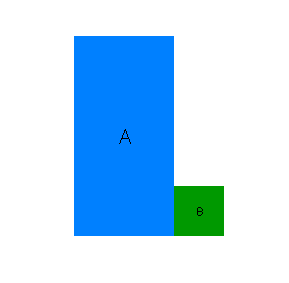
\includegraphics[width=0.2\textwidth]{cp1819t_media/ex2.png}
%
\caption{Caixa simples e caixa composta.\label{fig:L2D}}
\end{figure}

\begin{figure}
\centering
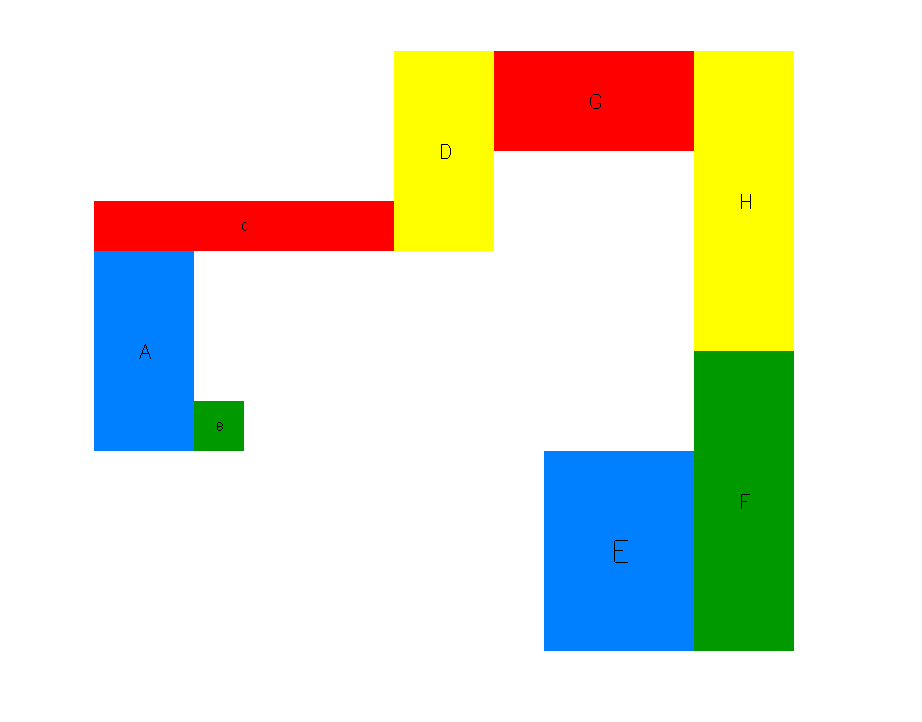
\includegraphics[width=0.6\textwidth]{cp1819t_media/ex.png}
\caption{\uk{Layout} feito de várias caixas coloridas.\label{fig:L2D1}}
\end{figure}

É importante notar que cada ``caixa'' não dispõe informação relativa
ao seu posicionamento final na figura. De facto, é a posição relativa
que deve ocupar face às restantes caixas que irá determinar a sua
posição final. Este é um dos objectivos deste trabalho:
\emph{calcular o posicionamento absoluto de cada uma das caixas por forma a
respeitar as restrições impostas pelas diversas agregações}. Para isso vamos
considerar um tipo de dados que comporta a informação de todas as
caixas devidamente posicionadas (i.e. com a informação adicional da
origem onde a caixa deve ser colocada).

\begin{hscode}\SaveRestoreHook
\column{B}{@{}>{\hspre}l<{\hspost}@{}}%
\column{E}{@{}>{\hspre}l<{\hspost}@{}}%
\>[B]{}\mathbf{type}\;\Conid{Fig}\mathrel{=}[\mskip1.5mu (\Conid{Origem},\Conid{Caixa})\mskip1.5mu]{}\<[E]%
\\
\>[B]{}\mathbf{type}\;\Conid{Origem}\mathrel{=}(\Conid{Float},\Conid{Float}){}\<[E]%
\ColumnHook
\end{hscode}\resethooks
%
A informação mais relevante deste tipo é a referente à lista de
``caixas posicionadas'' (tipo \ensuremath{(\Conid{Origem},\Conid{Caixa})}). Regista-se aí a origem
da caixa que, com a informação da sua altura e comprimento, permite
definir todos os seus pontos (consideramos as caixas sempre paralelas
aos eixos).

\begin{enumerate}
\item Forneça a definição da função \ensuremath{\Varid{calc\char95 origems}}, que calcula as
coordenadas iniciais das caixas no plano:
\begin{hscode}\SaveRestoreHook
\column{B}{@{}>{\hspre}l<{\hspost}@{}}%
\column{E}{@{}>{\hspre}l<{\hspost}@{}}%
\>[B]{}\Varid{calc\char95 origems}\mathbin{::}(\Conid{L2D},\Conid{Origem})\to \Conid{X}\;(\Conid{Caixa},\Conid{Origem})\;(){}\<[E]%
\ColumnHook
\end{hscode}\resethooks
\item Forneça agora a definição da função \ensuremath{\Varid{agrup\char95 caixas}}, que agrupa
todas as caixas e respectivas origens numa só lista:
\begin{hscode}\SaveRestoreHook
\column{B}{@{}>{\hspre}l<{\hspost}@{}}%
\column{E}{@{}>{\hspre}l<{\hspost}@{}}%
\>[B]{}\Varid{agrup\char95 caixas}\mathbin{::}\Conid{X}\;(\Conid{Caixa},\Conid{Origem})\;()\to \Conid{Fig}{}\<[E]%
\ColumnHook
\end{hscode}\resethooks
\end{enumerate}

Um segundo problema neste projecto é \emph{descobrir como visualizar a
informação gráfica calculada por \ensuremath{\Varid{desenho}}}. A nossa estratégia para
superar o problema baseia-se na biblioteca \gloss{Gloss}, que permite a geração
de gráficos 2D. Para tal disponibiliza-se a função
\begin{hscode}\SaveRestoreHook
\column{B}{@{}>{\hspre}l<{\hspost}@{}}%
\column{20}{@{}>{\hspre}l<{\hspost}@{}}%
\column{E}{@{}>{\hspre}l<{\hspost}@{}}%
\>[B]{}\Varid{crCaixa}\mathbin{::}\Conid{Origem}{}\<[20]%
\>[20]{}\to \Conid{Float}\to \Conid{Float}\to \Conid{String}\to \Conid{\Conid{G}.Color}\to \Conid{\Conid{G}.Picture}{}\<[E]%
\ColumnHook
\end{hscode}\resethooks
que cria um rectângulo com base numa coordenada, um valor para a largura, um valor
para a altura, um texto que irá servir de etiqueta, e a cor pretendida.
Disponibiliza-se também a função
\begin{hscode}\SaveRestoreHook
\column{B}{@{}>{\hspre}l<{\hspost}@{}}%
\column{E}{@{}>{\hspre}l<{\hspost}@{}}%
\>[B]{}\Varid{display}\mathbin{::}\Conid{\Conid{G}.Picture}\to \fun{IO}\;(){}\<[E]%
\ColumnHook
\end{hscode}\resethooks
que dado um valor do tipo \ensuremath{\Varid{\Conid{G}.picture}} abre uma janela com esse valor desenhado. O objectivo
final deste exercício é implementar então uma função
\begin{hscode}\SaveRestoreHook
\column{B}{@{}>{\hspre}l<{\hspost}@{}}%
\column{E}{@{}>{\hspre}l<{\hspost}@{}}%
\>[B]{}\Varid{mostra\char95 caixas}\mathbin{::}(\Conid{L2D},\Conid{Origem})\to \fun{IO}\;(){}\<[E]%
\ColumnHook
\end{hscode}\resethooks
que dada uma frase da linguagem \ensuremath{\Conid{L2D}} e coordenadas iniciais apresenta
o respectivo desenho no ecrã.
%
\textbf{Sugestão}:
Use a função \ensuremath{\Varid{\Conid{G}.pictures}} disponibilizada na biblioteca \gloss{Gloss}.

\Problema

Nesta disciplina estudou-se como fazer \pd{programação dinâmica} por cálculo,
recorrendo à lei de recursividade mútua.\footnote{Lei (\ref{eq:fokkinga})
em \cite{Ol18}, página \pageref{eq:fokkinga}.}

Para o caso de funções sobre os números naturais (\ensuremath{\N_0}, com functor \ensuremath{\fun F \;\Conid{X}\mathrel{=}\mathrm{1}\mathbin{+}\Conid{X}}) é fácil derivar-se da lei que foi estudada uma
	\emph{regra de algibeira}
	\label{pg:regra}
que se pode ensinar a programadores que não tenham estudado
\cp{Cálculo de Programas}. Apresenta-se de seguida essa regra, tomando como exemplo o
cálculo do ciclo-\textsf{for} que implementa a função de Fibonacci, recordar
o sistema
\begin{hscode}\SaveRestoreHook
\column{B}{@{}>{\hspre}l<{\hspost}@{}}%
\column{E}{@{}>{\hspre}l<{\hspost}@{}}%
\>[B]{}\Varid{fib}\;\mathrm{0}\mathrel{=}\mathrm{1}{}\<[E]%
\\
\>[B]{}\Varid{fib}\;(\Varid{n}\mathbin{+}\mathrm{1})\mathrel{=}\Varid{f}\;\Varid{n}{}\<[E]%
\\[\blanklineskip]%
\>[B]{}\Varid{f}\;\mathrm{0}\mathrel{=}\mathrm{1}{}\<[E]%
\\
\>[B]{}\Varid{f}\;(\Varid{n}\mathbin{+}\mathrm{1})\mathrel{=}\Varid{fib}\;\Varid{n}\mathbin{+}\Varid{f}\;\Varid{n}{}\<[E]%
\ColumnHook
\end{hscode}\resethooks
Obter-se-á de imediato
\begin{hscode}\SaveRestoreHook
\column{B}{@{}>{\hspre}l<{\hspost}@{}}%
\column{4}{@{}>{\hspre}l<{\hspost}@{}}%
\column{E}{@{}>{\hspre}l<{\hspost}@{}}%
\>[B]{}\Varid{fib'}\mathrel{=}\p1\comp \for{\Varid{loop}}\ {\Varid{init}}\;\mathbf{where}{}\<[E]%
\\
\>[B]{}\hsindent{4}{}\<[4]%
\>[4]{}\Varid{loop}\;(\Varid{fib},\Varid{f})\mathrel{=}(\Varid{f},\Varid{fib}\mathbin{+}\Varid{f}){}\<[E]%
\\
\>[B]{}\hsindent{4}{}\<[4]%
\>[4]{}\Varid{init}\mathrel{=}(\mathrm{1},\mathrm{1}){}\<[E]%
\ColumnHook
\end{hscode}\resethooks
usando as regras seguintes:
\begin{itemize}
\item	O corpo do ciclo \ensuremath{\Varid{loop}} terá tantos argumentos quanto o número de funções mutuamente recursivas.
\item	Para as variáveis escolhem-se os próprios nomes das funções, pela ordem
que se achar conveniente.\footnote{Podem obviamente usar-se outros símbolos, mas numa primeiraleitura
dá jeito usarem-se tais nomes.}
\item	Para os resultados vão-se buscar as expressões respectivas, retirando a variável \ensuremath{\Varid{n}}.
\item	Em \ensuremath{\Varid{init}} coleccionam-se os resultados dos casos de base das funções, pela mesma ordem.
\end{itemize}
Mais um exemplo, envolvendo polinómios no segundo grau a $x^2 + b x + c$ em \ensuremath{\N_0}.
Seguindo o método estudado nas aulas\footnote{Secção 3.17 de \cite{Ol18}.},
de $f\ x = a x^2 + b x + c$ derivam-se duas funções mutuamente recursivas:
\begin{hscode}\SaveRestoreHook
\column{B}{@{}>{\hspre}l<{\hspost}@{}}%
\column{E}{@{}>{\hspre}l<{\hspost}@{}}%
\>[B]{}\Varid{f}\;\mathrm{0}\mathrel{=}\Varid{c}{}\<[E]%
\\
\>[B]{}\Varid{f}\;(\Varid{n}\mathbin{+}\mathrm{1})\mathrel{=}\Varid{f}\;\Varid{n}\mathbin{+}\Varid{k}\;\Varid{n}{}\<[E]%
\\[\blanklineskip]%
\>[B]{}\Varid{k}\;\mathrm{0}\mathrel{=}\Varid{a}\mathbin{+}\Varid{b}{}\<[E]%
\\
\>[B]{}\Varid{k}\;(\Varid{n}\mathbin{+}\mathrm{1})\mathrel{=}\Varid{k}\;\Varid{n}\mathbin{+}\mathrm{2}\;\Varid{a}{}\<[E]%
\ColumnHook
\end{hscode}\resethooks
Seguindo a regra acima, calcula-se de imediato a seguinte implementação, em Haskell:
\begin{hscode}\SaveRestoreHook
\column{B}{@{}>{\hspre}l<{\hspost}@{}}%
\column{3}{@{}>{\hspre}l<{\hspost}@{}}%
\column{E}{@{}>{\hspre}l<{\hspost}@{}}%
\>[B]{}\Varid{f'}\;\Varid{a}\;\Varid{b}\;\Varid{c}\mathrel{=}\p1\comp \for{\Varid{loop}}\ {\Varid{init}}\;\mathbf{where}{}\<[E]%
\\
\>[B]{}\hsindent{3}{}\<[3]%
\>[3]{}\Varid{loop}\;(\Varid{f},\Varid{k})\mathrel{=}(\Varid{f}\mathbin{+}\Varid{k},\Varid{k}\mathbin{+}\mathrm{2}\mathbin{*}\Varid{a}){}\<[E]%
\\
\>[B]{}\hsindent{3}{}\<[3]%
\>[3]{}\Varid{init}\mathrel{=}(\Varid{c},\Varid{a}\mathbin{+}\Varid{b}){}\<[E]%
\ColumnHook
\end{hscode}\resethooks

Qual é o assunto desta questão, então? Considerem fórmula que dá a série de Taylor da
função coseno:
\begin{eqnarray*}
	cos\ x = \sum_{i=0}^\infty \frac{(-1)^i}{(2i)!} x^{2i}
\end{eqnarray*}
Pretende-se o ciclo-\textsf{for} que implementa a função
\ensuremath{\Varid{cos'}\;\Varid{x}\;\Varid{n}} que dá o valor dessa série tomando \ensuremath{\Varid{i}} até \ensuremath{\Varid{n}} inclusivé:
\begin{hscode}\SaveRestoreHook
\column{B}{@{}>{\hspre}l<{\hspost}@{}}%
\column{E}{@{}>{\hspre}l<{\hspost}@{}}%
\>[B]{}\Varid{cos'}\;\Varid{x}\mathrel{=}\cdots \comp \for{\Varid{loop}}\ {\Varid{init}}\;\mathbf{where}\;\cdots {}\<[E]%
\ColumnHook
\end{hscode}\resethooks
%
\textbf{Sugestão}: Começar por estudar muito bem o processo de cálculo dado
no anexo \ref{sec:recmul} para o problema (semelhante) da função exponencial.

\begin{propriedade}
Testes de que \ensuremath{\Varid{cos'}\;\Varid{x}} calcula bem o coseno de \ensuremath{\pi } e o coseno de \ensuremath{\pi \mathbin{/}\mathrm{2}}:
\begin{hscode}\SaveRestoreHook
\column{B}{@{}>{\hspre}l<{\hspost}@{}}%
\column{E}{@{}>{\hspre}l<{\hspost}@{}}%
\>[B]{}\Varid{prop\char95 cos1}\;\Varid{n}\mathrel{=}\Varid{n}\geq \mathrm{10}\Rightarrow\Varid{abs}\;(\Varid{cos}\;\pi \mathbin{-}\Varid{cos'}\;\pi \;\Varid{n})\mathbin{<}\mathrm{0.001}{}\<[E]%
\\
\>[B]{}\Varid{prop\char95 cos2}\;\Varid{n}\mathrel{=}\Varid{n}\geq \mathrm{10}\Rightarrow\Varid{abs}\;(\Varid{cos}\;(\pi \mathbin{/}\mathrm{2})\mathbin{-}\Varid{cos'}\;(\pi \mathbin{/}\mathrm{2})\;\Varid{n})\mathbin{<}\mathrm{0.001}{}\<[E]%
\ColumnHook
\end{hscode}\resethooks
\end{propriedade}

\paragraph{Valorização} Transliterar \ensuremath{\Varid{cos'}} para a linguagem C; compilar
e testar o código. Conseguia, por intuição apenas, chegar a esta função?

\Problema

Pretende-se nesta questão desenvolver uma biblioteca de funções para
manipular \emph{sistemas de ficheiros} genéricos.
Um sistema de ficheiros será visto como uma associação de \emph{nomes}
a ficheiros ou \emph{directorias}.
Estas últimas serão vistas como sub-sistemas de ficheiros e assim
recursivamente.
Assumindo que \ensuremath{\Varid{a}} é o tipo dos identificadores dos ficheiros e
directorias, e que \ensuremath{\Varid{b}} é o tipo do conteúdo dos ficheiros,
podemos definir um tipo indutivo de dados para representar sistemas de
ficheiros da seguinte forma:
\begin{hscode}\SaveRestoreHook
\column{B}{@{}>{\hspre}l<{\hspost}@{}}%
\column{E}{@{}>{\hspre}l<{\hspost}@{}}%
\>[B]{}\mathbf{data}\;\Conid{FS}\;\Varid{a}\;\Varid{b}\mathrel{=}\Conid{FS}\;[\mskip1.5mu (\Varid{a},\Conid{Node}\;\Varid{a}\;\Varid{b})\mskip1.5mu]\;\mathbf{deriving}\;(\Conid{Eq},\Conid{Show}){}\<[E]%
\\
\>[B]{}\mathbf{data}\;\Conid{Node}\;\Varid{a}\;\Varid{b}\mathrel{=}\Conid{File}\;\Varid{b}\mid \Conid{Dir}\;(\Conid{FS}\;\Varid{a}\;\Varid{b})\;\mathbf{deriving}\;(\Conid{Eq},\Conid{Show}){}\<[E]%
\ColumnHook
\end{hscode}\resethooks
Um caminho (\emph{path}) neste sistema de ficheiros pode ser representado pelo
seguinte tipo de dados:
\begin{hscode}\SaveRestoreHook
\column{B}{@{}>{\hspre}l<{\hspost}@{}}%
\column{E}{@{}>{\hspre}l<{\hspost}@{}}%
\>[B]{}\mathbf{type}\;\Conid{Path}\;\Varid{a}\mathrel{=}[\mskip1.5mu \Varid{a}\mskip1.5mu]{}\<[E]%
\ColumnHook
\end{hscode}\resethooks
Assumindo estes tipos de dados, o seguinte termo
\begin{hscode}\SaveRestoreHook
\column{B}{@{}>{\hspre}l<{\hspost}@{}}%
\column{4}{@{}>{\hspre}c<{\hspost}@{}}%
\column{4E}{@{}l@{}}%
\column{5}{@{}>{\hspre}l<{\hspost}@{}}%
\column{20}{@{}>{\hspre}l<{\hspost}@{}}%
\column{21}{@{}>{\hspre}l<{\hspost}@{}}%
\column{E}{@{}>{\hspre}l<{\hspost}@{}}%
\>[B]{}\Conid{FS}\;[\mskip1.5mu (\text{\ttfamily \char34 f1\char34},\Conid{File}\;\text{\ttfamily \char34 Ola\char34}),{}\<[E]%
\\
\>[B]{}\hsindent{5}{}\<[5]%
\>[5]{}(\text{\ttfamily \char34 d1\char34},\Conid{Dir}\;(\Conid{FS}\;[\mskip1.5mu (\text{\ttfamily \char34 f2\char34},\Conid{File}\;\text{\ttfamily \char34 Ole\char34}),{}\<[E]%
\\
\>[5]{}\hsindent{16}{}\<[21]%
\>[21]{}(\text{\ttfamily \char34 f3\char34},\Conid{File}\;\text{\ttfamily \char34 Ole\char34}){}\<[E]%
\\
\>[5]{}\hsindent{15}{}\<[20]%
\>[20]{}\mskip1.5mu])){}\<[E]%
\\
\>[B]{}\hsindent{4}{}\<[4]%
\>[4]{}\mskip1.5mu]{}\<[4E]%
\ColumnHook
\end{hscode}\resethooks
representará um sistema de ficheiros em cuja raíz temos um ficheiro chamado
\ensuremath{\Varid{f1}} com conteúdo \ensuremath{\text{\ttfamily \char34 Ola\char34}} e uma directoria chamada \ensuremath{\text{\ttfamily \char34 d1\char34}} constituída por dois
ficheiros, um chamado \ensuremath{\text{\ttfamily \char34 f2\char34}} e outro chamado \ensuremath{\text{\ttfamily \char34 f3\char34}}, ambos com conteúdo \ensuremath{\text{\ttfamily \char34 Ole\char34}}.
%
Neste caso, tanto o tipo dos identificadores como o tipo do conteúdo dos
ficheiros é \ensuremath{\Conid{String}}. No caso geral, o conteúdo de um ficheiro é arbitrário:
pode ser um binário, um texto, uma colecção de dados, etc.

A definição das usuais funções \ensuremath{\Varid{inFS}} e \ensuremath{\Varid{recFS}} para este tipo é a seguinte:
\begin{hscode}\SaveRestoreHook
\column{B}{@{}>{\hspre}l<{\hspost}@{}}%
\column{E}{@{}>{\hspre}l<{\hspost}@{}}%
\>[B]{}\Varid{inFS}\mathrel{=}\Conid{FS}\comp \map \;(\Varid{id}\times\Varid{inNode}){}\<[E]%
\\
\>[B]{}\Varid{inNode}\mathrel{=}\alt{\Conid{File}}{\Conid{Dir}}{}\<[E]%
\\[\blanklineskip]%
\>[B]{}\Varid{recFS}\;\Varid{f}\mathrel{=}\Varid{baseFS}\;\Varid{id}\;\Varid{id}\;\Varid{f}{}\<[E]%
\ColumnHook
\end{hscode}\resethooks
Suponha que se pretende definir como um \ensuremath{\Varid{catamorfismo}} a função que
conta o número de ficheiros existentes num sistema de ficheiros. Uma
possível definição para esta função seria:
\begin{hscode}\SaveRestoreHook
\column{B}{@{}>{\hspre}l<{\hspost}@{}}%
\column{E}{@{}>{\hspre}l<{\hspost}@{}}%
\>[B]{}\Varid{conta}\mathbin{::}\Conid{FS}\;\Varid{a}\;\Varid{b}\to \Conid{Int}{}\<[E]%
\\
\>[B]{}\Varid{conta}\mathrel{=}\Varid{cataFS}\;(\Varid{sum}\comp \map \;(\alt{\underline{\mathrm{1}}}{\Varid{id}}\comp \p2)){}\<[E]%
\ColumnHook
\end{hscode}\resethooks
O que é para fazer:
\begin{enumerate}
\item Definir as funções \ensuremath{\Varid{outFS}}, \ensuremath{\Varid{baseFS}}, \ensuremath{\Varid{cataFS}}, \ensuremath{\Varid{anaFS}} e \ensuremath{\Varid{hyloFS}}.

\item Apresentar, no relatório, o diagrama de \ensuremath{\Varid{cataFS}}.

\item Definir as seguintes funções para manipulação de sistemas de
  ficheiros usando, obrigatoriamente, catamorfismos, anamorfismos ou
  hilomorfismos:

  \begin{enumerate}
  \item Verificação da integridade do sistema de ficheiros (i.e. verificar
    que não existem identificadores repetidos dentro da mesma directoria). \\
    \ensuremath{\Varid{check}\mathbin{::}\Conid{FS}\;\Varid{a}\;\Varid{b}\to \Conid{Bool}}
  \begin{propriedade}
    A integridade de um sistema de ficheiros não depende da ordem em que os
    últimos são listados na sua directoria:
\begin{hscode}\SaveRestoreHook
\column{B}{@{}>{\hspre}l<{\hspost}@{}}%
\column{E}{@{}>{\hspre}l<{\hspost}@{}}%
\>[B]{}\Varid{prop\char95 check}\mathbin{::}\Conid{FS}\;\Conid{String}\;\Conid{String}\to \Conid{Bool}{}\<[E]%
\\
\>[B]{}\Varid{prop\char95 check}\mathrel{=}\Varid{check}\comp (\Varid{cataFS}\;(\Varid{inFS}\comp \Varid{reverse}))\equiv\Varid{check}{}\<[E]%
\ColumnHook
\end{hscode}\resethooks
  \end{propriedade}
  \item Recolha do conteúdo de todos os ficheiros num arquivo indexado pelo \emph{path}.\\
    \ensuremath{\Varid{tar}\mathbin{::}\Conid{FS}\;\Varid{a}\;\Varid{b}\to [\mskip1.5mu (\Conid{Path}\;\Varid{a},\Varid{b})\mskip1.5mu]}
  \begin{propriedade}
    O número de ficheiros no sistema deve ser igual ao número de ficheiros
    listados pela função \ensuremath{\Varid{tar}}.
\begin{hscode}\SaveRestoreHook
\column{B}{@{}>{\hspre}l<{\hspost}@{}}%
\column{E}{@{}>{\hspre}l<{\hspost}@{}}%
\>[B]{}\Varid{prop\char95 tar}\mathbin{::}\Conid{FS}\;\Conid{String}\;\Conid{String}\to \Conid{Bool}{}\<[E]%
\\
\>[B]{}\Varid{prop\char95 tar}\mathrel{=}\length \comp \Varid{tar}\equiv\Varid{conta}{}\<[E]%
\ColumnHook
\end{hscode}\resethooks
  \end{propriedade}
  \item Transformação de um arquivo com o conteúdo dos ficheiros
    indexado pelo \emph{path} num sistema de ficheiros.\\
    \ensuremath{\Varid{untar}\mathbin{::}[\mskip1.5mu (\Conid{Path}\;\Varid{a},\Varid{b})\mskip1.5mu]\to \Conid{FS}\;\Varid{a}\;\Varid{b}} \\
  \textbf{Sugestão}: Use a função \ensuremath{\Varid{joinDupDirs}} para juntar directorias que estejam na mesma
  pasta e que possuam o mesmo identificador.
  \begin{propriedade}
    A composição \ensuremath{\Varid{tar}\comp \Varid{untar}} preserva o número de ficheiros no sistema.
\begin{hscode}\SaveRestoreHook
\column{B}{@{}>{\hspre}l<{\hspost}@{}}%
\column{E}{@{}>{\hspre}l<{\hspost}@{}}%
\>[B]{}\Varid{prop\char95 untar}\mathbin{::}[\mskip1.5mu (\Conid{Path}\;\Conid{String},\Conid{String})\mskip1.5mu]\to \Conid{Property}{}\<[E]%
\\
\>[B]{}\Varid{prop\char95 untar}\mathrel{=}\Varid{validPaths}\Rightarrow((\length \comp \Varid{tar}\comp \Varid{untar})\equiv\length ){}\<[E]%
\\
\>[B]{}\Varid{validPaths}\mathbin{::}[\mskip1.5mu (\Conid{Path}\;\Conid{String},\Conid{String})\mskip1.5mu]\to \Conid{Bool}{}\<[E]%
\\
\>[B]{}\Varid{validPaths}\mathrel{=}(\equiv \mathrm{0})\comp \length \comp (\Varid{filter}\;(\lambda (\Varid{a},\anonymous )\to \length \;\Varid{a}\equiv \mathrm{0})){}\<[E]%
\ColumnHook
\end{hscode}\resethooks
\end{propriedade}
  \item Localização de todos os \emph{paths} onde existe um
    determinado ficheiro.\\
    \ensuremath{\Varid{find}\mathbin{::}\Varid{a}\to \Conid{FS}\;\Varid{a}\;\Varid{b}\to [\mskip1.5mu \Conid{Path}\;\Varid{a}\mskip1.5mu]}
  \begin{propriedade}
    A composição \ensuremath{\Varid{tar}\comp \Varid{untar}} preserva todos os ficheiros no sistema.
\begin{hscode}\SaveRestoreHook
\column{B}{@{}>{\hspre}l<{\hspost}@{}}%
\column{7}{@{}>{\hspre}l<{\hspost}@{}}%
\column{E}{@{}>{\hspre}l<{\hspost}@{}}%
\>[B]{}\Varid{prop\char95 find}\mathbin{::}\Conid{String}\to \Conid{FS}\;\Conid{String}\;\Conid{String}\to \Conid{Bool}{}\<[E]%
\\
\>[B]{}\Varid{prop\char95 find}\mathrel{=}\Varid{curry}\mathbin{\$}{}\<[E]%
\\
\>[B]{}\hsindent{7}{}\<[7]%
\>[7]{}\length \comp \uncurry{\Varid{find}}\equiv\length \comp \uncurry{\Varid{find}}\comp (\Varid{id}\times(\Varid{untar}\comp \Varid{tar})){}\<[E]%
\ColumnHook
\end{hscode}\resethooks
  \end{propriedade}
  \item Criação de um novo ficheiro num determinado \emph{path}.\\
    \ensuremath{\Varid{new}\mathbin{::}\Conid{Path}\;\Varid{a}\to \Varid{b}\to \Conid{FS}\;\Varid{a}\;\Varid{b}\to \Conid{FS}\;\Varid{a}\;\Varid{b}}
  \begin{propriedade}
A adição de um ficheiro não existente no sistema não origina ficheiros duplicados.
\begin{hscode}\SaveRestoreHook
\column{B}{@{}>{\hspre}l<{\hspost}@{}}%
\column{7}{@{}>{\hspre}l<{\hspost}@{}}%
\column{47}{@{}>{\hspre}l<{\hspost}@{}}%
\column{E}{@{}>{\hspre}l<{\hspost}@{}}%
\>[B]{}\Varid{prop\char95 new}\mathbin{::}((\Conid{Path}\;\Conid{String},\Conid{String}),\Conid{FS}\;\Conid{String}\;\Conid{String})\to \Conid{Property}{}\<[E]%
\\
\>[B]{}\Varid{prop\char95 new}\mathrel{=}((\Varid{validPath}\wedge\Varid{notDup})\wedge(\Varid{check}\comp \p2))\Rightarrow{}\<[E]%
\\
\>[B]{}\hsindent{7}{}\<[7]%
\>[7]{}(\Varid{checkFiles}\comp \uncurry{\uncurry{\Varid{new}}})\;{}\<[47]%
\>[47]{}\mathbf{where}{}\<[E]%
\\
\>[B]{}\hsindent{7}{}\<[7]%
\>[7]{}\Varid{validPath}\mathrel{=}(\not\equiv \mathrm{0})\comp \length \comp \p1\comp \p1{}\<[E]%
\\
\>[B]{}\hsindent{7}{}\<[7]%
\>[7]{}\Varid{notDup}\mathrel{=}\neg \comp \uncurry{\Varid{elem}}\comp (\p1\times((\mathsf{fmap}\;\p1)\comp \Varid{tar})){}\<[E]%
\ColumnHook
\end{hscode}\resethooks
\textbf{Questão}: Supondo-se que no código acima se substitui a propriedade
\ensuremath{\Varid{checkFiles}} pela propriedade mais fraca \ensuremath{\Varid{check}}, será que a propriedade
\ensuremath{\Varid{prop\char95 new}} ainda é válida? Justifique a sua resposta.
\end{propriedade}

\begin{propriedade}
	A listagem de ficheiros logo após uma adição nunca poderá ser menor que a listagem
	de ficheiros antes dessa mesma adição.
\begin{hscode}\SaveRestoreHook
\column{B}{@{}>{\hspre}l<{\hspost}@{}}%
\column{7}{@{}>{\hspre}l<{\hspost}@{}}%
\column{E}{@{}>{\hspre}l<{\hspost}@{}}%
\>[B]{}\Varid{prop\char95 new2}\mathbin{::}((\Conid{Path}\;\Conid{String},\Conid{String}),\Conid{FS}\;\Conid{String}\;\Conid{String})\to \Conid{Property}{}\<[E]%
\\
\>[B]{}\Varid{prop\char95 new2}\mathrel{=}\Varid{validPath}\Rightarrow((\length \comp \Varid{tar}\comp \p2)\leq(\length \comp \Varid{tar}\comp \uncurry{\uncurry{\Varid{new}}}))\;\mathbf{where}{}\<[E]%
\\
\>[B]{}\hsindent{7}{}\<[7]%
\>[7]{}\Varid{validPath}\mathrel{=}(\not\equiv \mathrm{0})\comp \length \comp \p1\comp \p1{}\<[E]%
\ColumnHook
\end{hscode}\resethooks
  \end{propriedade}
  \item Duplicação de um ficheiro.\\
    \ensuremath{\Varid{cp}\mathbin{::}\Conid{Path}\;\Varid{a}\to \Conid{Path}\;\Varid{a}\to \Conid{FS}\;\Varid{a}\;\Varid{b}\to \Conid{FS}\;\Varid{a}\;\Varid{b}}
  \begin{propriedade}
    A listagem de ficheiros com um dado nome não diminui após uma duplicação.
\begin{hscode}\SaveRestoreHook
\column{B}{@{}>{\hspre}l<{\hspost}@{}}%
\column{13}{@{}>{\hspre}l<{\hspost}@{}}%
\column{42}{@{}>{\hspre}l<{\hspost}@{}}%
\column{E}{@{}>{\hspre}l<{\hspost}@{}}%
\>[B]{}\Varid{prop\char95 cp}\mathbin{::}((\Conid{Path}\;\Conid{String},\Conid{Path}\;\Conid{String}),{}\<[42]%
\>[42]{}\Conid{FS}\;\Conid{String}\;\Conid{String})\to \Conid{Bool}{}\<[E]%
\\
\>[B]{}\Varid{prop\char95 cp}\mathrel{=}{}\<[13]%
\>[13]{}\length \comp \Varid{tar}\comp \p2\leq\length \comp \Varid{tar}\comp \uncurry{\uncurry{\Varid{cp}}}{}\<[E]%
\ColumnHook
\end{hscode}\resethooks
  \end{propriedade}
  \item Eliminação de um ficheiro.\\
    \ensuremath{\Varid{rm}\mathbin{::}\Conid{Path}\;\Varid{a}\to \Conid{FS}\;\Varid{a}\;\Varid{b}\to \Conid{FS}\;\Varid{a}\;\Varid{b}}

  \textbf{Sugestão}: Construir um anamorfismo \ensuremath{\Varid{nav}\mathbin{::}(\Conid{Path}\;\Varid{a},\Conid{FS}\;\Varid{a}\;\Varid{b})\to \Conid{FS}\;\Varid{a}\;\Varid{b}}
  que navegue por um sistema de ficheiros tendo como base o \ensuremath{\Varid{path}} dado como argumento.
    \begin{propriedade}
    Remover duas vezes o mesmo ficheiro tem o mesmo efeito que o remover apenas uma vez.
\begin{hscode}\SaveRestoreHook
\column{B}{@{}>{\hspre}l<{\hspost}@{}}%
\column{E}{@{}>{\hspre}l<{\hspost}@{}}%
\>[B]{}\Varid{prop\char95 rm}\mathbin{::}(\Conid{Path}\;\Conid{String},\Conid{FS}\;\Conid{String}\;\Conid{String})\to \Conid{Bool}{}\<[E]%
\\
\>[B]{}\Varid{prop\char95 rm}\mathrel{=}\uncurry{\Varid{rm}}\comp \conj{\p1}{\uncurry{\Varid{rm}}}\equiv\uncurry{\Varid{rm}}{}\<[E]%
\ColumnHook
\end{hscode}\resethooks
\end{propriedade}
\begin{propriedade}
Adicionar um ficheiro e de seguida remover o mesmo não origina novos ficheiros no sistema.
\begin{hscode}\SaveRestoreHook
\column{B}{@{}>{\hspre}l<{\hspost}@{}}%
\column{10}{@{}>{\hspre}l<{\hspost}@{}}%
\column{23}{@{}>{\hspre}l<{\hspost}@{}}%
\column{E}{@{}>{\hspre}l<{\hspost}@{}}%
\>[B]{}\Varid{prop\char95 rm2}\mathbin{::}((\Conid{Path}\;\Conid{String},\Conid{String}),\Conid{FS}\;\Conid{String}\;\Conid{String})\to \Conid{Property}{}\<[E]%
\\
\>[B]{}\Varid{prop\char95 rm2}\mathrel{=}\Varid{validPath}{}\<[23]%
\>[23]{}\Rightarrow((\length \comp \Varid{tar}\comp \uncurry{\Varid{rm}}\comp \conj{\p1\comp \p1}{\uncurry{\uncurry{\Varid{new}}}}){}\<[E]%
\\
\>[B]{}\hsindent{10}{}\<[10]%
\>[10]{}\leq(\length \comp \Varid{tar}\comp \p2))\;\mathbf{where}{}\<[E]%
\\
\>[B]{}\hsindent{10}{}\<[10]%
\>[10]{}\Varid{validPath}\mathrel{=}(\not\equiv \mathrm{0})\comp \length \comp \p1\comp \p1{}\<[E]%
\ColumnHook
\end{hscode}\resethooks
\end{propriedade}
  \end{enumerate}
\end{enumerate}

\paragraph{Valorização}

Definir uma função para visualizar em \graphviz{Graphviz}
a estrutura de um sistema de ficheiros. A Figura~\ref{ex_prob1}, por exemplo,
apresenta a estrutura de um sistema com precisamente dois ficheiros dentro
de uma directoria chamada \ensuremath{\text{\ttfamily \char34 d1\char34}}.

Para realizar este exercício será necessário apenas  escrever o anamorfismo
\begin{quote}
\ensuremath{\Varid{cFS2Exp}\mathbin{::}(\Varid{a},\Conid{FS}\;\Varid{a}\;\Varid{b})\to (\Conid{Exp}\;()\;\Varid{a})}
\end{quote}
que converte a estrutura de um sistema de ficheiros numa árvore de expressões
descrita em \href{http://wiki.di.uminho.pt/twiki/pub/Education/CP/MaterialPedagogico/Exp.hs}{Exp.hs}.
A função \ensuremath{\Varid{dotFS}} depois tratará de passar a estrutura do sistema de ficheiros para o visualizador.
\begin{figure}
\centering
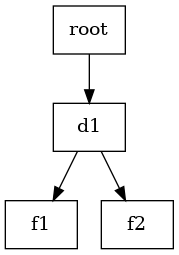
\includegraphics[scale=0.5]{cp1819t_media/fs.png}
\caption{Exemplo de um sistema de ficheiros visualizado em \graphviz{Graphviz}.}
\label{ex_prob1}
\end{figure}

%----------------- Programa, bibliotecas e código auxiliar --------------------%

\newpage

\part*{Anexos}

\appendix

\section{Como exprimir cálculos e diagramas em LaTeX/lhs2tex}
Estudar o texto fonte deste trabalho para obter o efeito:\footnote{Exemplos tirados de \cite{Ol18}.}
\begin{eqnarray*}
\start
	\ensuremath{\Varid{id}\mathrel{=}\conj{\Varid{f}}{\Varid{g}}}
%
\just\equiv{ universal property }
%
        \ensuremath{\begin{lcbr}\p1\comp \Varid{id}\mathrel{=}\Varid{f}\\\p2\comp \Varid{id}\mathrel{=}\Varid{g}\end{lcbr}}
%
\just\equiv{ identity }
%
        \ensuremath{\begin{lcbr}\p1\mathrel{=}\Varid{f}\\\p2\mathrel{=}\Varid{g}\end{lcbr}}
\qed
\end{eqnarray*}

Os diagramas podem ser produzidos recorrendo à \emph{package} \LaTeX\
\href{https://ctan.org/pkg/xymatrix}{xymatrix}, por exemplo:
\begin{eqnarray*}
\xymatrix@C=2cm{
    \ensuremath{\N_0}
           \ar[d]_-{\ensuremath{\cata{\Varid{g}}}}
&
    \ensuremath{\mathrm{1}\mathbin{+}\N_0}
           \ar[d]^{\ensuremath{\Varid{id}\mathbin{+}\cata{\Varid{g}}}}
           \ar[l]_-{\ensuremath{\mathsf{in}}}
\\
     \ensuremath{\Conid{B}}
&
     \ensuremath{\mathrm{1}\mathbin{+}\Conid{B}}
           \ar[l]^-{\ensuremath{\Varid{g}}}
}
\end{eqnarray*}

\section{Programação dinâmica por recursividade múltipla}\label{sec:recmul}
Neste anexo dão-se os detalhes da resolução do Exercício \ref{ex:exp} dos apontamentos da
disciplina\footnote{Cf.\ \cite{Ol18}, página \pageref{ex:exp}.},
onde se pretende implementar um ciclo que implemente
o cálculo da aproximação até \ensuremath{\Varid{i}\mathrel{=}\Varid{n}} da função exponencial $exp\ x = e^x$
via série de Taylor:
\begin{eqnarray}
	exp\ x
& = &
	\sum_{i=0}^{\infty} \frac {x^i} {i!}
\end{eqnarray}
Seja $e\ x\ n = \sum_{i=0}^{n} \frac {x^i} {i!}$ a função que dá essa aproximação.
É fácil de ver que \ensuremath{\Varid{e}\;\Varid{x}\;\mathrm{0}\mathrel{=}\mathrm{1}} e que $\ensuremath{\Varid{e}\;\Varid{x}\;(\Varid{n}\mathbin{+}\mathrm{1})} = \ensuremath{\Varid{e}\;\Varid{x}\;\Varid{n}} + \frac {x^{n+1}} {(n+1)!}$.
Se definirmos $\ensuremath{\Varid{h}\;\Varid{x}\;\Varid{n}} = \frac {x^{n+1}} {(n+1)!}$ teremos \ensuremath{\Varid{e}\;\Varid{x}} e \ensuremath{\Varid{h}\;\Varid{x}} em recursividade
mútua. Se repetirmos o processo para \ensuremath{\Varid{h}\;\Varid{x}\;\Varid{n}} etc obteremos no total três funções nessa mesma
situação:
\begin{hscode}\SaveRestoreHook
\column{B}{@{}>{\hspre}l<{\hspost}@{}}%
\column{E}{@{}>{\hspre}l<{\hspost}@{}}%
\>[B]{}\Varid{e}\;\Varid{x}\;\mathrm{0}\mathrel{=}\mathrm{1}{}\<[E]%
\\
\>[B]{}\Varid{e}\;\Varid{x}\;(\Varid{n}\mathbin{+}\mathrm{1})\mathrel{=}\Varid{h}\;\Varid{x}\;\Varid{n}\mathbin{+}\Varid{e}\;\Varid{x}\;\Varid{n}{}\<[E]%
\\[\blanklineskip]%
\>[B]{}\Varid{h}\;\Varid{x}\;\mathrm{0}\mathrel{=}\Varid{x}{}\<[E]%
\\
\>[B]{}\Varid{h}\;\Varid{x}\;(\Varid{n}\mathbin{+}\mathrm{1})\mathrel{=}\Varid{x}\mathbin{/}(\Varid{s}\;\Varid{n})\mathbin{*}\Varid{h}\;\Varid{x}\;\Varid{n}{}\<[E]%
\\[\blanklineskip]%
\>[B]{}\Varid{s}\;\mathrm{0}\mathrel{=}\mathrm{2}{}\<[E]%
\\
\>[B]{}\Varid{s}\;(\Varid{n}\mathbin{+}\mathrm{1})\mathrel{=}\mathrm{1}\mathbin{+}\Varid{s}\;\Varid{n}{}\<[E]%
\ColumnHook
\end{hscode}\resethooks
Segundo a \emph{regra de algibeira} descrita na página \ref{pg:regra} deste enunciado,
ter-se-á, de imediato:
\begin{hscode}\SaveRestoreHook
\column{B}{@{}>{\hspre}l<{\hspost}@{}}%
\column{6}{@{}>{\hspre}l<{\hspost}@{}}%
\column{E}{@{}>{\hspre}l<{\hspost}@{}}%
\>[B]{}\Varid{e'}\;\Varid{x}\mathrel{=}\Varid{prj}\comp \for{\Varid{loop}}\ {\Varid{init}}\;\mathbf{where}{}\<[E]%
\\
\>[B]{}\hsindent{6}{}\<[6]%
\>[6]{}\Varid{init}\mathrel{=}(\mathrm{1},\Varid{x},\mathrm{2}){}\<[E]%
\\
\>[B]{}\hsindent{6}{}\<[6]%
\>[6]{}\Varid{loop}\;(\Varid{e},\Varid{h},\Varid{s})\mathrel{=}(\Varid{h}\mathbin{+}\Varid{e},\Varid{x}\mathbin{/}\Varid{s}\mathbin{*}\Varid{h},\mathrm{1}\mathbin{+}\Varid{s}){}\<[E]%
\\
\>[B]{}\hsindent{6}{}\<[6]%
\>[6]{}\Varid{prj}\;(\Varid{e},\Varid{h},\Varid{s})\mathrel{=}\Varid{e}{}\<[E]%
\ColumnHook
\end{hscode}\resethooks

\section{Código fornecido}\label{sec:codigo}

\subsection*{Problema 1}
Tipos:
\begin{hscode}\SaveRestoreHook
\column{B}{@{}>{\hspre}l<{\hspost}@{}}%
\column{16}{@{}>{\hspre}l<{\hspost}@{}}%
\column{36}{@{}>{\hspre}l<{\hspost}@{}}%
\column{46}{@{}>{\hspre}l<{\hspost}@{}}%
\column{E}{@{}>{\hspre}l<{\hspost}@{}}%
\>[B]{}\mathbf{data}\;\Conid{Expr}\mathrel{=}\Conid{Num}\;\Conid{Int}{}\<[E]%
\\
\>[B]{}\hsindent{16}{}\<[16]%
\>[16]{}\mid \Conid{Bop}\;\Conid{Expr}\;\Conid{Op}\;\Conid{Expr}\;{}\<[36]%
\>[36]{}\mathbf{deriving}\;{}\<[46]%
\>[46]{}(\Conid{Eq},\Conid{Show}){}\<[E]%
\\[\blanklineskip]%
\>[B]{}\mathbf{data}\;\Conid{Op}\mathrel{=}\Conid{Op}\;\Conid{String}\;\mathbf{deriving}\;(\Conid{Eq},\Conid{Show}){}\<[E]%
\\[\blanklineskip]%
\>[B]{}\mathbf{type}\;\Conid{Codigo}\mathrel{=}[\mskip1.5mu \Conid{String}\mskip1.5mu]{}\<[E]%
\ColumnHook
\end{hscode}\resethooks
Functor de base:
\begin{hscode}\SaveRestoreHook
\column{B}{@{}>{\hspre}l<{\hspost}@{}}%
\column{E}{@{}>{\hspre}l<{\hspost}@{}}%
\>[B]{}\Varid{baseExpr}\;\Varid{f}\;\Varid{g}\mathrel{=}\Varid{id}+(\Varid{f}\times(\Varid{g}\times\Varid{g})){}\<[E]%
\ColumnHook
\end{hscode}\resethooks
Instâncias:
\begin{hscode}\SaveRestoreHook
\column{B}{@{}>{\hspre}l<{\hspost}@{}}%
\column{4}{@{}>{\hspre}l<{\hspost}@{}}%
\column{E}{@{}>{\hspre}l<{\hspost}@{}}%
\>[B]{}\mathbf{instance}\;\Conid{Read}\;\Conid{Expr}\;\mathbf{where}{}\<[E]%
\\
\>[B]{}\hsindent{4}{}\<[4]%
\>[4]{}\Varid{readsPrec}\;\anonymous \mathrel{=}\Varid{readExp}{}\<[E]%
\ColumnHook
\end{hscode}\resethooks
Read para Exp's:
\begin{hscode}\SaveRestoreHook
\column{B}{@{}>{\hspre}l<{\hspost}@{}}%
\column{10}{@{}>{\hspre}l<{\hspost}@{}}%
\column{11}{@{}>{\hspre}l<{\hspost}@{}}%
\column{18}{@{}>{\hspre}l<{\hspost}@{}}%
\column{20}{@{}>{\hspre}l<{\hspost}@{}}%
\column{21}{@{}>{\hspre}l<{\hspost}@{}}%
\column{E}{@{}>{\hspre}l<{\hspost}@{}}%
\>[B]{}\Varid{readOp}\mathbin{::}\Conid{String}\to [\mskip1.5mu (\Conid{Op},\Conid{String})\mskip1.5mu]{}\<[E]%
\\
\>[B]{}\Varid{readOp}\;\Varid{input}\mathrel{=}\mathbf{do}{}\<[E]%
\\
\>[B]{}\hsindent{18}{}\<[18]%
\>[18]{}(\Varid{x},\Varid{y})\leftarrow \Varid{lex}\;\Varid{input}{}\<[E]%
\\
\>[B]{}\hsindent{18}{}\<[18]%
\>[18]{}\Varid{return}\;((\Conid{Op}\;\Varid{x}),\Varid{y}){}\<[E]%
\\[\blanklineskip]%
\>[B]{}\Varid{readNum}\mathbin{::}\Conid{ReadS}\;\Conid{Expr}{}\<[E]%
\\
\>[B]{}\Varid{readNum}{}\<[10]%
\>[10]{}\mathrel{=}(\map \;(\lambda (\Varid{x},\Varid{y})\to ((\Conid{Num}\;\Varid{x}),\Varid{y})))\comp \Varid{reads}{}\<[E]%
\\[\blanklineskip]%
\>[B]{}\Varid{readBinOp}\mathbin{::}\Conid{ReadS}\;\Conid{Expr}{}\<[E]%
\\
\>[B]{}\Varid{readBinOp}\mathrel{=}(\map \;(\lambda ((\Varid{x},(\Varid{y},\Varid{z})),\Varid{t})\to ((\Conid{Bop}\;\Varid{x}\;\Varid{y}\;\Varid{z}),\Varid{t})))\comp {}\<[E]%
\\
\>[B]{}\hsindent{20}{}\<[20]%
\>[20]{}((\Varid{readNum}\mathbin{`\Varid{ou}`}(\Varid{pcurvos}\;\Varid{readExp})){}\<[E]%
\\
\>[20]{}\hsindent{1}{}\<[21]%
\>[21]{}\mathbin{`\Varid{depois}`}(\Varid{readOp}\mathbin{`\Varid{depois}`}\Varid{readExp})){}\<[E]%
\\[\blanklineskip]%
\>[B]{}\Varid{readExp}\mathbin{::}\Conid{ReadS}\;\Conid{Expr}{}\<[E]%
\\
\>[B]{}\Varid{readExp}\mathrel{=}\Varid{readBinOp}\mathbin{`\Varid{ou}`}({}\<[E]%
\\
\>[B]{}\hsindent{11}{}\<[11]%
\>[11]{}\Varid{readNum}\mathbin{`\Varid{ou}`}({}\<[E]%
\\
\>[B]{}\hsindent{11}{}\<[11]%
\>[11]{}\Varid{pcurvos}\;\Varid{readExp})){}\<[E]%
\ColumnHook
\end{hscode}\resethooks
Combinadores:
\begin{hscode}\SaveRestoreHook
\column{B}{@{}>{\hspre}l<{\hspost}@{}}%
\column{3}{@{}>{\hspre}l<{\hspost}@{}}%
\column{5}{@{}>{\hspre}l<{\hspost}@{}}%
\column{7}{@{}>{\hspre}l<{\hspost}@{}}%
\column{10}{@{}>{\hspre}l<{\hspost}@{}}%
\column{16}{@{}>{\hspre}l<{\hspost}@{}}%
\column{22}{@{}>{\hspre}l<{\hspost}@{}}%
\column{25}{@{}>{\hspre}l<{\hspost}@{}}%
\column{36}{@{}>{\hspre}l<{\hspost}@{}}%
\column{42}{@{}>{\hspre}l<{\hspost}@{}}%
\column{53}{@{}>{\hspre}l<{\hspost}@{}}%
\column{E}{@{}>{\hspre}l<{\hspost}@{}}%
\>[B]{}\Varid{depois}\mathbin{::}(\Conid{ReadS}\;\Varid{a})\to (\Conid{ReadS}\;\Varid{b})\to \Conid{ReadS}\;(\Varid{a},\Varid{b}){}\<[E]%
\\
\>[B]{}\Varid{depois}\;\anonymous \;\anonymous \;[\mskip1.5mu \mskip1.5mu]\mathrel{=}[\mskip1.5mu \mskip1.5mu]{}\<[E]%
\\
\>[B]{}\Varid{depois}\;\Varid{r1}\;\Varid{r2}\;\Varid{input}\mathrel{=}[\mskip1.5mu ((\Varid{x},\Varid{y}),i_2)\mid (\Varid{x},i_1)\leftarrow \Varid{r1}\;\Varid{input},{}\<[E]%
\\
\>[B]{}\hsindent{36}{}\<[36]%
\>[36]{}(\Varid{y},i_2)\leftarrow \Varid{r2}\;i_1\mskip1.5mu]{}\<[E]%
\\[\blanklineskip]%
\>[B]{}\Varid{readSeq}\mathbin{::}(\Conid{ReadS}\;\Varid{a})\to \Conid{ReadS}\;[\mskip1.5mu \Varid{a}\mskip1.5mu]{}\<[E]%
\\
\>[B]{}\Varid{readSeq}\;\Varid{r}\;\Varid{input}{}\<[E]%
\\
\>[B]{}\hsindent{3}{}\<[3]%
\>[3]{}\mathrel{=}\mathbf{case}\;(\Varid{r}\;\Varid{input})\;\mathbf{of}{}\<[E]%
\\
\>[3]{}\hsindent{2}{}\<[5]%
\>[5]{}[\mskip1.5mu \mskip1.5mu]\to [\mskip1.5mu ([\mskip1.5mu \mskip1.5mu],\Varid{input})\mskip1.5mu]{}\<[E]%
\\
\>[3]{}\hsindent{2}{}\<[5]%
\>[5]{}\Varid{l}\to \Varid{concat}\;(\map \;\Varid{continua}\;\Varid{l}){}\<[E]%
\\
\>[5]{}\hsindent{5}{}\<[10]%
\>[10]{}\mathbf{where}\;\Varid{continua}\;(\Varid{a},\Varid{i})\mathrel{=}\map \;(\Varid{c}\;\Varid{a})\;(\Varid{readSeq}\;\Varid{r}\;\Varid{i}){}\<[E]%
\\
\>[10]{}\hsindent{6}{}\<[16]%
\>[16]{}\Varid{c}\;\Varid{x}\;(\Varid{xs},\Varid{i})\mathrel{=}((\Varid{x}\mathbin{:}\Varid{xs}),\Varid{i}){}\<[E]%
\\[\blanklineskip]%
\>[B]{}\Varid{ou}\mathbin{::}(\Conid{ReadS}\;\Varid{a})\to (\Conid{ReadS}\;\Varid{a})\to \Conid{ReadS}\;\Varid{a}{}\<[E]%
\\
\>[B]{}\Varid{ou}\;\Varid{r1}\;\Varid{r2}\;\Varid{input}\mathrel{=}(\Varid{r1}\;\Varid{input})\plus (\Varid{r2}\;\Varid{input}){}\<[E]%
\\[\blanklineskip]%
\>[B]{}\Varid{senao}\mathbin{::}(\Conid{ReadS}\;\Varid{a})\to (\Conid{ReadS}\;\Varid{a})\to \Conid{ReadS}\;\Varid{a}{}\<[E]%
\\
\>[B]{}\Varid{senao}\;\Varid{r1}\;\Varid{r2}\;\Varid{input}\mathrel{=}\mathbf{case}\;(\Varid{r1}\;\Varid{input})\;\mathbf{of}{}\<[E]%
\\
\>[B]{}\hsindent{22}{}\<[22]%
\>[22]{}[\mskip1.5mu \mskip1.5mu]\to \Varid{r2}\;\Varid{input}{}\<[E]%
\\
\>[B]{}\hsindent{22}{}\<[22]%
\>[22]{}\Varid{l}{}\<[25]%
\>[25]{}\to \Varid{l}{}\<[E]%
\\[\blanklineskip]%
\>[B]{}\Varid{readConst}\mathbin{::}\Conid{String}\to \Conid{ReadS}\;\Conid{String}{}\<[E]%
\\
\>[B]{}\Varid{readConst}\;\Varid{c}\mathrel{=}(\Varid{filter}\;((\equiv \Varid{c})\comp \p1))\comp \Varid{lex}{}\<[E]%
\\[\blanklineskip]%
\>[B]{}\Varid{pcurvos}\mathrel{=}\Varid{parentesis}\;\text{\ttfamily '('}\;\text{\ttfamily ')'}{}\<[E]%
\\
\>[B]{}\Varid{prectos}\mathrel{=}\Varid{parentesis}\;\text{\ttfamily '['}\;\text{\ttfamily ']'}{}\<[E]%
\\
\>[B]{}\Varid{chavetas}\mathrel{=}\Varid{parentesis}\;\text{\ttfamily '\char123 '}\;\text{\ttfamily '\char125 '}{}\<[E]%
\\[\blanklineskip]%
\>[B]{}\Varid{parentesis}\mathbin{::}\Conid{Char}\to \Conid{Char}\to (\Conid{ReadS}\;\Varid{a})\to \Conid{ReadS}\;\Varid{a}{}\<[E]%
\\
\>[B]{}\Varid{parentesis}\;\anonymous \;\anonymous \;\anonymous \;[\mskip1.5mu \mskip1.5mu]\mathrel{=}[\mskip1.5mu \mskip1.5mu]{}\<[E]%
\\
\>[B]{}\Varid{parentesis}\;\Varid{ap}\;\Varid{pa}\;\Varid{r}\;\Varid{input}{}\<[E]%
\\
\>[B]{}\hsindent{3}{}\<[3]%
\>[3]{}\mathrel{=}\mathbf{do}{}\<[E]%
\\
\>[3]{}\hsindent{4}{}\<[7]%
\>[7]{}((\anonymous ,(\Varid{x},\anonymous )),\Varid{c})\leftarrow ((\Varid{readConst}\;[\mskip1.5mu \Varid{ap}\mskip1.5mu])\mathbin{`\Varid{depois}`}({}\<[E]%
\\
\>[7]{}\hsindent{18}{}\<[25]%
\>[25]{}\Varid{r}{}\<[42]%
\>[42]{}\mathbin{`\Varid{depois}`}({}\<[E]%
\\
\>[7]{}\hsindent{18}{}\<[25]%
\>[25]{}\Varid{readConst}\;[\mskip1.5mu \Varid{pa}\mskip1.5mu])))\;{}\<[53]%
\>[53]{}\Varid{input}{}\<[E]%
\\
\>[3]{}\hsindent{4}{}\<[7]%
\>[7]{}\Varid{return}\;(\Varid{x},\Varid{c}){}\<[E]%
\ColumnHook
\end{hscode}\resethooks

\subsection*{Problema 2}
Tipos:
\begin{hscode}\SaveRestoreHook
\column{B}{@{}>{\hspre}l<{\hspost}@{}}%
\column{E}{@{}>{\hspre}l<{\hspost}@{}}%
\>[B]{}\mathbf{type}\;\Conid{Fig}\mathrel{=}[\mskip1.5mu (\Conid{Origem},\Conid{Caixa})\mskip1.5mu]{}\<[E]%
\\
\>[B]{}\mathbf{type}\;\Conid{Origem}\mathrel{=}(\Conid{Float},\Conid{Float}){}\<[E]%
\ColumnHook
\end{hscode}\resethooks
``Helpers":
\begin{hscode}\SaveRestoreHook
\column{B}{@{}>{\hspre}l<{\hspost}@{}}%
\column{E}{@{}>{\hspre}l<{\hspost}@{}}%
\>[B]{}\Varid{col\char95 blue}\mathrel{=}\Varid{\Conid{G}.azure}{}\<[E]%
\\
\>[B]{}\Varid{col\char95 green}\mathrel{=}\Varid{darkgreen}{}\<[E]%
\\[\blanklineskip]%
\>[B]{}\Varid{darkgreen}\mathrel{=}\Varid{\Conid{G}.dark}\;(\Varid{\Conid{G}.dark}\;\Varid{\Conid{G}.green}){}\<[E]%
\ColumnHook
\end{hscode}\resethooks
Exemplos:
\begin{hscode}\SaveRestoreHook
\column{B}{@{}>{\hspre}l<{\hspost}@{}}%
\column{11}{@{}>{\hspre}l<{\hspost}@{}}%
\column{14}{@{}>{\hspre}l<{\hspost}@{}}%
\column{E}{@{}>{\hspre}l<{\hspost}@{}}%
\>[B]{}\Varid{ex1Caixas}\mathrel{=}\Varid{\Conid{G}.display}\;(\Conid{\Conid{G}.InWindow}\;\text{\ttfamily \char34 Problema~4\char34}\;(\mathrm{400},\mathrm{400})\;(\mathrm{40},\mathrm{40}))\;\Varid{\Conid{G}.white}\mathbin{\$}{}\<[E]%
\\
\>[B]{}\hsindent{11}{}\<[11]%
\>[11]{}\Varid{crCaixa}\;(\mathrm{0},\mathrm{0})\;\mathrm{200}\;\mathrm{200}\;\text{\ttfamily \char34 Caixa~azul\char34}\;\Varid{col\char95 blue}{}\<[E]%
\\[\blanklineskip]%
\>[B]{}\Varid{ex2Caixas}\mathrel{=}{}\<[14]%
\>[14]{}\Varid{\Conid{G}.display}\;(\Conid{\Conid{G}.InWindow}\;\text{\ttfamily \char34 Problema~4\char34}\;(\mathrm{400},\mathrm{400})\;(\mathrm{40},\mathrm{40}))\;\Varid{\Conid{G}.white}\mathbin{\$}{}\<[E]%
\\
\>[B]{}\hsindent{11}{}\<[11]%
\>[11]{}\Varid{caixasAndOrigin2Pict}\;((\Conid{Comp}\;\Conid{Hb}\;\Varid{bbox}\;\Varid{gbox}),(\mathrm{0.0},\mathrm{0.0}))\;\mathbf{where}{}\<[E]%
\\
\>[B]{}\hsindent{11}{}\<[11]%
\>[11]{}\Varid{bbox}\mathrel{=}\Conid{Unid}\;((\mathrm{100},\mathrm{200}),(\text{\ttfamily \char34 A\char34},\Varid{col\char95 blue})){}\<[E]%
\\
\>[B]{}\hsindent{11}{}\<[11]%
\>[11]{}\Varid{gbox}\mathrel{=}\Conid{Unid}\;((\mathrm{50},\mathrm{50}),(\text{\ttfamily \char34 B\char34},\Varid{col\char95 green})){}\<[E]%
\\[\blanklineskip]%
\>[B]{}\Varid{ex3Caixas}\mathrel{=}\Varid{\Conid{G}.display}\;(\Conid{\Conid{G}.InWindow}\;\text{\ttfamily \char34 Problema~4\char34}\;(\mathrm{400},\mathrm{400})\;(\mathrm{40},\mathrm{40}))\;\Varid{\Conid{G}.white}\;\Varid{mtest}\;\mathbf{where}{}\<[E]%
\\
\>[B]{}\hsindent{11}{}\<[11]%
\>[11]{}\Varid{mtest}\mathrel{=}\Varid{caixasAndOrigin2Pict}\mathbin{\$}(\Conid{Comp}\;\Conid{Hb}\;(\Conid{Comp}\;\Conid{Ve}\;\Varid{bot}\;\Varid{top})\;(\Conid{Comp}\;\Conid{Ve}\;\Varid{gbox2}\;\Varid{ybox2}),(\mathrm{0.0},\mathrm{0.0})){}\<[E]%
\\
\>[B]{}\hsindent{11}{}\<[11]%
\>[11]{}\Varid{bbox1}\mathrel{=}\Conid{Unid}\;((\mathrm{100},\mathrm{200}),(\text{\ttfamily \char34 A\char34},\Varid{col\char95 blue})){}\<[E]%
\\
\>[B]{}\hsindent{11}{}\<[11]%
\>[11]{}\Varid{bbox2}\mathrel{=}\Conid{Unid}\;((\mathrm{150},\mathrm{200}),(\text{\ttfamily \char34 E\char34},\Varid{col\char95 blue})){}\<[E]%
\\
\>[B]{}\hsindent{11}{}\<[11]%
\>[11]{}\Varid{gbox1}\mathrel{=}\Conid{Unid}\;((\mathrm{50},\mathrm{50}),(\text{\ttfamily \char34 B\char34},\Varid{col\char95 green})){}\<[E]%
\\
\>[B]{}\hsindent{11}{}\<[11]%
\>[11]{}\Varid{gbox2}\mathrel{=}\Conid{Unid}\;((\mathrm{100},\mathrm{300}),(\text{\ttfamily \char34 F\char34},\Varid{col\char95 green})){}\<[E]%
\\
\>[B]{}\hsindent{11}{}\<[11]%
\>[11]{}\Varid{rbox1}\mathrel{=}\Conid{Unid}\;((\mathrm{300},\mathrm{50}),(\text{\ttfamily \char34 C\char34},\Varid{\Conid{G}.red})){}\<[E]%
\\
\>[B]{}\hsindent{11}{}\<[11]%
\>[11]{}\Varid{rbox2}\mathrel{=}\Conid{Unid}\;((\mathrm{200},\mathrm{100}),(\text{\ttfamily \char34 G\char34},\Varid{\Conid{G}.red})){}\<[E]%
\\
\>[B]{}\hsindent{11}{}\<[11]%
\>[11]{}\Varid{wbox1}\mathrel{=}\Conid{Unid}\;((\mathrm{450},\mathrm{200}),(\text{\ttfamily \char34 \char34},\Varid{\Conid{G}.white})){}\<[E]%
\\
\>[B]{}\hsindent{11}{}\<[11]%
\>[11]{}\Varid{ybox1}\mathrel{=}\Conid{Unid}\;((\mathrm{100},\mathrm{200}),(\text{\ttfamily \char34 D\char34},\Varid{\Conid{G}.yellow})){}\<[E]%
\\
\>[B]{}\hsindent{11}{}\<[11]%
\>[11]{}\Varid{ybox2}\mathrel{=}\Conid{Unid}\;((\mathrm{100},\mathrm{300}),(\text{\ttfamily \char34 H\char34},\Varid{\Conid{G}.yellow})){}\<[E]%
\\
\>[B]{}\hsindent{11}{}\<[11]%
\>[11]{}\Varid{bot}\mathrel{=}\Conid{Comp}\;\Conid{Hb}\;\Varid{wbox1}\;\Varid{bbox2}{}\<[E]%
\\
\>[B]{}\hsindent{11}{}\<[11]%
\>[11]{}\Varid{top}\mathrel{=}(\Conid{Comp}\;\Conid{Ve}\;(\Conid{Comp}\;\Conid{Hb}\;\Varid{bbox1}\;\Varid{gbox1})\;(\Conid{Comp}\;\Conid{Hb}\;\Varid{rbox1}\;(\Conid{Comp}\;\Conid{H}\;\Varid{ybox1}\;\Varid{rbox2}))){}\<[E]%
\ColumnHook
\end{hscode}\resethooks
A seguinte função cria uma caixa a partir dos seguintes parâmetros: origem,
largura, altura, etiqueta e côr de preenchimento.
\begin{hscode}\SaveRestoreHook
\column{B}{@{}>{\hspre}l<{\hspost}@{}}%
\column{20}{@{}>{\hspre}l<{\hspost}@{}}%
\column{21}{@{}>{\hspre}l<{\hspost}@{}}%
\column{30}{@{}>{\hspre}l<{\hspost}@{}}%
\column{60}{@{}>{\hspre}l<{\hspost}@{}}%
\column{E}{@{}>{\hspre}l<{\hspost}@{}}%
\>[B]{}\Varid{crCaixa}\mathbin{::}\Conid{Origem}{}\<[20]%
\>[20]{}\to \Conid{Float}\to \Conid{Float}\to \Conid{String}\to \Conid{\Conid{G}.Color}\to \Conid{\Conid{G}.Picture}{}\<[E]%
\\
\>[B]{}\Varid{crCaixa}\;(\Varid{x},\Varid{y})\;\Varid{w}\;\Varid{h}\;\Varid{l}\;\Varid{c}\mathrel{=}\Conid{\Conid{G}.Translate}\;(\Varid{x}\mathbin{+}(\Varid{w}\mathbin{/}\mathrm{2}))\;(\Varid{y}\mathbin{+}(\Varid{h}\mathbin{/}\mathrm{2}))\mathbin{\$}{}\<[60]%
\>[60]{}\Varid{\Conid{G}.pictures}\;[\mskip1.5mu \Varid{caixa},\Varid{etiqueta}\mskip1.5mu]\;\mathbf{where}{}\<[E]%
\\
\>[B]{}\hsindent{21}{}\<[21]%
\>[21]{}\Varid{caixa}\mathrel{=}\Varid{\Conid{G}.color}\;\Varid{c}\;(\Varid{\Conid{G}.rectangleSolid}\;\Varid{w}\;\Varid{h}){}\<[E]%
\\
\>[B]{}\hsindent{21}{}\<[21]%
\>[21]{}\Varid{etiqueta}\mathrel{=}\Varid{\Conid{G}.translate}\;\Varid{calc\char95 trans\char95 x}\;\Varid{calc\char95 trans\char95 y}\mathbin{\$}{}\<[E]%
\\
\>[21]{}\hsindent{9}{}\<[30]%
\>[30]{}\Conid{\Conid{G}.Scale}\;\Varid{calc\char95 scale}\;\Varid{calc\char95 scale}\mathbin{\$}\Varid{\Conid{G}.color}\;\Varid{\Conid{G}.black}\mathbin{\$}\Conid{\Conid{G}.Text}\;\Varid{l}{}\<[E]%
\\
\>[B]{}\hsindent{21}{}\<[21]%
\>[21]{}\Varid{calc\char95 trans\char95 x}\mathrel{=}(\mathbin{-}((\Varid{fromIntegral}\;(\length \;\Varid{l}))\mathbin{*}\Varid{calc\char95 scale})\mathbin{/}\mathrm{2})\mathbin{*}\Varid{base\char95 shift\char95 x}{}\<[E]%
\\
\>[B]{}\hsindent{21}{}\<[21]%
\>[21]{}\Varid{calc\char95 trans\char95 y}\mathrel{=}(\mathbin{-}\Varid{calc\char95 scale}\mathbin{/}\mathrm{2})\mathbin{*}\Varid{base\char95 shift\char95 y}{}\<[E]%
\\
\>[B]{}\hsindent{21}{}\<[21]%
\>[21]{}\Varid{calc\char95 scale}\mathrel{=}\Varid{bscale}\mathbin{*}(\Varid{min}\;\Varid{h}\;\Varid{w}){}\<[E]%
\\
\>[B]{}\hsindent{21}{}\<[21]%
\>[21]{}\Varid{bscale}\mathrel{=}\mathrm{1}\mathbin{/}\mathrm{700}{}\<[E]%
\\
\>[B]{}\hsindent{21}{}\<[21]%
\>[21]{}\Varid{base\char95 shift\char95 y}\mathrel{=}\mathrm{100}{}\<[E]%
\\
\>[B]{}\hsindent{21}{}\<[21]%
\>[21]{}\Varid{base\char95 shift\char95 x}\mathrel{=}\mathrm{64}{}\<[E]%
\ColumnHook
\end{hscode}\resethooks
Função para visualizar resultados gráficos:
\begin{hscode}\SaveRestoreHook
\column{B}{@{}>{\hspre}l<{\hspost}@{}}%
\column{E}{@{}>{\hspre}l<{\hspost}@{}}%
\>[B]{}\Varid{display}\mathrel{=}\Varid{\Conid{G}.display}\;(\Conid{\Conid{G}.InWindow}\;\text{\ttfamily \char34 Problema~4\char34}\;(\mathrm{400},\mathrm{400})\;(\mathrm{40},\mathrm{40}))\;\Varid{\Conid{G}.white}{}\<[E]%
\ColumnHook
\end{hscode}\resethooks

\subsection*{Problema 4}
Funções para gestão de sistemas de ficheiros:
\begin{hscode}\SaveRestoreHook
\column{B}{@{}>{\hspre}l<{\hspost}@{}}%
\column{10}{@{}>{\hspre}l<{\hspost}@{}}%
\column{14}{@{}>{\hspre}l<{\hspost}@{}}%
\column{E}{@{}>{\hspre}l<{\hspost}@{}}%
\>[B]{}\Varid{concatFS}\mathrel{=}\Varid{inFS}\comp \uncurry{(\plus )}\comp (\Varid{outFS}\times\Varid{outFS}){}\<[E]%
\\
\>[B]{}\Varid{mkdir}\;(\Varid{x},\Varid{y})\mathrel{=}\Conid{FS}\;[\mskip1.5mu (\Varid{x},\Conid{Dir}\;\Varid{y})\mskip1.5mu]{}\<[E]%
\\
\>[B]{}\Varid{mkfile}\;(\Varid{x},\Varid{y})\mathrel{=}\Conid{FS}\;[\mskip1.5mu (\Varid{x},\Conid{File}\;\Varid{y})\mskip1.5mu]{}\<[E]%
\\[\blanklineskip]%
\>[B]{}\Varid{joinDupDirs}\mathbin{::}(\Conid{Eq}\;\Varid{a})\Rightarrow (\Conid{FS}\;\Varid{a}\;\Varid{b})\to (\Conid{FS}\;\Varid{a}\;\Varid{b}){}\<[E]%
\\
\>[B]{}\Varid{joinDupDirs}{}\<[14]%
\>[14]{}\mathrel{=}\Varid{anaFS}\;(\Varid{prepOut}\comp (\Varid{id}\times\Varid{proc})\comp \Varid{prepIn})\;\mathbf{where}{}\<[E]%
\\
\>[B]{}\hsindent{10}{}\<[10]%
\>[10]{}\Varid{prepIn}\mathrel{=}(\Varid{id}\times(\map \;(\Varid{id}\times\Varid{outFS})))\comp \Varid{sls}\comp (\map \;\Varid{distr})\comp \Varid{outFS}{}\<[E]%
\\
\>[B]{}\hsindent{10}{}\<[10]%
\>[10]{}\Varid{prepOut}\mathrel{=}(\map \;\Varid{undistr})\comp \uncurry{(\plus )}\comp ((\map \;i_1)\times(\map \;i_2))\comp (\Varid{id}\times(\map \;(\Varid{id}\times\Varid{inFS}))){}\<[E]%
\\
\>[B]{}\hsindent{10}{}\<[10]%
\>[10]{}\Varid{proc}\mathrel{=}\Varid{concat}\comp (\map \;\Varid{joinDup})\comp \Varid{groupByName}{}\<[E]%
\\
\>[B]{}\hsindent{10}{}\<[10]%
\>[10]{}\Varid{sls}\mathrel{=}\conj{\Varid{lefts}}{\Varid{rights}}{}\<[E]%
\\[\blanklineskip]%
\>[B]{}\Varid{joinDup}\mathbin{::}[\mskip1.5mu (\Varid{a},[\mskip1.5mu \Varid{b}\mskip1.5mu])\mskip1.5mu]\to [\mskip1.5mu (\Varid{a},[\mskip1.5mu \Varid{b}\mskip1.5mu])\mskip1.5mu]{}\<[E]%
\\
\>[B]{}\Varid{joinDup}\mathrel{=}\Varid{cataList}\;\alt{\Varid{nil}}{\Varid{g}}\;\mathbf{where}\;\Varid{g}\mathrel{=}\Varid{return}\comp \conj{\p1\comp \p1}{\Varid{concat}\comp (\map \;\p2)\comp \uncurry{(\mathbin{:})}}{}\<[E]%
\\[\blanklineskip]%
\>[B]{}\Varid{createFSfromFile}\mathbin{::}(\Conid{Path}\;\Varid{a},\Varid{b})\to (\Conid{FS}\;\Varid{a}\;\Varid{b}){}\<[E]%
\\
\>[B]{}\Varid{createFSfromFile}\;([\mskip1.5mu \Varid{a}\mskip1.5mu],\Varid{b})\mathrel{=}\Varid{mkfile}\;(\Varid{a},\Varid{b}){}\<[E]%
\\
\>[B]{}\Varid{createFSfromFile}\;(\Varid{a}\mathbin{:}\Varid{as},\Varid{b})\mathrel{=}\Varid{mkdir}\;(\Varid{a},\Varid{createFSfromFile}\;(\Varid{as},\Varid{b})){}\<[E]%
\ColumnHook
\end{hscode}\resethooks
Funções auxiliares:
\begin{hscode}\SaveRestoreHook
\column{B}{@{}>{\hspre}l<{\hspost}@{}}%
\column{12}{@{}>{\hspre}l<{\hspost}@{}}%
\column{13}{@{}>{\hspre}l<{\hspost}@{}}%
\column{E}{@{}>{\hspre}l<{\hspost}@{}}%
\>[B]{}\Varid{checkFiles}\mathbin{::}(\Conid{Eq}\;\Varid{a})\Rightarrow \Conid{FS}\;\Varid{a}\;\Varid{b}\to \Conid{Bool}{}\<[E]%
\\
\>[B]{}\Varid{checkFiles}\mathrel{=}\Varid{cataFS}\;(\uncurry{(\mathrel{\wedge})}\comp \conj{\Varid{f}}{\Varid{g}})\;\mathbf{where}{}\<[E]%
\\
\>[B]{}\hsindent{12}{}\<[12]%
\>[12]{}\Varid{f}\mathrel{=}\Varid{nr}\comp (\mathsf{fmap}\;\p1)\comp \Varid{lefts}\comp (\mathsf{fmap}\;\Varid{distr}){}\<[E]%
\\
\>[B]{}\hsindent{12}{}\<[12]%
\>[12]{}\Varid{g}\mathrel{=}\Varid{and}\comp \Varid{rights}\comp (\mathsf{fmap}\;\p2){}\<[E]%
\\[\blanklineskip]%
\>[B]{}\Varid{groupByName}\mathbin{::}(\Conid{Eq}\;\Varid{a})\Rightarrow [\mskip1.5mu (\Varid{a},[\mskip1.5mu \Varid{b}\mskip1.5mu])\mskip1.5mu]\to [\mskip1.5mu [\mskip1.5mu (\Varid{a},[\mskip1.5mu \Varid{b}\mskip1.5mu])\mskip1.5mu]\mskip1.5mu]{}\<[E]%
\\
\>[B]{}\Varid{groupByName}\mathrel{=}(\Varid{groupBy}\;(\Varid{curry}\;\Varid{p}))\;\mathbf{where}{}\<[E]%
\\
\>[B]{}\hsindent{13}{}\<[13]%
\>[13]{}\Varid{p}\mathrel{=}\uncurry{(\equiv )}\comp (\p1\times\p1){}\<[E]%
\\[\blanklineskip]%
\>[B]{}\Varid{filterPath}\mathbin{::}(\Conid{Eq}\;\Varid{a})\Rightarrow \Conid{Path}\;\Varid{a}\to [\mskip1.5mu (\Conid{Path}\;\Varid{a},\Varid{b})\mskip1.5mu]\to [\mskip1.5mu (\Conid{Path}\;\Varid{a},\Varid{b})\mskip1.5mu]{}\<[E]%
\\
\>[B]{}\Varid{filterPath}\mathrel{=}\Varid{filter}\comp (\lambda \Varid{p}\to \lambda (\Varid{a},\Varid{b})\to \Varid{p}\equiv \Varid{a}){}\<[E]%
\ColumnHook
\end{hscode}\resethooks
Dados para testes:
\begin{itemize}
\item Sistema de ficheiros vazio:
\begin{hscode}\SaveRestoreHook
\column{B}{@{}>{\hspre}l<{\hspost}@{}}%
\column{E}{@{}>{\hspre}l<{\hspost}@{}}%
\>[B]{}\Varid{efs}\mathrel{=}\Conid{FS}\;[\mskip1.5mu \mskip1.5mu]{}\<[E]%
\ColumnHook
\end{hscode}\resethooks
\item Nível 0
\begin{hscode}\SaveRestoreHook
\column{B}{@{}>{\hspre}l<{\hspost}@{}}%
\column{E}{@{}>{\hspre}l<{\hspost}@{}}%
\>[B]{}\Varid{f1}\mathrel{=}\Conid{FS}\;[\mskip1.5mu (\text{\ttfamily \char34 f1\char34},\Conid{File}\;\text{\ttfamily \char34 hello~world\char34})\mskip1.5mu]{}\<[E]%
\\
\>[B]{}\Varid{f2}\mathrel{=}\Conid{FS}\;[\mskip1.5mu (\text{\ttfamily \char34 f2\char34},\Conid{File}\;\text{\ttfamily \char34 more~content\char34})\mskip1.5mu]{}\<[E]%
\\
\>[B]{}\Varid{f00}\mathrel{=}\Varid{concatFS}\;(\Varid{f1},\Varid{f2}){}\<[E]%
\\
\>[B]{}\Varid{f01}\mathrel{=}\Varid{concatFS}\;(\Varid{f1},\Varid{mkdir}\;(\text{\ttfamily \char34 d1\char34},\Varid{efs})){}\<[E]%
\\
\>[B]{}\Varid{f02}\mathrel{=}\Varid{mkdir}\;(\text{\ttfamily \char34 d1\char34},\Varid{efs}){}\<[E]%
\ColumnHook
\end{hscode}\resethooks
\item Nível 1
\begin{hscode}\SaveRestoreHook
\column{B}{@{}>{\hspre}l<{\hspost}@{}}%
\column{E}{@{}>{\hspre}l<{\hspost}@{}}%
\>[B]{}\Varid{f10}\mathrel{=}\Varid{mkdir}\;(\text{\ttfamily \char34 d1\char34},\Varid{f00}){}\<[E]%
\\
\>[B]{}\Varid{f11}\mathrel{=}\Varid{concatFS}\;(\Varid{mkdir}\;(\text{\ttfamily \char34 d1\char34},\Varid{f00}),\Varid{mkdir}\;(\text{\ttfamily \char34 d2\char34},\Varid{f00})){}\<[E]%
\\
\>[B]{}\Varid{f12}\mathrel{=}\Varid{concatFS}\;(\Varid{mkdir}\;(\text{\ttfamily \char34 d1\char34},\Varid{f00}),\Varid{mkdir}\;(\text{\ttfamily \char34 d2\char34},\Varid{f01})){}\<[E]%
\\
\>[B]{}\Varid{f13}\mathrel{=}\Varid{concatFS}\;(\Varid{mkdir}\;(\text{\ttfamily \char34 d1\char34},\Varid{f00}),\Varid{mkdir}\;(\text{\ttfamily \char34 d2\char34},\Varid{efs})){}\<[E]%
\ColumnHook
\end{hscode}\resethooks
\item Nível 2
\begin{hscode}\SaveRestoreHook
\column{B}{@{}>{\hspre}l<{\hspost}@{}}%
\column{E}{@{}>{\hspre}l<{\hspost}@{}}%
\>[B]{}\Varid{f20}\mathrel{=}\Varid{mkdir}\;(\text{\ttfamily \char34 d1\char34},\Varid{f10}){}\<[E]%
\\
\>[B]{}\Varid{f21}\mathrel{=}\Varid{mkdir}\;(\text{\ttfamily \char34 d1\char34},\Varid{f11}){}\<[E]%
\\
\>[B]{}\Varid{f22}\mathrel{=}\Varid{mkdir}\;(\text{\ttfamily \char34 d1\char34},\Varid{f12}){}\<[E]%
\\
\>[B]{}\Varid{f23}\mathrel{=}\Varid{mkdir}\;(\text{\ttfamily \char34 d1\char34},\Varid{f13}){}\<[E]%
\\
\>[B]{}\Varid{f24}\mathrel{=}\Varid{concatFS}\;(\Varid{mkdir}\;(\text{\ttfamily \char34 d1\char34},\Varid{f10}),\Varid{mkdir}\;(\text{\ttfamily \char34 d2\char34},\Varid{f12})){}\<[E]%
\ColumnHook
\end{hscode}\resethooks
\item Sistemas de ficheiros inválidos:
\begin{hscode}\SaveRestoreHook
\column{B}{@{}>{\hspre}l<{\hspost}@{}}%
\column{E}{@{}>{\hspre}l<{\hspost}@{}}%
\>[B]{}\Varid{ifs0}\mathrel{=}\Varid{concatFS}\;(\Varid{f1},\Varid{f1}){}\<[E]%
\\
\>[B]{}\Varid{ifs1}\mathrel{=}\Varid{concatFS}\;(\Varid{f1},\Varid{mkdir}\;(\text{\ttfamily \char34 f1\char34},\Varid{efs})){}\<[E]%
\\
\>[B]{}\Varid{ifs2}\mathrel{=}\Varid{mkdir}\;(\text{\ttfamily \char34 d1\char34},\Varid{ifs0}){}\<[E]%
\\
\>[B]{}\Varid{ifs3}\mathrel{=}\Varid{mkdir}\;(\text{\ttfamily \char34 d1\char34},\Varid{ifs1}){}\<[E]%
\\
\>[B]{}\Varid{ifs4}\mathrel{=}\Varid{concatFS}\;(\Varid{mkdir}\;(\text{\ttfamily \char34 d1\char34},\Varid{ifs1}),\Varid{mkdir}\;(\text{\ttfamily \char34 d2\char34},\Varid{f12})){}\<[E]%
\\
\>[B]{}\Varid{ifs5}\mathrel{=}\Varid{concatFS}\;(\Varid{mkdir}\;(\text{\ttfamily \char34 d1\char34},\Varid{f1}),\Varid{mkdir}\;(\text{\ttfamily \char34 d1\char34},\Varid{f2})){}\<[E]%
\\
\>[B]{}\Varid{ifs6}\mathrel{=}\Varid{mkdir}\;(\text{\ttfamily \char34 d1\char34},\Varid{ifs5}){}\<[E]%
\\
\>[B]{}\Varid{ifs7}\mathrel{=}\Varid{concatFS}\;(\Varid{mkdir}\;(\text{\ttfamily \char34 d1\char34},\Varid{f02}),\Varid{mkdir}\;(\text{\ttfamily \char34 d1\char34},\Varid{f02})){}\<[E]%
\ColumnHook
\end{hscode}\resethooks
\end{itemize}
Visualização em \graphviz{Graphviz}:
\begin{hscode}\SaveRestoreHook
\column{B}{@{}>{\hspre}l<{\hspost}@{}}%
\column{E}{@{}>{\hspre}l<{\hspost}@{}}%
\>[B]{}\Varid{dotFS}\mathbin{::}\Conid{FS}\;\Conid{String}\;\Varid{b}\to \fun{IO}\;\Conid{ExitCode}{}\<[E]%
\\
\>[B]{}\Varid{dotFS}\mathrel{=}\Varid{dotpict}\comp \Varid{bmap}\;\underline{\text{\ttfamily \char34 \char34}}\;\Varid{id}\comp (\Varid{cFS2Exp}\;\text{\ttfamily \char34 root\char34}){}\<[E]%
\ColumnHook
\end{hscode}\resethooks
\def\omitted{``Automagically" generated:
\begin{hscode}\SaveRestoreHook
\column{B}{@{}>{\hspre}l<{\hspost}@{}}%
\column{4}{@{}>{\hspre}l<{\hspost}@{}}%
\column{14}{@{}>{\hspre}l<{\hspost}@{}}%
\column{22}{@{}>{\hspre}l<{\hspost}@{}}%
\column{24}{@{}>{\hspre}l<{\hspost}@{}}%
\column{29}{@{}>{\hspre}l<{\hspost}@{}}%
\column{30}{@{}>{\hspre}l<{\hspost}@{}}%
\column{38}{@{}>{\hspre}l<{\hspost}@{}}%
\column{E}{@{}>{\hspre}l<{\hspost}@{}}%
\>[B]{}\mathbf{instance}\;(\Conid{Arbitrary}\;\Varid{a},\Conid{Arbitrary}\;\Varid{b})\Rightarrow \Conid{Arbitrary}\;(\Conid{FS}\;\Varid{a}\;\Varid{b})\;\mathbf{where}{}\<[E]%
\\
\>[B]{}\hsindent{4}{}\<[4]%
\>[4]{}\Varid{arbitrary}\mathrel{=}\Varid{sized}\;\Varid{genfs}\;{}\<[29]%
\>[29]{}\mathbf{where}{}\<[E]%
\\
\>[4]{}\hsindent{10}{}\<[14]%
\>[14]{}\Varid{genfs}\;\mathrm{0}\mathrel{=}\Varid{liftM}\;(\Varid{inFS}\comp (\map \;(\Varid{id}\times(i_1))))\;\Varid{\Conid{QuickCheck}.arbitrary}{}\<[E]%
\\
\>[4]{}\hsindent{10}{}\<[14]%
\>[14]{}\Varid{genfs}\;\Varid{n}\mathrel{=}\Varid{oneof}\;[\mskip1.5mu \Varid{liftM}\;(\Varid{inFS}\comp (\map \;(\Varid{id}\times(i_1))))\;\Varid{\Conid{QuickCheck}.arbitrary},{}\<[E]%
\\
\>[14]{}\hsindent{8}{}\<[22]%
\>[22]{}\Varid{liftM}\;(\Varid{inFS}\comp \Varid{return}\comp (\Varid{id}\times(i_2)))\;(\Varid{liftM2}\;(,){}\<[E]%
\\
\>[14]{}\hsindent{8}{}\<[22]%
\>[22]{}\Varid{\Conid{QuickCheck}.arbitrary}\;(\Varid{genfs}\;(\Varid{n}\mathbin{-}\mathrm{1}))),{}\<[E]%
\\
\>[14]{}\hsindent{8}{}\<[22]%
\>[22]{}\Varid{liftM3}\;\Varid{genAux}\;\Varid{\Conid{QuickCheck}.arbitrary}\;(\Varid{genfs}\;(\Varid{n}\mathbin{-}\mathrm{1}))\;(\Varid{genfs}\;(\Varid{n}\mathbin{-}\mathrm{1}))\mskip1.5mu]{}\<[E]%
\\
\>[4]{}\hsindent{10}{}\<[14]%
\>[14]{}\Varid{genAux}\;\Varid{a}\;\Varid{x}\;\Varid{y}\mathrel{=}\Varid{inFS}\;[\mskip1.5mu (\Varid{a},i_2\;\Varid{x}),(\Varid{a},i_2\;\Varid{y})\mskip1.5mu]{}\<[E]%
\\[\blanklineskip]%
\>[B]{}\mathbf{instance}\;\Conid{Arbitrary}\;\Conid{Expr}\;\mathbf{where}{}\<[E]%
\\
\>[B]{}\hsindent{4}{}\<[4]%
\>[4]{}\Varid{arbitrary}\mathrel{=}(\Varid{genExpr}\;\mathrm{10})\;{}\<[30]%
\>[30]{}\mathbf{where}{}\<[E]%
\\
\>[4]{}\hsindent{10}{}\<[14]%
\>[14]{}\Varid{genExpr}\;\mathrm{0}\mathrel{=}\Varid{liftM}\;(\Varid{inExpr}\comp i_1)\;\Varid{\Conid{QuickCheck}.arbitrary}{}\<[E]%
\\
\>[4]{}\hsindent{10}{}\<[14]%
\>[14]{}\Varid{genExpr}\;\Varid{n}\mathrel{=}\Varid{oneof}\;[\mskip1.5mu \Varid{liftM}\;(\Varid{inExpr}\comp i_1)\;\Varid{\Conid{QuickCheck}.arbitrary},{}\<[E]%
\\
\>[14]{}\hsindent{10}{}\<[24]%
\>[24]{}\Varid{liftM}\;(\Varid{inExpr}\comp i_2\comp \uncurry{\Varid{genAux1}}){}\<[E]%
\\
\>[14]{}\hsindent{10}{}\<[24]%
\>[24]{}\mathbin{\$}\Varid{liftM2}\;(,)\;{}\<[38]%
\>[38]{}(\Varid{genExpr}\;(\Varid{n}\mathbin{-}\mathrm{1}))\;(\Varid{genExpr}\;(\Varid{n}\mathbin{-}\mathrm{1})),{}\<[E]%
\\
\>[14]{}\hsindent{10}{}\<[24]%
\>[24]{}\Varid{liftM}\;(\Varid{inExpr}\comp i_2\comp \uncurry{\Varid{genAux2}}){}\<[E]%
\\
\>[14]{}\hsindent{10}{}\<[24]%
\>[24]{}\mathbin{\$}\Varid{liftM2}\;(,)\;{}\<[38]%
\>[38]{}(\Varid{genExpr}\;(\Varid{n}\mathbin{-}\mathrm{1}))\;(\Varid{genExpr}\;(\Varid{n}\mathbin{-}\mathrm{1})){}\<[E]%
\\
\>[14]{}\hsindent{8}{}\<[22]%
\>[22]{}\mskip1.5mu]{}\<[E]%
\\
\>[4]{}\hsindent{10}{}\<[14]%
\>[14]{}\Varid{genAux1}\;\Varid{x}\;\Varid{y}\mathrel{=}(\Conid{Op}\;\text{\ttfamily \char34 +\char34},(\Varid{x},\Varid{y})){}\<[E]%
\\
\>[4]{}\hsindent{10}{}\<[14]%
\>[14]{}\Varid{genAux2}\;\Varid{x}\;\Varid{y}\mathrel{=}(\Conid{Op}\;\text{\ttfamily \char34 *\char34},(\Varid{x},\Varid{y})){}\<[E]%
\ColumnHook
\end{hscode}\resethooks
}

\subsection*{Outras funções auxiliares}
%----------------- Outras definições auxiliares -------------------------------------------%
Lógicas:
\begin{hscode}\SaveRestoreHook
\column{B}{@{}>{\hspre}l<{\hspost}@{}}%
\column{E}{@{}>{\hspre}l<{\hspost}@{}}%
\>[B]{}\mathbf{infixr}\;\mathrm{0}\Rightarrow{}\<[E]%
\\
\>[B]{}(\Rightarrow)\mathbin{::}(\Conid{Testable}\;\Varid{prop})\Rightarrow (\Varid{a}\to \Conid{Bool})\to (\Varid{a}\to \Varid{prop})\to \Varid{a}\to \Conid{Property}{}\<[E]%
\\
\>[B]{}\Varid{p}\Rightarrow\Varid{f}\mathrel{=}\lambda \Varid{a}\to \Varid{p}\;\Varid{a}\Rightarrow\Varid{f}\;\Varid{a}{}\<[E]%
\\[\blanklineskip]%
\>[B]{}\mathbf{infixr}\;\mathrm{0}\Leftrightarrow{}\<[E]%
\\
\>[B]{}(\Leftrightarrow)\mathbin{::}(\Varid{a}\to \Conid{Bool})\to (\Varid{a}\to \Conid{Bool})\to \Varid{a}\to \Conid{Property}{}\<[E]%
\\
\>[B]{}\Varid{p}\Leftrightarrow\Varid{f}\mathrel{=}\lambda \Varid{a}\to (\Varid{p}\;\Varid{a}\Rightarrow\Varid{property}\;(\Varid{f}\;\Varid{a}))\mathbin{.\&\&.}(\Varid{f}\;\Varid{a}\Rightarrow\Varid{property}\;(\Varid{p}\;\Varid{a})){}\<[E]%
\\[\blanklineskip]%
\>[B]{}\mathbf{infixr}\;\mathrm{4}\equiv{}\<[E]%
\\
\>[B]{}(\equiv)\mathbin{::}\Conid{Eq}\;\Varid{b}\Rightarrow (\Varid{a}\to \Varid{b})\to (\Varid{a}\to \Varid{b})\to (\Varid{a}\to \Conid{Bool}){}\<[E]%
\\
\>[B]{}\Varid{f}\equiv\Varid{g}\mathrel{=}\lambda \Varid{a}\to \Varid{f}\;\Varid{a}\equiv \Varid{g}\;\Varid{a}{}\<[E]%
\\[\blanklineskip]%
\>[B]{}\mathbf{infixr}\;\mathrm{4}\leq{}\<[E]%
\\
\>[B]{}(\leq)\mathbin{::}\Conid{Ord}\;\Varid{b}\Rightarrow (\Varid{a}\to \Varid{b})\to (\Varid{a}\to \Varid{b})\to (\Varid{a}\to \Conid{Bool}){}\<[E]%
\\
\>[B]{}\Varid{f}\leq\Varid{g}\mathrel{=}\lambda \Varid{a}\to \Varid{f}\;\Varid{a}\leq \Varid{g}\;\Varid{a}{}\<[E]%
\\[\blanklineskip]%
\>[B]{}\mathbf{infixr}\;\mathrm{4}\wedge{}\<[E]%
\\
\>[B]{}(\wedge)\mathbin{::}(\Varid{a}\to \Conid{Bool})\to (\Varid{a}\to \Conid{Bool})\to (\Varid{a}\to \Conid{Bool}){}\<[E]%
\\
\>[B]{}\Varid{f}\wedge\Varid{g}\mathrel{=}\lambda \Varid{a}\to ((\Varid{f}\;\Varid{a})\mathrel{\wedge}(\Varid{g}\;\Varid{a})){}\<[E]%
\ColumnHook
\end{hscode}\resethooks
Compilação e execução dentro do interpretador:\footnote{Pode ser útil em testes
envolvendo \gloss{Gloss}. Nesse caso, o teste em causa deve fazer parte de uma função
\ensuremath{\Varid{main}}.}
\begin{hscode}\SaveRestoreHook
\column{B}{@{}>{\hspre}l<{\hspost}@{}}%
\column{E}{@{}>{\hspre}l<{\hspost}@{}}%
\>[B]{}\Varid{run}\mathrel{=}\mathbf{do}\;\{\mskip1.5mu \Varid{system}\;\text{\ttfamily \char34 ghc~cp1819t\char34};\Varid{system}\;\text{\ttfamily \char34 ./cp1819t\char34}\mskip1.5mu\}{}\<[E]%
\ColumnHook
\end{hscode}\resethooks

%----------------- Soluções dos alunos -----------------------------------------%

\section{Soluções dos alunos}\label{sec:resolucao}
Os alunos devem colocar neste anexo as suas soluções aos exercícios
propostos, de acordo com o "layout" que se fornece. Não podem ser
alterados os nomes ou tipos das funções dadas, mas pode ser adicionado texto e/ou
outras funções auxiliares que sejam necessárias.

\subsection*{Problema 1}
\subsubsection*{Triologia ana-cata-hilo}
\begin{hscode}\SaveRestoreHook
\column{B}{@{}>{\hspre}l<{\hspost}@{}}%
\column{E}{@{}>{\hspre}l<{\hspost}@{}}%
\>[B]{}\Varid{inExpr}\mathbin{::}\Conid{Int}+(\Conid{Op},(\Conid{Expr},\Conid{Expr}))\to \Conid{Expr}{}\<[E]%
\\
\>[B]{}\Varid{inExpr}\mathrel{=}\alt{\Conid{Num}}{(\uncurry{\cdot }\comp \uncurry{\cdot }\mathbin{\$}\Conid{Bop})\comp (\Varid{swap}\times\Varid{id})\comp \Varid{assocl}}{}\<[E]%
\\[\blanklineskip]%
\>[B]{}\Varid{outExpr}\mathbin{::}\Conid{Expr}\to \Conid{Int}+(\Conid{Op},(\Conid{Expr},\Conid{Expr})){}\<[E]%
\\
\>[B]{}\Varid{outExpr}\;(\Conid{Num}\;\Varid{i})\mathrel{=}i_1\;\Varid{i}{}\<[E]%
\\
\>[B]{}\Varid{outExpr}\;(\Conid{Bop}\;e_1 \;\Varid{o}\;e_2 )\mathrel{=}i_2\;(\Varid{o},(e_1 ,e_2 )){}\<[E]%
\\[\blanklineskip]%
\>[B]{}\Varid{recExpr}\;\Varid{f}\mathrel{=}\Varid{baseExpr}\;\Varid{id}\;\Varid{f}{}\<[E]%
\\[\blanklineskip]%
\>[B]{}\Varid{cataExpr}\;\Varid{g}\mathrel{=}\Varid{g}\comp \Varid{recExpr}\;(\Varid{cataExpr}\;\Varid{g})\comp \Varid{outExpr}{}\<[E]%
\\[\blanklineskip]%
\>[B]{}\Varid{anaExpr}\;\Varid{g}\mathrel{=}\Varid{inExpr}\comp \Varid{recExpr}\;(\Varid{anaExpr}\;\Varid{g})\comp \Varid{g}{}\<[E]%
\\[\blanklineskip]%
\>[B]{}\Varid{hyloExpr}\;\Varid{h}\;\Varid{g}\mathrel{=}\Varid{cataExpr}\;\Varid{h}\comp \Varid{anaExpr}\;\Varid{g}{}\<[E]%
\ColumnHook
\end{hscode}\resethooks
\subsubsection*{Calcula}
Função que parte de uma expressão e devolve o valor da mesma. Basta um catamorfismo
que vá calculando o valor das subexpressões.

\begin{eqnarray*}
\xymatrix@C=4cm{
    \ensuremath{\Conid{Expr}}
           \ar[d]_-{\ensuremath{\cata{\alt{\Varid{id}}{\uncurry{\Varid{operate}}}}}}
           \ar[r]^-{\ensuremath{\Varid{outExpr}}}
&
    \ensuremath{\Conid{Int}\mathbin{+}(\Conid{Op}\times{\Conid{Expr}}^{\mathrm{2}})}
           \ar[d]^{\ensuremath{\Varid{id}\mathbin{+}(\Varid{id}\times{\cata{\alt{\Varid{id}}{\uncurry{\Varid{operate}}}}}^{\mathrm{2}})}}
\\
     \ensuremath{\Conid{Int}}
&
     \ensuremath{\Conid{Int}\mathbin{+}(\Conid{Op}\times{\Conid{Int}}^{\mathrm{2}})}
           \ar[l]^-{\ensuremath{\alt{\Varid{id}}{\uncurry{\Varid{operate}}}}}
}
\end{eqnarray*}
\begin{hscode}\SaveRestoreHook
\column{B}{@{}>{\hspre}l<{\hspost}@{}}%
\column{E}{@{}>{\hspre}l<{\hspost}@{}}%
\>[B]{}\Varid{calcula}\mathbin{::}\Conid{Expr}\to \Conid{Int}{}\<[E]%
\\
\>[B]{}\Varid{calcula}\mathrel{=}\Varid{cataExpr}\;\alt{\Varid{id}}{\uncurry{\Varid{operate}}}{}\<[E]%
\\[\blanklineskip]%
\>[B]{}\Varid{operate}\mathbin{::}\Conid{Op}\to (\Conid{Int},\Conid{Int})\to \Conid{Int}{}\<[E]%
\\
\>[B]{}\Varid{operate}\;(\Conid{Op}\;\text{\ttfamily \char34 +\char34})\;(\Varid{x},\Varid{y})\mathrel{=}\Varid{x}\mathbin{+}\Varid{y}{}\<[E]%
\\
\>[B]{}\Varid{operate}\;(\Conid{Op}\;\text{\ttfamily \char34 -\char34})\;(\Varid{x},\Varid{y})\mathrel{=}\Varid{x}\mathbin{-}\Varid{y}{}\<[E]%
\\
\>[B]{}\Varid{operate}\;(\Conid{Op}\;\text{\ttfamily \char34 *\char34})\;(\Varid{x},\Varid{y})\mathrel{=}\Varid{x}\mathbin{*}\Varid{y}{}\<[E]%
\\
\>[B]{}\Varid{operate}\;(\Conid{Op}\;\text{\ttfamily \char34 /\char34})\;(\Varid{x},\Varid{y})\mathrel{=}\Varid{x}\div \Varid{y}{}\<[E]%
\ColumnHook
\end{hscode}\resethooks
\subsubsection*{Show'}
Função que gera a representação textual de uma \ensuremath{\Conid{Expr}}, igualmente como a \ensuremath{\Varid{calcula}}
podemos definir um catamorfismo que gere as representações das subexpressões.

\begin{eqnarray*}
\xymatrix@C=4cm{
    \ensuremath{\Conid{Expr}}
           \ar[d]_-{\ensuremath{\cata{\alt{\Varid{show}}{\uncurry{\Varid{print'}}}}}}
           \ar[r]^-{\ensuremath{\Varid{outExpr}}}
&
    \ensuremath{\Conid{Int}\mathbin{+}(\Conid{Op}\times{\Conid{Expr}}^{\mathrm{2}})}
           \ar[d]^{\ensuremath{\Varid{id}\mathbin{+}(\Varid{id}\times{\cata{\alt{\Varid{show}}{\uncurry{\Varid{print'}}}}}^{\mathrm{2}})}}
\\
     \ensuremath{\Conid{String}}
&
     \ensuremath{\Conid{Int}\mathbin{+}(\Conid{Op}\times{\Conid{String}}^{\mathrm{2}})}
           \ar[l]^-{\ensuremath{\alt{\Varid{show}}{\uncurry{\Varid{print'}}}}}
}
\end{eqnarray*}
\begin{hscode}\SaveRestoreHook
\column{B}{@{}>{\hspre}l<{\hspost}@{}}%
\column{24}{@{}>{\hspre}l<{\hspost}@{}}%
\column{56}{@{}>{\hspre}l<{\hspost}@{}}%
\column{E}{@{}>{\hspre}l<{\hspost}@{}}%
\>[B]{}\Varid{show'}\mathrel{=}\Varid{cataExpr}\;\alt{\Varid{show}}{\uncurry{\Varid{print'}}}{}\<[E]%
\\[\blanklineskip]%
\>[B]{}\Varid{print'}\;(\Conid{Op}\;\Varid{o})\;(\Varid{a},\Varid{b})\mathrel{=}{}\<[24]%
\>[24]{}\text{\ttfamily \char34 (\char34}\plus \Varid{a}\plus \text{\ttfamily \char34 ~\char34}\plus \Varid{o}\plus \text{\ttfamily \char34 ~\char34}\plus {}\<[56]%
\>[56]{}\Varid{b}\plus \text{\ttfamily \char34 )\char34}{}\<[E]%
\ColumnHook
\end{hscode}\resethooks
\subsubsection*{Compile}
Gera código posfixo para uma máquina elementar de \pda{stack}. Esta função consiste em duas fases,
primeiramente é convertida a \ensuremath{\Conid{String}} recebida numa \ensuremath{\Conid{Expr}}para poder ser definido um
catamorfismo que gere o código das subexpressões.

\begin{eqnarray*}
\xymatrix@C=4cm{
    \ensuremath{\Conid{String}}
           \ar[d]_-{\ensuremath{\Varid{readExp}}}
\\
    \ensuremath{{(\Conid{Expr}\times\Conid{String})}^{\mathbin{*}}}
           \ar[d]_-{\ensuremath{\p1\comp \Varid{head}}}
\\
    \ensuremath{\Conid{Expr}}
           \ar[d]_-{\ensuremath{\cata{\alt{\Varid{g}}{\uncurry{\Varid{f}}}}}}
           \ar[r]^-{\ensuremath{\Varid{outExpr}}}
&
    \ensuremath{\Conid{Int}\mathbin{+}(\Conid{Op}\times{\Conid{Expr}}^{\mathrm{2}})}
           \ar[d]^{\ensuremath{\Varid{id}\mathbin{+}(\Varid{id}\times{\cata{\alt{\Varid{g}}{\uncurry{\Varid{f}}}}}^{\mathrm{2}})}}
\\
     \ensuremath{\Conid{Codigo}}
&
     \ensuremath{\Conid{Int}\mathbin{+}(\Conid{Op}\times{\Conid{Codigo}}^{\mathrm{2}})}
           \ar[l]^-{\ensuremath{\alt{\Varid{g}}{\uncurry{\Varid{f}}}}}
}
\end{eqnarray*}
\begin{hscode}\SaveRestoreHook
\column{B}{@{}>{\hspre}l<{\hspost}@{}}%
\column{9}{@{}>{\hspre}l<{\hspost}@{}}%
\column{11}{@{}>{\hspre}l<{\hspost}@{}}%
\column{E}{@{}>{\hspre}l<{\hspost}@{}}%
\>[B]{}\Varid{compile}\mathbin{::}\Conid{String}\to \Conid{Codigo}{}\<[E]%
\\
\>[B]{}\Varid{compile}\mathrel{=}\Varid{cataExpr}\;\alt{\Varid{g}}{\uncurry{\Varid{f}}}\comp \p1\comp \Varid{head}\comp \Varid{readExp}{}\<[E]%
\\
\>[B]{}\hsindent{9}{}\<[9]%
\>[9]{}\mathbf{where}{}\<[E]%
\\
\>[9]{}\hsindent{2}{}\<[11]%
\>[11]{}\Varid{g}\mathrel{=}\Varid{singl}\comp ((\plus )\;\text{\ttfamily \char34 PUSH~\char34}\comp \Varid{show}){}\<[E]%
\\
\>[9]{}\hsindent{2}{}\<[11]%
\>[11]{}\Varid{f}\;(\Conid{Op}\;\text{\ttfamily \char34 +\char34})\;(\Varid{a},\Varid{b})\mathrel{=}\Varid{a}\plus \Varid{b}\plus [\mskip1.5mu \text{\ttfamily \char34 ADD\char34}\mskip1.5mu]{}\<[E]%
\\
\>[9]{}\hsindent{2}{}\<[11]%
\>[11]{}\Varid{f}\;(\Conid{Op}\;\text{\ttfamily \char34 *\char34})\;(\Varid{a},\Varid{b})\mathrel{=}\Varid{a}\plus \Varid{b}\plus [\mskip1.5mu \text{\ttfamily \char34 MUL\char34}\mskip1.5mu]{}\<[E]%
\ColumnHook
\end{hscode}\resethooks
\subsection*{Problema 2}
\subsubsection*{Triologia ana-cata-hilo}
\begin{hscode}\SaveRestoreHook
\column{B}{@{}>{\hspre}l<{\hspost}@{}}%
\column{E}{@{}>{\hspre}l<{\hspost}@{}}%
\>[B]{}\Varid{inL2D}\mathbin{::}\Varid{a}+(\Varid{b},(\Conid{X}\;\Varid{a}\;\Varid{b},\Conid{X}\;\Varid{a}\;\Varid{b}))\to \Conid{X}\;\Varid{a}\;\Varid{b}{}\<[E]%
\\
\>[B]{}\Varid{inL2D}\mathrel{=}\alt{\Conid{Unid}}{(\uncurry{\cdot }\comp \uncurry{\cdot }\mathbin{\$}\Conid{Comp})\comp \Varid{assocl}}{}\<[E]%
\\[\blanklineskip]%
\>[B]{}\Varid{outL2D}\mathbin{::}\Conid{X}\;\Varid{a}\;\Varid{b}\to \Varid{a}+(\Varid{b},(\Conid{X}\;\Varid{a}\;\Varid{b},\Conid{X}\;\Varid{a}\;\Varid{b})){}\<[E]%
\\
\>[B]{}\Varid{outL2D}\;(\Conid{Unid}\;\Varid{a})\mathrel{=}i_1\;\Varid{a}{}\<[E]%
\\
\>[B]{}\Varid{outL2D}\;(\Conid{Comp}\;\Varid{b}\;\Varid{a}\;\Varid{c})\mathrel{=}i_2\;(\Varid{b},(\Varid{a},\Varid{c})){}\<[E]%
\\[\blanklineskip]%
\>[B]{}\Varid{baseL2D}\;\Varid{f}\;\Varid{g}\mathrel{=}\Varid{id}+(\Varid{f}\times(\Varid{g}\times\Varid{g})){}\<[E]%
\\[\blanklineskip]%
\>[B]{}\Varid{recL2D}\;\Varid{f}\mathrel{=}\Varid{baseL2D}\;\Varid{id}\;\Varid{f}{}\<[E]%
\\[\blanklineskip]%
\>[B]{}\Varid{cataL2D}\;\Varid{g}\mathrel{=}\Varid{g}\comp \Varid{recL2D}\;(\Varid{cataL2D}\;\Varid{g})\comp \Varid{outL2D}{}\<[E]%
\\[\blanklineskip]%
\>[B]{}\Varid{anaL2D}\;\Varid{g}\mathrel{=}\Varid{inL2D}\comp (\Varid{recL2D}\;(\Varid{anaL2D}\;\Varid{g}))\comp \Varid{g}{}\<[E]%
\\[\blanklineskip]%
\>[B]{}\Varid{hyloL2D}\;\Varid{f}\;\Varid{g}\mathrel{=}\Varid{cataL2D}\;\Varid{f}\comp \Varid{anaL2D}\;\Varid{g}{}\<[E]%
\ColumnHook
\end{hscode}\resethooks
\subsubsection*{CollectLeafs}
Esta função transforma um L2D numa lista com todas as \ensuremath{\Conid{Unids}} da mesma.
Bastou definir um catamorfismo que guardasse na lista cada \ensuremath{\Conid{Unid}}.

\begin{eqnarray*}
\xymatrix@C=4cm{
    \ensuremath{\Conid{X}\;\Conid{A}\;\Conid{B}}
           \ar[d]_-{\ensuremath{\cata{\alt{\Varid{singl}}{\uncurry{\Varid{f}}}}}}
           \ar[r]^-{\ensuremath{\Varid{outL2D}}}
&
    \ensuremath{\Conid{A}\mathbin{+}(\Conid{B}\times{(\Conid{X}\;\Conid{A}\;\Conid{B})}^{\mathrm{2}})}
           \ar[d]^-{\ensuremath{\Varid{id}\mathbin{+}(\Varid{id}\times{\cata{\alt{\Varid{singl}}{\uncurry{\Varid{f}}}}}^{\mathrm{2}})}}
\\
     \ensuremath{{\Conid{A}}^{\mathbin{*}}}
&
     \ensuremath{\Conid{A}\mathbin{+}(\Conid{B}\times{({\Conid{A}}^{\mathbin{*}})}^{\mathrm{2}})}
           \ar[l]^-{\ensuremath{\alt{\Varid{singl}}{\uncurry{\Varid{f}}}}}
}
\end{eqnarray*}
\begin{hscode}\SaveRestoreHook
\column{B}{@{}>{\hspre}l<{\hspost}@{}}%
\column{9}{@{}>{\hspre}l<{\hspost}@{}}%
\column{E}{@{}>{\hspre}l<{\hspost}@{}}%
\>[B]{}\Varid{collectLeafs}\mathrel{=}\Varid{cataL2D}\;\alt{\Varid{singl}}{\uncurry{\Varid{f}}}{}\<[E]%
\\
\>[B]{}\hsindent{9}{}\<[9]%
\>[9]{}\mathbf{where}\;\Varid{f}\;\Varid{b}\;(\Varid{x},\Varid{y})\mathrel{=}\Varid{x}\plus \Varid{y}{}\<[E]%
\ColumnHook
\end{hscode}\resethooks
\subsubsection*{Dimen}
Calcula a dimensão de um \ensuremath{\Conid{X}\;\Conid{Caixa}\;\Conid{Tipo}} com um simples catamorfismo que
vai calculando as dimensões das subagregações.

\begin{eqnarray*}
\xymatrix@C=4cm{
    \ensuremath{\Conid{X}\;\Conid{A}\;\Conid{B}}
           \ar[d]_-{\ensuremath{\cata{\alt{\Varid{f}\comp \p1}{(\uncurry{\uncurry{\Varid{g}}})}}}}
           \ar[r]^-{\ensuremath{\Varid{outL2D}}}
&
    \ensuremath{\Conid{A}\mathbin{+}(\Conid{B}\times{(\Conid{X}\;\Conid{A}\;\Conid{B})}^{\mathrm{2}})}
           \ar[d]^-{\ensuremath{\Varid{id}\mathbin{+}(\Varid{id}\times{\cata{\alt{\Varid{f}\comp \p1}{(\uncurry{\uncurry{\Varid{g}}})}}}^{\mathrm{2}})}}
\\
     \ensuremath{\Conid{Float}\times\Conid{Float}}
&
     \ensuremath{\Conid{A}\mathbin{+}(\Conid{B}\times{(\Conid{Float}\times\Conid{Float})}^{\mathrm{2}})}
           \ar[l]^-{\ensuremath{\alt{\Varid{f}\comp \p1}{(\uncurry{\uncurry{\Varid{g}}})}}}
}
\end{eqnarray*}
\begin{hscode}\SaveRestoreHook
\column{B}{@{}>{\hspre}l<{\hspost}@{}}%
\column{7}{@{}>{\hspre}l<{\hspost}@{}}%
\column{9}{@{}>{\hspre}l<{\hspost}@{}}%
\column{E}{@{}>{\hspre}l<{\hspost}@{}}%
\>[B]{}\Varid{dimen}\mathbin{::}\Conid{X}\;\Conid{Caixa}\;\Conid{Tipo}\to (\Conid{Float},\Conid{Float}){}\<[E]%
\\
\>[B]{}\Varid{dimen}\mathrel{=}\Varid{cataL2D}\;\alt{\Varid{f}\comp \p1}{(\uncurry{\cdot }\comp \uncurry{\cdot }\mathbin{\$}\Varid{g})\comp \Varid{assocl}}{}\<[E]%
\\
\>[B]{}\hsindent{7}{}\<[7]%
\>[7]{}\mathbf{where}{}\<[E]%
\\
\>[7]{}\hsindent{2}{}\<[9]%
\>[9]{}\Varid{g}\;(\Conid{H})\;(\Varid{x},\Varid{y})\;(\Varid{a},\Varid{b})\mathrel{=}(\Varid{x}\mathbin{+}\Varid{a},\Varid{max}\;\Varid{y}\;(\Varid{b}\mathbin{+}\Varid{y}\mathbin{/}\mathrm{2})){}\<[E]%
\\
\>[7]{}\hsindent{2}{}\<[9]%
\>[9]{}\Varid{g}\;(\Conid{Hb})\;(\Varid{x},\Varid{y})\;(\Varid{a},\Varid{b})\mathrel{=}(\Varid{x}\mathbin{+}\Varid{a},\Varid{max}\;\Varid{y}\;\Varid{b}){}\<[E]%
\\
\>[7]{}\hsindent{2}{}\<[9]%
\>[9]{}\Varid{g}\;(\Conid{Ht})\;(\Varid{x},\Varid{y})\;(\Varid{a},\Varid{b})\mathrel{=}(\Varid{x}\mathbin{+}\Varid{a},\Varid{max}\;\Varid{y}\;(\Varid{b}\mathbin{+}\Varid{y})){}\<[E]%
\\
\>[7]{}\hsindent{2}{}\<[9]%
\>[9]{}\Varid{g}\;(\Conid{V})\;(\Varid{x},\Varid{y})\;(\Varid{a},\Varid{b})\mathrel{=}(\Varid{max}\;\Varid{x}\;(\Varid{a}\mathbin{+}\Varid{x}\mathbin{/}\mathrm{2}),\Varid{y}\mathbin{+}\Varid{b}){}\<[E]%
\\
\>[7]{}\hsindent{2}{}\<[9]%
\>[9]{}\Varid{g}\;(\Conid{Ve})\;(\Varid{x},\Varid{y})\;(\Varid{a},\Varid{b})\mathrel{=}(\Varid{max}\;\Varid{x}\;\Varid{a},\Varid{y}\mathbin{+}\Varid{b}){}\<[E]%
\\
\>[7]{}\hsindent{2}{}\<[9]%
\>[9]{}\Varid{g}\;(\Conid{Vd})\;(\Varid{x},\Varid{y})\;(\Varid{a},\Varid{b})\mathrel{=}(\Varid{max}\;\Varid{x}\;(\Varid{a}\mathbin{+}\Varid{x}),\Varid{y}\mathbin{+}\Varid{b}){}\<[E]%
\\
\>[7]{}\hsindent{2}{}\<[9]%
\>[9]{}\Varid{f}\;(\Varid{x},\Varid{y})\mathrel{=}(\Varid{fromIntegral}\;\Varid{x},\Varid{fromIntegral}\;\Varid{y}){}\<[E]%
\ColumnHook
\end{hscode}\resethooks
\subsubsection*{Calcula Origens}
Calcula as origens para cada caixa consoante o tipo de agregação e a origem inicial.
No final agrupa todas as caixas e as respetivas origens no tipo \ensuremath{\Conid{X}\;(\Conid{Caixa},\Conid{Origem})\;()}.

\begin{eqnarray*}
\xymatrix@C=4cm{
    \ensuremath{\Conid{X}\;(\Conid{Caixa}\times\Conid{Origem})\;()}
&
    \ensuremath{(\Conid{Caixa}\times\Conid{Origem})\mathbin{+}(()\times{(\Conid{X}\;(\Conid{Caixa}\times\Conid{Origem})\;())}^{\mathrm{2}})}
           \ar[l]_-{\ensuremath{\Varid{inFS}}}
\\
     \ensuremath{\Conid{X}\;\Conid{Caixa}\;\Conid{Tipo}\times\Conid{Origem}}
           \ar[r]_-{\ensuremath{\Varid{f}}}
           \ar[u]^-{\ensuremath{\ana{\Varid{f}}}}
&
     \ensuremath{(\Conid{Caixa}\times\Conid{Origem})\mathbin{+}(()\times{(\Conid{X}\;\Conid{Caixa}\;\Conid{Tipo}\times\Conid{Origem})}^{\mathrm{2}})}
           \ar[u]_-{\ensuremath{\Varid{id}\mathbin{+}(\Varid{id}\times{(\ana{\Varid{f}})}^{\mathrm{2}})}}
}
\end{eqnarray*}
\begin{hscode}\SaveRestoreHook
\column{B}{@{}>{\hspre}l<{\hspost}@{}}%
\column{11}{@{}>{\hspre}l<{\hspost}@{}}%
\column{E}{@{}>{\hspre}l<{\hspost}@{}}%
\>[B]{}\Varid{calcOrigins}\mathbin{::}((\Conid{X}\;\Conid{Caixa}\;\Conid{Tipo}),\Conid{Origem})\to \Conid{X}\;(\Conid{Caixa},\Conid{Origem})\;(){}\<[E]%
\\
\>[B]{}\Varid{calcOrigins}\mathrel{=}\Varid{anaL2D}\;\Varid{f}{}\<[E]%
\\
\>[B]{}\hsindent{11}{}\<[11]%
\>[11]{}\mathbf{where}{}\<[E]%
\\
\>[B]{}\hsindent{11}{}\<[11]%
\>[11]{}\Varid{f}\;(\Conid{Unid}\;\Varid{a},\Varid{c})\mathrel{=}i_1\;(\Varid{a},\Varid{c}){}\<[E]%
\\
\>[B]{}\hsindent{11}{}\<[11]%
\>[11]{}\Varid{f}\;(\Conid{Comp}\;\Varid{t}\;\Varid{a}\;\Varid{b},\Varid{c})\mathrel{=}i_2\;((),((\Varid{a},\Varid{c}),(\Varid{b},\Varid{calc}\;\Varid{t}\;\Varid{c}\;(\Varid{dimen}\;\Varid{a})))){}\<[E]%
\\[\blanklineskip]%
\>[B]{}\Varid{calc}\mathbin{::}\Conid{Tipo}\to \Conid{Origem}\to (\Conid{Float},\Conid{Float})\to \Conid{Origem}{}\<[E]%
\\
\>[B]{}\Varid{calc}\;\Conid{H}\;(\Varid{x},\Varid{y})\;(\Varid{a},\Varid{b})\mathrel{=}(\Varid{x}\mathbin{+}\Varid{a},\Varid{y}\mathbin{+}\Varid{b}\mathbin{/}\mathrm{2}){}\<[E]%
\\
\>[B]{}\Varid{calc}\;\Conid{Ht}\;(\Varid{x},\Varid{y})\;(\Varid{a},\Varid{b})\mathrel{=}(\Varid{x}\mathbin{+}\Varid{a},\Varid{y}\mathbin{+}\Varid{b}){}\<[E]%
\\
\>[B]{}\Varid{calc}\;\Conid{Hb}\;(\Varid{x},\Varid{y})\;(\Varid{a},\Varid{b})\mathrel{=}(\Varid{x}\mathbin{+}\Varid{a},\Varid{y}){}\<[E]%
\\
\>[B]{}\Varid{calc}\;\Conid{V}\;(\Varid{x},\Varid{y})\;(\Varid{a},\Varid{b})\mathrel{=}(\Varid{x}\mathbin{+}\Varid{a}\mathbin{/}\mathrm{2},\Varid{y}\mathbin{+}\Varid{b}){}\<[E]%
\\
\>[B]{}\Varid{calc}\;\Conid{Vd}\;(\Varid{x},\Varid{y})\;(\Varid{a},\Varid{b})\mathrel{=}(\Varid{x}\mathbin{+}\Varid{a},\Varid{y}\mathbin{+}\Varid{b}){}\<[E]%
\\
\>[B]{}\Varid{calc}\;\Conid{Ve}\;(\Varid{x},\Varid{y})\;(\Varid{a},\Varid{b})\mathrel{=}(\Varid{x},\Varid{y}\mathbin{+}\Varid{b}){}\<[E]%
\ColumnHook
\end{hscode}\resethooks
\subsubsection*{Agrupa Caixas}
Função que constroi uma figura, ou seja, cria uma lista com o par \ensuremath{(\Conid{Origem},\Conid{Caixa})} a partir de um \ensuremath{\Conid{X}\;(\Conid{Caixa},\Conid{Origem})\;()}
\begin{eqnarray*}
\xymatrix@C=4cm{
    \ensuremath{\Conid{X}\;(\Conid{Caixa}\times\Conid{Origem})\;()}
           \ar[d]_-{\ensuremath{\cata{\alt{\Varid{singl}\comp \Varid{swap}}{\uncurry{\Varid{f}}}}}}
           \ar[r]^-{\ensuremath{\Varid{outL2D}}}
&
    \ensuremath{(\Conid{Caixa}\times\Conid{Origem})\mathbin{+}(()\times{(\Conid{X}\;(\Conid{Caixa}\times\Conid{Origem})\;())}^{\mathrm{2}})}
           \ar[d]^-{\ensuremath{\Varid{id}\mathbin{+}(\Varid{id}\times{\cata{\alt{\Varid{singl}\comp \Varid{swap}}{\uncurry{\Varid{f}}}}}^{\mathrm{2}})}}
\\
     \ensuremath{\Conid{Fig}}
&
     \ensuremath{(\Conid{Caixa}\times\Conid{Origem})\mathbin{+}(()\times{\Conid{Fig}}^{\mathrm{2}})}
           \ar[l]^-{\ensuremath{\alt{\Varid{singl}\comp \Varid{swap}}{\uncurry{\Varid{f}}}}}
}
\end{eqnarray*}
\begin{hscode}\SaveRestoreHook
\column{B}{@{}>{\hspre}l<{\hspost}@{}}%
\column{15}{@{}>{\hspre}l<{\hspost}@{}}%
\column{E}{@{}>{\hspre}l<{\hspost}@{}}%
\>[B]{}\Varid{agrup\char95 caixas}\mathbin{::}\Conid{X}\;(\Conid{Caixa},\Conid{Origem})\;()\to \Conid{Fig}{}\<[E]%
\\
\>[B]{}\Varid{agrup\char95 caixas}\mathrel{=}\Varid{cataL2D}\;\alt{\Varid{singl}\comp \Varid{swap}}{\uncurry{\Varid{f}}}{}\<[E]%
\\
\>[B]{}\hsindent{15}{}\<[15]%
\>[15]{}\mathbf{where}\;\Varid{f}\;\Varid{b}\;(\Varid{x},\Varid{y})\mathrel{=}\Varid{x}\plus \Varid{y}{}\<[E]%
\ColumnHook
\end{hscode}\resethooks
\subsubsection*{Funções para teste}
As funções \ensuremath{\Varid{caixasAndOrigin2Pict}} e \ensuremath{\Varid{mostra\char95 caixas}} servem para testar as nossas funções anteriores,
visto transformam as caixas numa \ensuremath{\Conid{Picture}} e dão display dessa mesma \ensuremath{\Conid{Picture}}, respetivamente.
\begin{hscode}\SaveRestoreHook
\column{B}{@{}>{\hspre}l<{\hspost}@{}}%
\column{15}{@{}>{\hspre}l<{\hspost}@{}}%
\column{E}{@{}>{\hspre}l<{\hspost}@{}}%
\>[B]{}\Varid{caixasAndOrigin2Pict}\mathrel{=}\Varid{\Conid{G}.pictures}\comp \map \;\uncurry{\Varid{f}}\comp \Varid{collectLeafs}\comp \Varid{calcOrigins}{}\<[E]%
\\
\>[B]{}\hsindent{15}{}\<[15]%
\>[15]{}\mathbf{where}{}\<[E]%
\\
\>[B]{}\hsindent{15}{}\<[15]%
\>[15]{}\Varid{f}\;((\Varid{l},\Varid{h}),(\Varid{n},\Varid{c}))\;\Varid{o}\mathrel{=}\Varid{crCaixa}\;\Varid{o}\;(\Varid{fromIntegral}\;\Varid{l})\;(\Varid{fromIntegral}\;\Varid{h})\;\Varid{n}\;\Varid{c}{}\<[E]%
\\[\blanklineskip]%
\>[B]{}\Varid{mostra\char95 caixas}\mathbin{::}(\Conid{L2D},\Conid{Origem})\to \fun{IO}\;(){}\<[E]%
\\
\>[B]{}\Varid{mostra\char95 caixas}\mathrel{=}\Varid{display}\comp \Varid{caixasAndOrigin2Pict}{}\<[E]%
\ColumnHook
\end{hscode}\resethooks

\subsection*{Problema 3}
O problema 3 consistia em implementar a função cos' x n que dá a série de Taylor da função cosseno.
Para construir o ciclo-for foram encontras as seguintes funções:

\begin{hscode}\SaveRestoreHook
\column{B}{@{}>{\hspre}l<{\hspost}@{}}%
\column{E}{@{}>{\hspre}l<{\hspost}@{}}%
\>[B]{}\Varid{e}\;\Varid{x}\;\mathrm{0}\mathrel{=}\mathrm{1}{}\<[E]%
\\
\>[B]{}\Varid{e}\;\Varid{x}\;(\Varid{n}\mathbin{+}\mathrm{1})\mathrel{=}\Varid{e}\;\Varid{x}\;\Varid{n}\mathbin{+}\Varid{h}\;\Varid{x}\;\Varid{n}{}\<[E]%
\\[\blanklineskip]%
\>[B]{}\Varid{h}\;\Varid{x}\;\mathrm{0}\mathrel{=}\mathbin{-}{\Varid{x}}^{\mathrm{2}}\mathbin{/}\mathrm{2}{}\<[E]%
\\
\>[B]{}\Varid{h}\;\Varid{x}\;(\Varid{n}\mathbin{+}\mathrm{1})\mathrel{=}\Varid{h}\;\Varid{x}\;\Varid{n}\mathbin{*}(\mathbin{-}{\Varid{x}}^{\mathrm{2}}\mathbin{/}\Varid{s}\;\Varid{n}){}\<[E]%
\\[\blanklineskip]%
\>[B]{}\Varid{s}\;\mathrm{0}\mathrel{=}\mathrm{12}{}\<[E]%
\\
\>[B]{}\Varid{s}\;(\Varid{n}\mathbin{+}\mathrm{1})\mathrel{=}\Varid{s}\;\Varid{n}\mathbin{+}\Varid{p}\;\Varid{n}{}\<[E]%
\\[\blanklineskip]%
\>[B]{}\Varid{p}\;\mathrm{0}\mathrel{=}\mathrm{18}{}\<[E]%
\\
\>[B]{}\Varid{p}\;(\Varid{n}\mathbin{+}\mathrm{1})\mathrel{=}\Varid{p}\;\Varid{n}\mathbin{+}\mathrm{8}{}\<[E]%
\ColumnHook
\end{hscode}\resethooks

Solução:
\begin{hscode}\SaveRestoreHook
\column{B}{@{}>{\hspre}l<{\hspost}@{}}%
\column{4}{@{}>{\hspre}l<{\hspost}@{}}%
\column{E}{@{}>{\hspre}l<{\hspost}@{}}%
\>[B]{}\Varid{cos'}\;\Varid{x}\mathrel{=}\Varid{prj}\comp \for{\Varid{loop}}\ {\Varid{init}}\;\mathbf{where}{}\<[E]%
\\
\>[B]{}\hsindent{4}{}\<[4]%
\>[4]{}\Varid{loop}\;(\Varid{e},\Varid{h},\Varid{s},\Varid{p})\mathrel{=}(\Varid{h}\mathbin{+}\Varid{e},\Varid{h}\mathbin{*}((\mathbin{-}(\Varid{x}\mathbin{\uparrow}\mathrm{2}))\mathbin{/}\Varid{s}),\Varid{s}\mathbin{+}\Varid{p},\Varid{p}\mathbin{+}\mathrm{8}){}\<[E]%
\\
\>[B]{}\hsindent{4}{}\<[4]%
\>[4]{}\Varid{init}\mathrel{=}(\mathrm{1},(\mathbin{-}(\Varid{x}\mathbin{\uparrow}\mathrm{2}))\mathbin{/}\mathrm{2},\mathrm{12},\mathrm{18}){}\<[E]%
\\
\>[B]{}\hsindent{4}{}\<[4]%
\>[4]{}\Varid{prj}\;(\Varid{e},\Varid{h},\Varid{s},\Varid{p})\mathrel{=}\Varid{e}{}\<[E]%
\ColumnHook
\end{hscode}\resethooks
\subsubsection*{Valorização:}
\begin{hscode}\SaveRestoreHook
\column{B}{@{}>{\hspre}l<{\hspost}@{}}%
\column{3}{@{}>{\hspre}l<{\hspost}@{}}%
\column{E}{@{}>{\hspre}l<{\hspost}@{}}%
\>[B]{}\Varid{double}\;\Varid{cos'}\;(\Varid{double}\;\Varid{x},\Varid{int}\;\Varid{n})\;\{\mskip1.5mu {}\<[E]%
\\
\>[B]{}\hsindent{3}{}\<[3]%
\>[3]{}\Varid{double}\;\Varid{e},\Varid{h},\Varid{s},\Varid{p};{}\<[E]%
\\
\>[B]{}\hsindent{3}{}\<[3]%
\>[3]{}\Varid{e}\mathrel{=}\mathrm{1};\Varid{h}\mathrel{=}((\mathbin{-}\Varid{x}\mathbin{\uparrow}\mathrm{2})\mathbin{/}\mathrm{2});\Varid{s}\mathrel{=}\mathrm{12};\Varid{p}\mathrel{=}\mathrm{18};\Varid{int}\;\Varid{i};{}\<[E]%
\\
\>[B]{}\hsindent{3}{}\<[3]%
\>[3]{}\for{\Varid{i}\mathrel{=}\mathrm{0};\Varid{i}\mathbin{<}\Varid{n};\Varid{i}\plus }\ {\{\mskip1.5mu \Varid{e}\mathrel{=}\Varid{e}\mathbin{+}\Varid{h};\Varid{h}\mathrel{=}\Varid{h}\mathbin{*}((\mathbin{-}\Varid{x}\mathbin{\uparrow}\mathrm{2})\mathbin{/}\Varid{s});\Varid{s}\mathrel{=}\Varid{s}\mathbin{+}\Varid{p};\Varid{p}\mathrel{=}\Varid{p}\mathbin{+}\mathrm{8};\mskip1.5mu\}}{}\<[E]%
\\
\>[B]{}\hsindent{3}{}\<[3]%
\>[3]{}\Varid{return}\;\Varid{e};{}\<[E]%
\\
\>[B]{}\mskip1.5mu\}{}\<[E]%
\ColumnHook
\end{hscode}\resethooks
\subsection*{Problema 4}
\subsubsection*{Triologia ana-cata-hilo}
\begin{hscode}\SaveRestoreHook
\column{B}{@{}>{\hspre}l<{\hspost}@{}}%
\column{E}{@{}>{\hspre}l<{\hspost}@{}}%
\>[B]{}\Varid{outFS}\;(\Conid{FS}\;\Varid{l})\mathrel{=}\map \;(\Varid{id}\times\Varid{outNode})\;\Varid{l}{}\<[E]%
\\[\blanklineskip]%
\>[B]{}\Varid{outNode}\;(\Conid{File}\;\Varid{b})\mathrel{=}i_1\;\Varid{b}{}\<[E]%
\\
\>[B]{}\Varid{outNode}\;(\Conid{Dir}\;\Varid{a})\mathrel{=}i_2\;\Varid{a}{}\<[E]%
\\[\blanklineskip]%
\>[B]{}\Varid{baseFS}\;\Varid{f}\;\Varid{g}\;\Varid{h}\mathrel{=}\map \;(\Varid{f}\times(\Varid{g}+\Varid{h})){}\<[E]%
\\[\blanklineskip]%
\>[B]{}\Varid{cataFS}\mathbin{::}([\mskip1.5mu (\Varid{a},\Varid{b}+\Varid{c})\mskip1.5mu]\to \Varid{c})\to \Conid{FS}\;\Varid{a}\;\Varid{b}\to \Varid{c}{}\<[E]%
\\
\>[B]{}\Varid{cataFS}\;\Varid{g}\mathrel{=}\Varid{g}\comp \Varid{recFS}\;(\Varid{cataFS}\;\Varid{g})\comp \Varid{outFS}{}\<[E]%
\\[\blanklineskip]%
\>[B]{}\Varid{anaFS}\mathbin{::}(\Varid{c}\to [\mskip1.5mu (\Varid{a},\Varid{b}+\Varid{c})\mskip1.5mu])\to \Varid{c}\to \Conid{FS}\;\Varid{a}\;\Varid{b}{}\<[E]%
\\
\>[B]{}\Varid{anaFS}\;\Varid{g}\mathrel{=}\Varid{inFS}\comp (\Varid{recFS}\;(\Varid{anaFS}\;\Varid{g}))\comp \Varid{g}{}\<[E]%
\\[\blanklineskip]%
\>[B]{}\Varid{hyloFS}\;\Varid{g}\;\Varid{h}\mathrel{=}\Varid{cataFS}\;\Varid{h}\comp \Varid{anaFS}\;\Varid{g}{}\<[E]%
\ColumnHook
\end{hscode}\resethooks
\subsubsection*{Diagrama geral do cataFS}
\begin{eqnarray*}
\xymatrix@C=4cm{
    \ensuremath{\Conid{FS}\;\Conid{A}\;\Conid{B}}
           \ar[d]_-{\ensuremath{\cata{\Varid{g}}}}
           \ar[r]^-{\ensuremath{\Varid{outFS}}}
&
    \ensuremath{{(\Conid{A}\times(\Conid{B}\mathbin{+}\Conid{FS}\;\Conid{A}\;\Conid{B}))}^{\mathbin{*}}}
           \ar[d]^-{\ensuremath{\map \;(\Varid{id}\times(\Varid{id}\mathbin{+}\cata{\Varid{g}}))}}
\\
     \ensuremath{\Conid{T}}
&
     \ensuremath{{(\Conid{A}\times(\Conid{B}\mathbin{+}\Conid{T}))}^{\mathbin{*}}}
           \ar[l]^-{\ensuremath{\Varid{g}}}
}
\end{eqnarray*}

\subsubsection*{Check}
Verifica a integridade do \ensuremath{\Varid{file}\;\Varid{system}}, ou seja, em cada diretoria não podem haver ficheiros
ou diretorias com os mesmos identificadores. Para isso basta fazer um catamorfismo
e verificar a integridade de cada sub-diretoria.
\begin{eqnarray*}
\xymatrix@C=8cm{
    \ensuremath{\Conid{FS}\;\Conid{A}\;\Conid{B}}
           \ar[d]_-{\ensuremath{\cata{\Varid{f}}}}
           \ar[r]^-{\ensuremath{\Varid{outFS}}}
&
    \ensuremath{{(\Conid{A}\times(\Conid{B}\mathbin{+}\Conid{FS}\;\Conid{A}\;\Conid{B}))}^{\mathbin{*}}}
           \ar[d]^-{\ensuremath{\map \;(\Varid{id}\times(\Varid{id}\mathbin{+}\cata{\Varid{f}}))}}
\\
     \ensuremath{\Conid{Bool}}
&
     \ensuremath{{(\Conid{A}\times(\Conid{B}\mathbin{+}\Conid{Bool}))}^{\mathbin{*}}}
           \ar[l]^-{\ensuremath{\Varid{f}\mathrel{=}\uncurry{(\mathrel{\wedge})}\comp (\Varid{nr}\times\Varid{and})\comp \conj{\map \;\p1}{\map \;(\alt{\Varid{true}}{\Varid{id}}\comp \p2)}}}
}
\end{eqnarray*}
\begin{hscode}\SaveRestoreHook
\column{B}{@{}>{\hspre}l<{\hspost}@{}}%
\column{E}{@{}>{\hspre}l<{\hspost}@{}}%
\>[B]{}\Varid{check}\mathbin{::}(\Conid{Eq}\;\Varid{a})\Rightarrow \Conid{FS}\;\Varid{a}\;\Varid{b}\to \Conid{Bool}{}\<[E]%
\\
\>[B]{}\Varid{check}\mathrel{=}\Varid{cataFS}\mathbin{\$}\uncurry{(\mathrel{\wedge})}\comp (\Varid{nr}\times\Varid{and})\comp \conj{\map \;\p1}{\map \;(\alt{\Varid{true}}{\Varid{id}}\comp \p2)}{}\<[E]%
\ColumnHook
\end{hscode}\resethooks
\subsubsection*{Tar}
Recolhe todos os conteudos de ficheiros de um \ensuremath{\Conid{FS}\;\Conid{A}\;\Conid{B}} e liga-os aos seus \ensuremath{\Varid{path}}.
Com um catamorfismo torna-se simples percorrendo todas as sub-diretorias e guardando-o num par \ensuremath{\Conid{Path}\times\Conid{Conteudo}}.
\begin{eqnarray*}
\xymatrix@C=4cm{
    \ensuremath{\Conid{FS}\;\Conid{A}\;\Conid{B}}
           \ar[d]_-{\ensuremath{\cata{\Varid{concat}\comp (\map \;\Varid{caminhos})}}}
           \ar[r]^-{\ensuremath{\Varid{outFS}}}
&
    \ensuremath{{(\Conid{A}\times(\Conid{B}\mathbin{+}\Conid{FS}\;\Conid{A}\;\Conid{B}))}^{\mathbin{*}}}
           \ar[d]^-{\ensuremath{\map \;(\Varid{id}\times(\Varid{id}\mathbin{+}\cata{\Varid{concat}\comp (\map \;\Varid{caminhos})}))}}
\\
     \ensuremath{{(\Conid{Path}\;\Conid{A}\times\Conid{B})}^{\mathbin{*}}}
&
     \ensuremath{{(\Conid{A}\times(\Conid{B}\mathbin{+}{(\Conid{Path}\;\Conid{A}\times\Conid{B})}^{\mathbin{*}}))}^{\mathbin{*}}}
           \ar[l]^-{\ensuremath{\Varid{concat}\comp (\map \;\Varid{caminhos})}}
}
\end{eqnarray*}
\begin{hscode}\SaveRestoreHook
\column{B}{@{}>{\hspre}l<{\hspost}@{}}%
\column{9}{@{}>{\hspre}l<{\hspost}@{}}%
\column{33}{@{}>{\hspre}l<{\hspost}@{}}%
\column{E}{@{}>{\hspre}l<{\hspost}@{}}%
\>[B]{}\Varid{tar}\mathbin{::}\Conid{FS}\;\Varid{a}\;\Varid{b}\to [\mskip1.5mu (\Conid{Path}\;\Varid{a},\Varid{b})\mskip1.5mu]{}\<[E]%
\\
\>[B]{}\Varid{tar}\mathrel{=}\Varid{cataFS}\mathbin{\$}\Varid{concat}\comp (\map \;\Varid{caminhos}){}\<[E]%
\\
\>[B]{}\hsindent{9}{}\<[9]%
\>[9]{}\mathbf{where}{}\<[E]%
\\
\>[B]{}\hsindent{9}{}\<[9]%
\>[9]{}\Varid{caminhos}\;(\Varid{a},i_2\;\Varid{p})\mathrel{=}{}\<[33]%
\>[33]{}\map \;((\Varid{curry}\;\Varid{cons}\;\Varid{a})\times\Varid{id})\;\Varid{p}{}\<[E]%
\\
\>[B]{}\hsindent{9}{}\<[9]%
\>[9]{}\Varid{caminhos}\;(\Varid{a},i_1\;\Varid{f})\mathrel{=}[\mskip1.5mu ([\mskip1.5mu \Varid{a}\mskip1.5mu],\Varid{f})\mskip1.5mu]{}\<[E]%
\ColumnHook
\end{hscode}\resethooks
\subsubsection*{Untar}
Reverte a função \ensuremath{\Varid{tar}}, ou seja, a partir de uma lista com \ensuremath{(\Conid{Path}\times\Conid{Conteudo})} cria um \ensuremath{\Conid{FS}\;\Conid{A}\;\Conid{B}}.
Sendo um inverso da função \ensuremath{\Varid{tar}} que utiliza um catamorfismo, então há a possibilidade
de resolver este problema com um anamorfismo. Foi essa a nossa estratrégia, definimos um anamorfismo
que percorre a lista \ensuremath{(\Conid{Path}\times\Conid{Conteudo})} e vai criando as diretorias ou ficheiros correspondes,
originando no final um \ensuremath{\Conid{FS}\;\Conid{A}\;\Conid{B}}.
\begin{eqnarray*}
\xymatrix@C=4cm{
    \ensuremath{\Conid{FS}\;\Conid{A}\;\Conid{B}}
&
    \ensuremath{{(\Conid{A}\times(\Conid{B}\mathbin{+}\Conid{FS}\;\Conid{A}\;\Conid{B}))}^{\mathbin{*}}}
           \ar[l]_-{\ensuremath{\Varid{inFS}}}
\\
     \ensuremath{{(\Conid{Path}\;\Conid{A}\times\Conid{B})}^{\mathbin{*}}}
           \ar[u]^-{\ensuremath{\ana{\map \;\Varid{travessia}}}}
           \ar[r]_-{\ensuremath{\map \;\Varid{travessia}}}
&
     \ensuremath{{(\Conid{A}\times(\Conid{B}\mathbin{+}{(\Conid{Path}\;\Conid{A}\times\Conid{B})}^{\mathbin{*}}))}^{\mathbin{*}}}
           \ar[u]_-{\ensuremath{\map \;(\Varid{id}\times(\Varid{id}\mathbin{+}\ana{\Varid{travessia}}))}}
}
\end{eqnarray*}
\begin{hscode}\SaveRestoreHook
\column{B}{@{}>{\hspre}l<{\hspost}@{}}%
\column{9}{@{}>{\hspre}l<{\hspost}@{}}%
\column{E}{@{}>{\hspre}l<{\hspost}@{}}%
\>[B]{}\Varid{untar}\mathbin{::}(\Conid{Eq}\;\Varid{a})\Rightarrow [\mskip1.5mu (\Conid{Path}\;\Varid{a},\Varid{b})\mskip1.5mu]\to \Conid{FS}\;\Varid{a}\;\Varid{b}{}\<[E]%
\\
\>[B]{}\Varid{untar}\mathrel{=}\Varid{joinDupDirs}\comp \Varid{anaFS}\;(\map \;\Varid{travessia}){}\<[E]%
\\
\>[B]{}\hsindent{9}{}\<[9]%
\>[9]{}\mathbf{where}{}\<[E]%
\\
\>[B]{}\hsindent{9}{}\<[9]%
\>[9]{}\Varid{travessia}\;(\Varid{a},\Varid{b})\mathrel{=}\mathbf{if}\;\length \;\Varid{a}\mathbin{>}\mathrm{1}\;\mathbf{then}\;(\Varid{head}\;\Varid{a},i_2\;[\mskip1.5mu (\Varid{tail}\;\Varid{a},\Varid{b})\mskip1.5mu])\;\mathbf{else}\;(\Varid{head}\;\Varid{a},i_1\;\Varid{b}){}\<[E]%
\ColumnHook
\end{hscode}\resethooks
\subsubsection*{Find}
Esta função consiste em juntar os \ensuremath{\Varid{paths}} (i.e caminhos) até a ficheiros com um certo identificador.
Para isso definimos um hilomorfismo, onde primeiramente filtramos o \ensuremath{\Conid{FS}\;\Conid{A}\;\Conid{B}} onde eliminamos
todos os ficheiros que não têm esse identificador e, mais tarde, juntamos os \ensuremath{\Varid{paths}} todos numa lista.
\begin{eqnarray*}
\xymatrix@C=4cm{
    \ensuremath{{\Conid{Path}\;\Conid{A}}^{\mathbin{*}}}
&
    \ensuremath{{(\Conid{A}\times(\Conid{B}\mathbin{+}{\Conid{Path}\;\Conid{A}}^{\mathbin{*}}))}^{\mathbin{*}}}
           \ar[l]_-{\ensuremath{\Varid{paths}}}
\\
     \ensuremath{\Conid{FS}\;\Varid{a}\;\Varid{b}}
           \ar[u]^-{\ensuremath{\cata{\Varid{paths}}}}
&
     \ensuremath{{(\Conid{A}\times(\Conid{B}\mathbin{+}\Conid{FS}\;\Conid{A}\;\Conid{B}))}^{\mathbin{*}}}
           \ar[u]_-{\ensuremath{\map \;(\Varid{id}\times(\Varid{id}\mathbin{+}\cata{\Varid{paths}}))}}
           \ar[l]_-{\ensuremath{\Varid{inFS}}}
\\
     \ensuremath{(\Conid{A}\times\Conid{FS}\;\Conid{A}\;\Conid{B})}
           \ar[u]^-{\ensuremath{\ana{\Varid{filtraFS}}}}
           \ar[r]_-{\ensuremath{\Varid{filtraFS}}}
&
     \ensuremath{{(\Conid{A}\times(\Conid{B}\mathbin{+}(\Conid{A}\times\Conid{FS}\;\Conid{A}\;\Conid{B})))}^{\mathbin{*}}}
           \ar[u]_-{\ensuremath{\map \;(\Varid{id}\times(\Varid{id}\mathbin{+}\ana{\Varid{filtraFS}}))}}
}
\end{eqnarray*}
\begin{hscode}\SaveRestoreHook
\column{B}{@{}>{\hspre}l<{\hspost}@{}}%
\column{9}{@{}>{\hspre}l<{\hspost}@{}}%
\column{E}{@{}>{\hspre}l<{\hspost}@{}}%
\>[B]{}\Varid{find}\mathbin{::}(\Conid{Eq}\;\Varid{a})\Rightarrow \Varid{a}\to \Conid{FS}\;\Varid{a}\;\Varid{b}\to [\mskip1.5mu \Conid{Path}\;\Varid{a}\mskip1.5mu]{}\<[E]%
\\
\>[B]{}\Varid{find}\mathrel{=}\Varid{curry}\mathbin{\$}\Varid{hyloFS}\;\Varid{filtraFS}\;\Varid{paths}{}\<[E]%
\\
\>[B]{}\hsindent{9}{}\<[9]%
\>[9]{}\mathbf{where}{}\<[E]%
\\
\>[B]{}\hsindent{9}{}\<[9]%
\>[9]{}\Varid{filtraFS}\;(\Varid{a},\Conid{FS}\;\Varid{l})\mathrel{=}\map \;(\Varid{transform}\;\Varid{a})\mathbin{\$}\Varid{filter}\;(\Varid{checkID}\;\Varid{a})\;\Varid{l}{}\<[E]%
\\
\>[B]{}\hsindent{9}{}\<[9]%
\>[9]{}\Varid{checkID}\;\Varid{n}\;(\Varid{a},\Varid{f})\mathrel{=}\Varid{a}\equiv \Varid{n}{}\<[E]%
\\
\>[B]{}\hsindent{9}{}\<[9]%
\>[9]{}\Varid{transform}\;\Varid{n}\;(\Varid{a},\Conid{File}\;\Varid{f})\mathrel{=}(\Varid{a},i_1\;\Varid{f}){}\<[E]%
\\
\>[B]{}\hsindent{9}{}\<[9]%
\>[9]{}\Varid{transform}\;\Varid{n}\;(\Varid{a},\Conid{Dir}\;\Varid{d})\mathrel{=}(\Varid{a},i_2\;(\Varid{a},\Varid{d})){}\<[E]%
\\
\>[B]{}\hsindent{9}{}\<[9]%
\>[9]{}\Varid{paths}\mathrel{=}\Varid{concat}\comp \map \;(\Varid{organize}){}\<[E]%
\\
\>[B]{}\hsindent{9}{}\<[9]%
\>[9]{}\Varid{organize}\;(\Varid{a},i_1\;\Varid{f})\mathrel{=}[\mskip1.5mu [\mskip1.5mu \Varid{a}\mskip1.5mu]\mskip1.5mu]{}\<[E]%
\\
\>[B]{}\hsindent{9}{}\<[9]%
\>[9]{}\Varid{organize}\;(\Varid{a},i_2\;\Varid{p})\mathrel{=}\map \;((\Varid{curry}\;\Varid{cons}\;\Varid{a}))\;\Varid{p}{}\<[E]%
\ColumnHook
\end{hscode}\resethooks
\subsubsection*{New}
Esta função é equivalente ao comando bash \ensuremath{\Varid{touch}}, que corresponde à criação
de um ficheiro na diretoria que lhe é enviada como argumento. Foi definido um
anamorfismo que itera sobre o \ensuremath{\Conid{File}\;\Conid{System}} e procura o \ensuremath{\Varid{path}} correspondente,
mantendo a integridade dos outros ficheiros/diretorias. Quando chega à diretoria
onde vai criar o novo ficheiro (i.e. \ensuremath{\length \;(\Conid{Path}\;\Conid{A})\equiv \mathrm{1}}), então cria o ficheiro
e continua a iterar sobre o resto do \ensuremath{\Conid{File}\;\Conid{System}} não perder ficheiros/diretorias
respetivamente ao \ensuremath{\Conid{File}\;\Conid{System}} recebido.
\begin{eqnarray*}
\xymatrix@C=4cm{
    \ensuremath{\Conid{FS}\;\Conid{A}\;\Conid{B}}
&
    \ensuremath{{(\Conid{A}\times(\Conid{B}\mathbin{+}\Conid{FS}\;\Conid{A}\;\Conid{B}))}^{\mathbin{*}}}
           \ar[l]_-{\ensuremath{\Varid{inFS}}}
\\
     \ensuremath{(\Conid{Path}\;\Conid{A}\times\Conid{B})\times\Conid{FS}\;\Conid{A}\;\Conid{B}}
           \ar[u]^-{\ensuremath{\ana{\Varid{f}}}}
           \ar[r]_-{\ensuremath{\Varid{f}}}
&
     \ensuremath{{(\Conid{A}\times(\Conid{B}\mathbin{+}((\Conid{Path}\;\Conid{A}\times\Conid{B})\times\Conid{FS}\;\Conid{A}\;\Conid{B})))}^{\mathbin{*}}}
           \ar[u]_-{\ensuremath{\map \;(\Varid{id}\times(\Varid{id}\mathbin{+}\ana{\Varid{f}}))}}
}
\end{eqnarray*}
\begin{hscode}\SaveRestoreHook
\column{B}{@{}>{\hspre}l<{\hspost}@{}}%
\column{7}{@{}>{\hspre}l<{\hspost}@{}}%
\column{10}{@{}>{\hspre}l<{\hspost}@{}}%
\column{24}{@{}>{\hspre}l<{\hspost}@{}}%
\column{31}{@{}>{\hspre}l<{\hspost}@{}}%
\column{E}{@{}>{\hspre}l<{\hspost}@{}}%
\>[B]{}\Varid{new}\mathbin{::}(\Conid{Eq}\;\Varid{a})\Rightarrow \Conid{Path}\;\Varid{a}\to \Varid{b}\to \Conid{FS}\;\Varid{a}\;\Varid{b}\to \Conid{FS}\;\Varid{a}\;\Varid{b}{}\<[E]%
\\
\>[B]{}\Varid{new}\mathrel{=}\Varid{curry}\comp \Varid{curry}\mathbin{\$}{}\<[24]%
\>[24]{}\Varid{anaFS}\;{}\<[31]%
\>[31]{}\Varid{f}\;\mathbf{where}{}\<[E]%
\\
\>[B]{}\hsindent{7}{}\<[7]%
\>[7]{}\Varid{f}{}\<[10]%
\>[10]{}\mathrel{=}\Varid{cond}\;\Varid{maior}\;\uncurry{\Varid{goForward}}\;(\Varid{cond}\;\Varid{igual}\;\uncurry{\Varid{newFile}}\;\uncurry{\Varid{notHere}}){}\<[E]%
\\
\>[B]{}\hsindent{7}{}\<[7]%
\>[7]{}\Varid{goForward}\;(\Varid{a},\Varid{b})\;(\Conid{FS}\;\Varid{l})\mathrel{=}\map \;(\Varid{progresso}\;(\Varid{a},\Varid{b}))\;\Varid{l}{}\<[E]%
\\
\>[B]{}\hsindent{7}{}\<[7]%
\>[7]{}\Varid{progresso}\;(\Varid{a},\Varid{b})\;(\Varid{i},\Conid{File}\;\Varid{f})\mathrel{=}(\Varid{i},i_1\;\Varid{f}){}\<[E]%
\\
\>[B]{}\hsindent{7}{}\<[7]%
\>[7]{}\Varid{progresso}\;(\Varid{a},\Varid{b})\;(\Varid{i},\Conid{Dir}\;\Varid{d})\mathrel{=}\mathbf{if}\;(\Varid{head}\;\Varid{a}\equiv \Varid{i})\;\mathbf{then}\;(\Varid{i},i_2\;((\Varid{tail}\;\Varid{a},\Varid{b}),\Varid{d}))\;\mathbf{else}\;(\Varid{i},i_2\;(([\mskip1.5mu \mskip1.5mu],\Varid{b}),\Varid{d})){}\<[E]%
\\
\>[B]{}\hsindent{7}{}\<[7]%
\>[7]{}\Varid{newFile}\;(\Varid{a},\Varid{b})\;(\Conid{FS}\;\Varid{l})\mathrel{=}(\Varid{curry}\;\mathsf{conc})\;[\mskip1.5mu (\Varid{head}\;\Varid{a},i_1\;\Varid{b})\mskip1.5mu]\mathbin{\$}\map \;(\Varid{endOfPath}\;(\Varid{a},\Varid{b}))\;\Varid{l}{}\<[E]%
\\
\>[B]{}\hsindent{7}{}\<[7]%
\>[7]{}\Varid{notHere}\;(\Varid{a},\Varid{b})\;(\Conid{FS}\;\Varid{l})\mathrel{=}\map \;(\Varid{endOfPath}\;(\Varid{a},\Varid{b}))\;\Varid{l}{}\<[E]%
\\
\>[B]{}\hsindent{7}{}\<[7]%
\>[7]{}\Varid{endOfPath}\;(\Varid{a},\Varid{b})\;(\Varid{i},\Conid{File}\;\Varid{f})\mathrel{=}(\Varid{i},i_1\;\Varid{f}){}\<[E]%
\\
\>[B]{}\hsindent{7}{}\<[7]%
\>[7]{}\Varid{endOfPath}\;(\Varid{a},\Varid{b})\;(\Varid{i},\Conid{Dir}\;\Varid{d})\mathrel{=}(\Varid{i},i_2\;(([\mskip1.5mu \mskip1.5mu],\Varid{b}),\Varid{d})){}\<[E]%
\\
\>[B]{}\hsindent{7}{}\<[7]%
\>[7]{}\Varid{maior}\mathrel{=}(\mathbin{>}\mathrm{1})\comp \length \comp \p1\comp \p1{}\<[E]%
\\
\>[B]{}\hsindent{7}{}\<[7]%
\>[7]{}\Varid{igual}\mathrel{=}(\equiv \mathrm{1})\comp \length \comp \p1\comp \p1{}\<[E]%
\ColumnHook
\end{hscode}\resethooks
\subsubsection*{Questão:}
A propriedade \ensuremath{\Varid{check}} não permite que diretorias e ficheiros tenham o mesmo nome, já a \ensuremath{\Conid{CheckFile}} permite, representando a realidade, logo, se tentarmos criar um ficheiro com o mesmo nome da diretoria, a \ensuremath{\Varid{check}} invalidava a propriedade.
\subsubsection*{Copy}
Esta função é equivalente ao comando bash \ensuremath{\Varid{cp}}, que corresponde à criação
de um ficheiro a partir de outro já existente. Sendo assim foi necessário usar
um anamorfismo para ir buscar o conteudo do ficheiro que queremos copiar, e depois
foi aproveitada a função \ensuremath{\Varid{new}} para criar um novo ficheiro com o mesmo conteudo do anterior
mas no \ensuremath{\Varid{path}} recebido como argumento. Então a estratégia do anamorfismo foi filtrar tudo
o que não pertencia ao \ensuremath{\Conid{Path}\;\Conid{A}} recebido como argumento, no final obtemos um \ensuremath{\Conid{FS}\;\Conid{A}\;\Conid{B}} com
o ficheiro que queremos copiar, assim, basta apenas utilizar a função \ensuremath{\Varid{new}} e criar o novo ficheiro
com o mesmo conteudo do filtrado no anamorfismo.
\begin{eqnarray*}
\xymatrix@C=4cm{
    \ensuremath{\Conid{FS}\;\Conid{A}\;\Conid{B}}
\\
    \ensuremath{(\Conid{Path}\;\Conid{A}\times\Conid{B})\times\Conid{FS}\;\Conid{A}\;\Conid{B}}
           \ar[u]^-{\ensuremath{\uncurry{\uncurry{\Varid{new}}}}}
\\
    \ensuremath{\Conid{FS}\;\Conid{A}\;\Conid{B}}
           \ar[u]^-{\ensuremath{\conj{\conj{\p1\comp \p1}{\p2\comp \Varid{head}\comp \p2}}{\p2\comp \p1}}}
&
    \ensuremath{{(\Conid{A}\times(\Conid{B}\mathbin{+}\Conid{FS}\;\Conid{A}\;\Conid{B}))}^{\mathbin{*}}}
           \ar[l]_-{\ensuremath{\Varid{inFS}}}
\\
     \ensuremath{\Conid{Path}\;\Conid{A}\times\Conid{FS}\;\Conid{A}\;\Conid{B}}
           \ar[u]^-{\ensuremath{\ana{\Varid{g}}}}
           \ar[r]_-{\ensuremath{\Varid{g}}}
&
     \ensuremath{{(\Conid{A}\times(\Conid{B}\mathbin{+}(\Conid{Path}\;\Conid{A}\times\Conid{FS}\;\Conid{A}\;\Conid{B})))}^{\mathbin{*}}}
           \ar[u]_-{\ensuremath{\map \;(\Varid{id}\times(\Varid{id}\mathbin{+}\ana{\Varid{g}}))}}
}
\end{eqnarray*}
\begin{hscode}\SaveRestoreHook
\column{B}{@{}>{\hspre}l<{\hspost}@{}}%
\column{5}{@{}>{\hspre}l<{\hspost}@{}}%
\column{58}{@{}>{\hspre}l<{\hspost}@{}}%
\column{E}{@{}>{\hspre}l<{\hspost}@{}}%
\>[B]{}\Varid{cp}\mathbin{::}(\Conid{Eq}\;\Varid{a})\Rightarrow \Conid{Path}\;\Varid{a}\to \Conid{Path}\;\Varid{a}\to \Conid{FS}\;\Varid{a}\;\Varid{b}\to \Conid{FS}\;\Varid{a}\;\Varid{b}{}\<[E]%
\\
\>[B]{}\Varid{cp}\mathrel{=}\Varid{curry}\comp \Varid{curry}\mathbin{\$}\Varid{f}\;\mathbf{where}{}\<[E]%
\\
\>[B]{}\hsindent{5}{}\<[5]%
\>[5]{}\Varid{f}\mathrel{=}\Varid{copiaFich}\comp \conj{\conj{\p2\comp \p1}{\p2}}{\Varid{conteudo}\comp \conj{\p1\comp \p1}{\p2}}{}\<[E]%
\\
\>[B]{}\hsindent{5}{}\<[5]%
\>[5]{}\Varid{copiaFich}\mathrel{=}\Varid{cond}\;((\mathbin{>}\mathrm{0})\comp \length \comp \p2)\;(\uncurry{\uncurry{\Varid{new}}}\comp \conj{\conj{\p1\comp \p1}{\p2\comp \Varid{head}\comp \p2}}{\p2\comp \p1})\;(\p2\comp \p1)\comp (\Varid{id}\times\Varid{tar}){}\<[E]%
\\
\>[B]{}\hsindent{5}{}\<[5]%
\>[5]{}\Varid{conteudo}\mathrel{=}\Varid{anaFS}\;\Varid{g}{}\<[E]%
\\
\>[B]{}\hsindent{5}{}\<[5]%
\>[5]{}\Varid{g}\mathrel{=}\Varid{cond}\;((\mathbin{>}\mathrm{1})\comp \length \comp \p1)\;\Varid{followPath}\;(\Varid{cond}\;((\equiv \mathrm{1})\comp \length \comp \p1)\;\Varid{encontrou}\;\Varid{nil})\comp (\Varid{id}\times\Varid{outFS}){}\<[E]%
\\
\>[B]{}\hsindent{5}{}\<[5]%
\>[5]{}\Varid{followPath}\mathrel{=}\Varid{auxJoin}\comp \conj{\uncurry{(\Varid{filter}\comp \Varid{curry}\;\Varid{path})}}{\Varid{tail}\comp \p1}{}\<[E]%
\\
\>[B]{}\hsindent{5}{}\<[5]%
\>[5]{}\Varid{path}\mathrel{=}\alt{\Varid{false}}{\uncurry{(\equiv )}\comp (\Varid{head}\times\p1)}{}\<[58]%
\>[58]{}\comp \Varid{distr}\comp (\Varid{id}\times\Varid{distr}){}\<[E]%
\\
\>[B]{}\hsindent{5}{}\<[5]%
\>[5]{}\Varid{encontrou}\mathrel{=}\Varid{auxJoin}\comp \conj{\uncurry{(\Varid{filter}\comp \Varid{curry}\;\Varid{founded})}}{\Varid{tail}\comp \p1}{}\<[E]%
\\
\>[B]{}\hsindent{5}{}\<[5]%
\>[5]{}\Varid{founded}\mathrel{=}\alt{\uncurry{(\equiv )}\comp (\Varid{head}\times\p1)}{\Varid{false}}\comp \Varid{distr}\comp (\Varid{id}\times\Varid{distr}){}\<[E]%
\ColumnHook
\end{hscode}\resethooks
\subsubsection*{Remove}
Esta função é equivalente ao comando bash \ensuremath{\Varid{rm}}, que corresponde à remoção de um
ficheiro dado um determinado \ensuremath{\Varid{path}} (nota. esta função apenas elimina ficheiros!). Assim, foi
definido um anamorfismo parecido com o \ensuremath{\Varid{new}}, de modo a que percorra o \ensuremath{\Conid{File}\;\Conid{System}}
seguindo o \ensuremath{\Varid{path}} recebido como argumento e, no momento em que chega à diretoria onde
se encontra o ficheiro em questão (i.e. \ensuremath{\length \;(\Conid{Path}\;\Conid{A})\equiv \mathrm{1}}), filtra todos os que têm identificador
diferente do que queremos eliminar, assim, acabamos por eliminar o ficheiro que queriamos.
Depois continuamos com a navegação nas sub-diretorias correspondentes para que não se perca
ficheiros/diretorias relativamente ao \ensuremath{\Conid{File}\;\Conid{System}} recebido.
\begin{eqnarray*}
\xymatrix@C=4cm{
    \ensuremath{\Conid{FS}\;\Conid{A}\;\Conid{B}}
&
    \ensuremath{{(\Conid{A}\times(\Conid{B}\mathbin{+}\Conid{FS}\;\Conid{A}\;\Conid{B}))}^{\mathbin{*}}}
           \ar[l]_-{\ensuremath{\Varid{inFS}}}
\\
     \ensuremath{\Conid{Path}\;\Conid{A}\times\Conid{FS}\;\Conid{A}\;\Conid{B}}
           \ar[u]^-{\ensuremath{\ana{\Varid{f}}}}
           \ar[r]_-{\ensuremath{\Varid{f}}}
&
     \ensuremath{{(\Conid{A}\times(\Conid{B}\mathbin{+}(\Conid{Path}\;\Conid{A}\times\Conid{FS}\;\Conid{A}\;\Conid{B})))}^{\mathbin{*}}}
           \ar[u]_-{\ensuremath{\map \;(\Varid{id}\times(\Varid{id}\mathbin{+}\ana{\Varid{f}}))}}
}
\end{eqnarray*}
\begin{hscode}\SaveRestoreHook
\column{B}{@{}>{\hspre}l<{\hspost}@{}}%
\column{6}{@{}>{\hspre}l<{\hspost}@{}}%
\column{E}{@{}>{\hspre}l<{\hspost}@{}}%
\>[B]{}\Varid{rm}\mathbin{::}(\Conid{Eq}\;\Varid{a})\Rightarrow (\Conid{Path}\;\Varid{a})\to (\Conid{FS}\;\Varid{a}\;\Varid{b})\to \Conid{FS}\;\Varid{a}\;\Varid{b}{}\<[E]%
\\
\>[B]{}\Varid{rm}\mathrel{=}\Varid{curry}\mathbin{\$}\Varid{anaFS}\;\Varid{f}\;\mathbf{where}{}\<[E]%
\\
\>[B]{}\hsindent{6}{}\<[6]%
\>[6]{}\Varid{f}\mathrel{=}\Varid{cond}\;\Varid{maior}\;\Varid{goForward}\;(\Varid{cond}\;\Varid{igual}\;\Varid{removeFile}\;\Varid{fimPath})\comp (\Varid{id}\times\Varid{outFS}){}\<[E]%
\\
\>[B]{}\hsindent{6}{}\<[6]%
\>[6]{}\Varid{goForward}\mathrel{=}\uncurry{(\map \comp (\Varid{curry}\;\Varid{progresso}))}{}\<[E]%
\\
\>[B]{}\hsindent{6}{}\<[6]%
\>[6]{}\Varid{progresso}\mathrel{=}\Varid{cond}\;(\uncurry{(\equiv )}\comp (\Varid{head}\times\p1))\;\Varid{goCase}\;\Varid{stopCase}{}\<[E]%
\\
\>[B]{}\hsindent{6}{}\<[6]%
\>[6]{}\Varid{goCase}\mathrel{=}(\Varid{id}\times(\p2+(\Varid{tail}\times\Varid{id})))\comp (\Varid{id}\times\Varid{distr}\comp \Varid{swap})\comp \Varid{assocr}\comp \Varid{swap}{}\<[E]%
\\
\>[B]{}\hsindent{6}{}\<[6]%
\>[6]{}\Varid{stopCase}\mathrel{=}(\Varid{id}\times(\Varid{id}+\conj{\Varid{nil}}{\Varid{id}}))\comp \p2{}\<[E]%
\\
\>[B]{}\hsindent{6}{}\<[6]%
\>[6]{}\Varid{removeFile}\mathrel{=}\Varid{auxJoin}\comp \conj{\uncurry{(\Varid{filter}\comp \Varid{curry}\;\Varid{dif})}}{\Varid{nil}}{}\<[E]%
\\
\>[B]{}\hsindent{6}{}\<[6]%
\>[6]{}\Varid{dif}\mathrel{=}\alt{\uncurry{(\not\equiv )}\comp (\Varid{head}\times\p1)}{\Varid{true}}\comp \Varid{distr}\comp (\Varid{id}\times\Varid{distr}){}\<[E]%
\\
\>[B]{}\hsindent{6}{}\<[6]%
\>[6]{}\Varid{fimPath}\mathrel{=}\Varid{auxJoin}\comp (\Varid{id}\times\Varid{nil})\comp \Varid{swap}{}\<[E]%
\\
\>[B]{}\hsindent{6}{}\<[6]%
\>[6]{}\Varid{maior}\mathrel{=}(\mathbin{>}\mathrm{1})\comp \length \comp \p1{}\<[E]%
\\
\>[B]{}\hsindent{6}{}\<[6]%
\>[6]{}\Varid{igual}\mathrel{=}(\equiv \mathrm{1})\comp \length \comp \p1{}\<[E]%
\ColumnHook
\end{hscode}\resethooks

\subsubsection*{Funções Auxiliares}
A função \ensuremath{\Varid{auxJoin}} recebe um par com uma lista e um elemento, e junta esse elemento na
direita de um Either, foi uma grande ajuda para quando navegamos pelas sub-diretorias.

\begin{hscode}\SaveRestoreHook
\column{B}{@{}>{\hspre}l<{\hspost}@{}}%
\column{7}{@{}>{\hspre}l<{\hspost}@{}}%
\column{E}{@{}>{\hspre}l<{\hspost}@{}}%
\>[B]{}\Varid{auxJoin}\mathbin{::}([\mskip1.5mu (\Varid{a},\Varid{b}+\Varid{c})\mskip1.5mu],\Varid{d})\to [\mskip1.5mu (\Varid{a},\Varid{b}+(\Varid{d},\Varid{c}))\mskip1.5mu]{}\<[E]%
\\
\>[B]{}\Varid{auxJoin}\mathrel{=}\uncurry{(\Varid{flip}\;(\map \comp \Varid{curry}\;\Varid{g}))}\;\mathbf{where}{}\<[E]%
\\
\>[B]{}\hsindent{7}{}\<[7]%
\>[7]{}\Varid{g}\mathrel{=}(\Varid{id}\times\Varid{h})\comp \Varid{assocr}\comp \Varid{swap}{}\<[E]%
\\
\>[B]{}\hsindent{7}{}\<[7]%
\>[7]{}\Varid{h}\mathrel{=}(\p1+\Varid{swap})\comp \Varid{distl}{}\<[E]%
\ColumnHook
\end{hscode}\resethooks
\subsubsection*{Adicional: cFS2Exp}
Converte um \ensuremath{\Conid{File}\;\Conid{System}} numa \ensuremath{\Conid{Exp}} para que depois possa ser utilizada a função \ensuremath{\Varid{dotFS}} para visualizar
o \ensuremath{\Conid{File}\;\Conid{System}} em \graphviz{Graphviz}. Para isso, tal como diz no enunciado, foi utilizado
anamorfismo em Exp que percorria o \ensuremath{\Conid{Fyle}\;\Conid{System}} e guardava em \ensuremath{\Conid{Terms}} os
identificadores das diretorias/ficheiros.

\begin{eqnarray*}
\xymatrix@C=4cm{
    \ensuremath{\Conid{Exp}\;()\;\Conid{A}}
&
    \ensuremath{()\mathbin{+}(\Conid{A}\times{(\Conid{Expr}\;()\;\Conid{A})}^{\mathbin{*}})}
           \ar[l]_-{\ensuremath{\Varid{inFS}}}
\\
     \ensuremath{\Conid{A}\times\Conid{FS}\;\Conid{A}\;\Conid{B}}
           \ar[u]^-{\ensuremath{\ana{\Varid{g}}}}
           \ar[r]_-{\ensuremath{\Varid{g}}}
&
     \ensuremath{()\mathbin{+}(\Conid{A}\times{(\Conid{A}\times\Conid{FS}\;\Conid{A}\;\Conid{B})}^{\mathbin{*}})}
           \ar[u]_-{\ensuremath{\map \;(\Varid{id}\times(\Varid{id}\mathbin{+}\ana{\Varid{f}}))}}
}
\end{eqnarray*}
\begin{hscode}\SaveRestoreHook
\column{B}{@{}>{\hspre}l<{\hspost}@{}}%
\column{9}{@{}>{\hspre}l<{\hspost}@{}}%
\column{E}{@{}>{\hspre}l<{\hspost}@{}}%
\>[B]{}\Varid{cFS2Exp}\mathbin{::}\Varid{a}\to \Conid{FS}\;\Varid{a}\;\Varid{b}\to (\Conid{Exp}\;()\;\Varid{a}){}\<[E]%
\\
\>[B]{}\Varid{cFS2Exp}\mathrel{=}\Varid{curry}\;\Varid{f}\;\mathbf{where}{}\<[E]%
\\
\>[B]{}\hsindent{9}{}\<[9]%
\>[9]{}\Varid{f}\mathrel{=}\Varid{anaExp}\;\Varid{g}{}\<[E]%
\\
\>[B]{}\hsindent{9}{}\<[9]%
\>[9]{}\Varid{g}\mathrel{=}i_2\comp (\Varid{id}\times\map \;\Varid{leitura})\comp (\Varid{id}\times\Varid{outFS}){}\<[E]%
\\
\>[B]{}\hsindent{9}{}\<[9]%
\>[9]{}\Varid{leitura}\mathrel{=}\alt{\Varid{id}\times\Varid{inFS}\comp \Varid{nil}}{\Varid{id}}\comp \Varid{distr}{}\<[E]%
\ColumnHook
\end{hscode}\resethooks

%----------------- Fim do anexo com soluções dos alunos ------------------------%

%----------------- Índice remissivo (exige makeindex) -------------------------%

\printindex

%----------------- Bibliografia (exige bibtex) --------------------------------%

\bibliographystyle{plain}
\bibliography{cp1819t}

%----------------- Fim do documento -------------------------------------------%
\end{document}
